\documentclass[runningheads]{llncs}

\usepackage[utf8]{inputenc}
\usepackage[T1]{fontenc}
\usepackage{microtype}
\usepackage{graphicx}
\usepackage{amsmath,amssymb}
\usepackage{hyperref}
\usepackage{booktabs}
\usepackage{capt-of}
\usepackage{enumitem}
\usepackage{xcolor}

\usepackage{cleveref}

\usepackage{tabularx}
\usepackage{multirow}
\usepackage{makecell}
\usepackage{cellspace}
\setlength{\cellspacetoplimit}{3pt}
\setlength{\cellspacebottomlimit}{3pt}
\addtolength{\tabcolsep}{3pt}

\setlength{\parskip}{5pt}
\setlength{\parindent}{0pt}

\usepackage[style=numeric,backend=biber]{biblatex}
\addbibresource{references.bib}

\begin{document}

\title{Capabilities of Transformers -- Cellular Automata Prediction}
\subtitle{Machine Learning Project Report}
\author{Matus Bucher \\ \email{bucher5@uniba.sk}}
\institute{Comenius University in Bratislava, \\ Faculty of Mathematics, Physics and Informatics}

\maketitle


\begin{quote}
\small\textit{Disclaimer: This report was written with the assistance of generative AI.}
\end{quote}


\textbf{GitHub repository:} \href{https://github.com/matusbucher/ml2-project}{\textcolor{blue}{github.com/matusbucher/ml2-project}}


\section{Introduction}
\label{sec:intro}

In this project, we investigate whether a small Transformer model can learn to predict the next state of one-dimensional binary cellular automata from randomly generated initial configurations.

Previous work by Burtsev~\cite{burtsev} studied the ability of Transformer architectures to learn and generalize the rules governing elementary cellular automata. Inspired by this work, we attempt to replicate selected results using substantially smaller models and a lightweight experimental setup. Rather than considering arbitrary automaton rules, we focus on several well-known elementary cellular automata and compare how their transition dynamics can be learned by a Transformer model and how it can generalize to longer sequences and multiple steps prediction.

We implement a simple Transformer model in Python using PyTorch~\cite{pytorch} and NumPy~\cite{numpy} libraries. Additionally, we utilize the CellPyLib~\cite{cellpylib} library for generating cellular automaton data.


\section{Formulation of the problem}
\label{sec:problem}

In this section, we formally define the problem and the underlying mathematical framework of cellular automata.


\subsection{Elementary Cellular Automata}
\label{sec:eca}

An \textit{Elementary Cellular Automaton} (ECA) consists of a one-dimensional array of binary cells that evolve over discrete time steps according to a local update rule. Each cell's next state is determined by its current state and the states of its immediate neighbors.

Formally, a one-dimensional CA is defined as a tuple $\mathcal{A} = (r, \mathbb{S}, f)$, $r \in \mathbb{N} : r \geq 1$ is the neighborhood radius, $\mathbb{S}$ is the set of possible cell states, and $f : \mathbb{S}^{2r+1} \to \mathbb{S}$ is the local update function. Let $W \in \mathbb{N} : W \geq 2r + 1$ be the width of the automaton, i.e., the number of cells. The state of the automaton at time $t$ is represented as a binary vector $\mathbf{x}^{(t)} \in \mathbb{S}^W$. The state evolves according to the update function $f$:
$$ x^{(t+1)}_i = f(x^{(t)}_{i-r}, ...,  x^{(t)}_i, ..., x^{(t)}_{i+r}) $$
where $x^{(t)}_i$ denotes the state of the $i$-th cell at time $t$. We assume periodic boundary conditions, meaning that the first and last cells are considered neighbors.

In the case of ECA, we have $r = 1$ and $\mathbb{S} = \{0, 1\}$. The update function $f$ can be represented as a lookup table that maps each of the $2^{3} = 8$ possible neighborhood configurations to a binary output. Therefore, each ECA rule can be encoded as an 8-bit binary number, resulting in $2^8 = 256$ possible rules. Some of the well-known ECA rules include Rule 30~\cite{rule30}, Rule 90~\cite{rule90}, Rule 110~\cite{rule110}, and Rule 184~\cite{rule184}.

We chose these four rules for our experiments because they exhibit a range of behaviors, from ordered (Rule 184) to chaotic (Rule 30 and Rule 110). Stephen Wolfram~\cite{wolfram} classified CA rules into four classes based on their long-term behavior, Class I being the most ordered and Class IV being the most complex.

\begin{itemize}
    \item \textbf{Rule 30} (class III) -- Exhibits aperiodic, chaotic behavior, has been used as a random number generator.
    \item \textbf{Rule 90} (class III) -- Based on XOR operation\footnote{Rule 90's update rule is $x^{(t+1)}_i = x^{(t)}_{i-1} \oplus x^{(t)}_{i+1}$. It does not depend on the current state of the cell itself.}, produces a fractal-like pattern known as the Sierpinski triangle.
    \item \textbf{Rule 110} (class IV) -- Known to be Turing complete and considered to be the most complex ECA rule, similar to Conway's Game of Life~\cite{gameoflife}.
    \item \textbf{Rule 184} (class II) -- Models traffic flow and exhibits more ordered behavior with clear moving patterns.
\end{itemize}

Evolution of these rules from a simple initial configuration (a single active cell in the center) is shown in \cref{fig:trajectory-simple}, while \cref{fig:trajectory-random} shows example trajectories from random initial states.

\begin{figure}[ht]
    \centering
    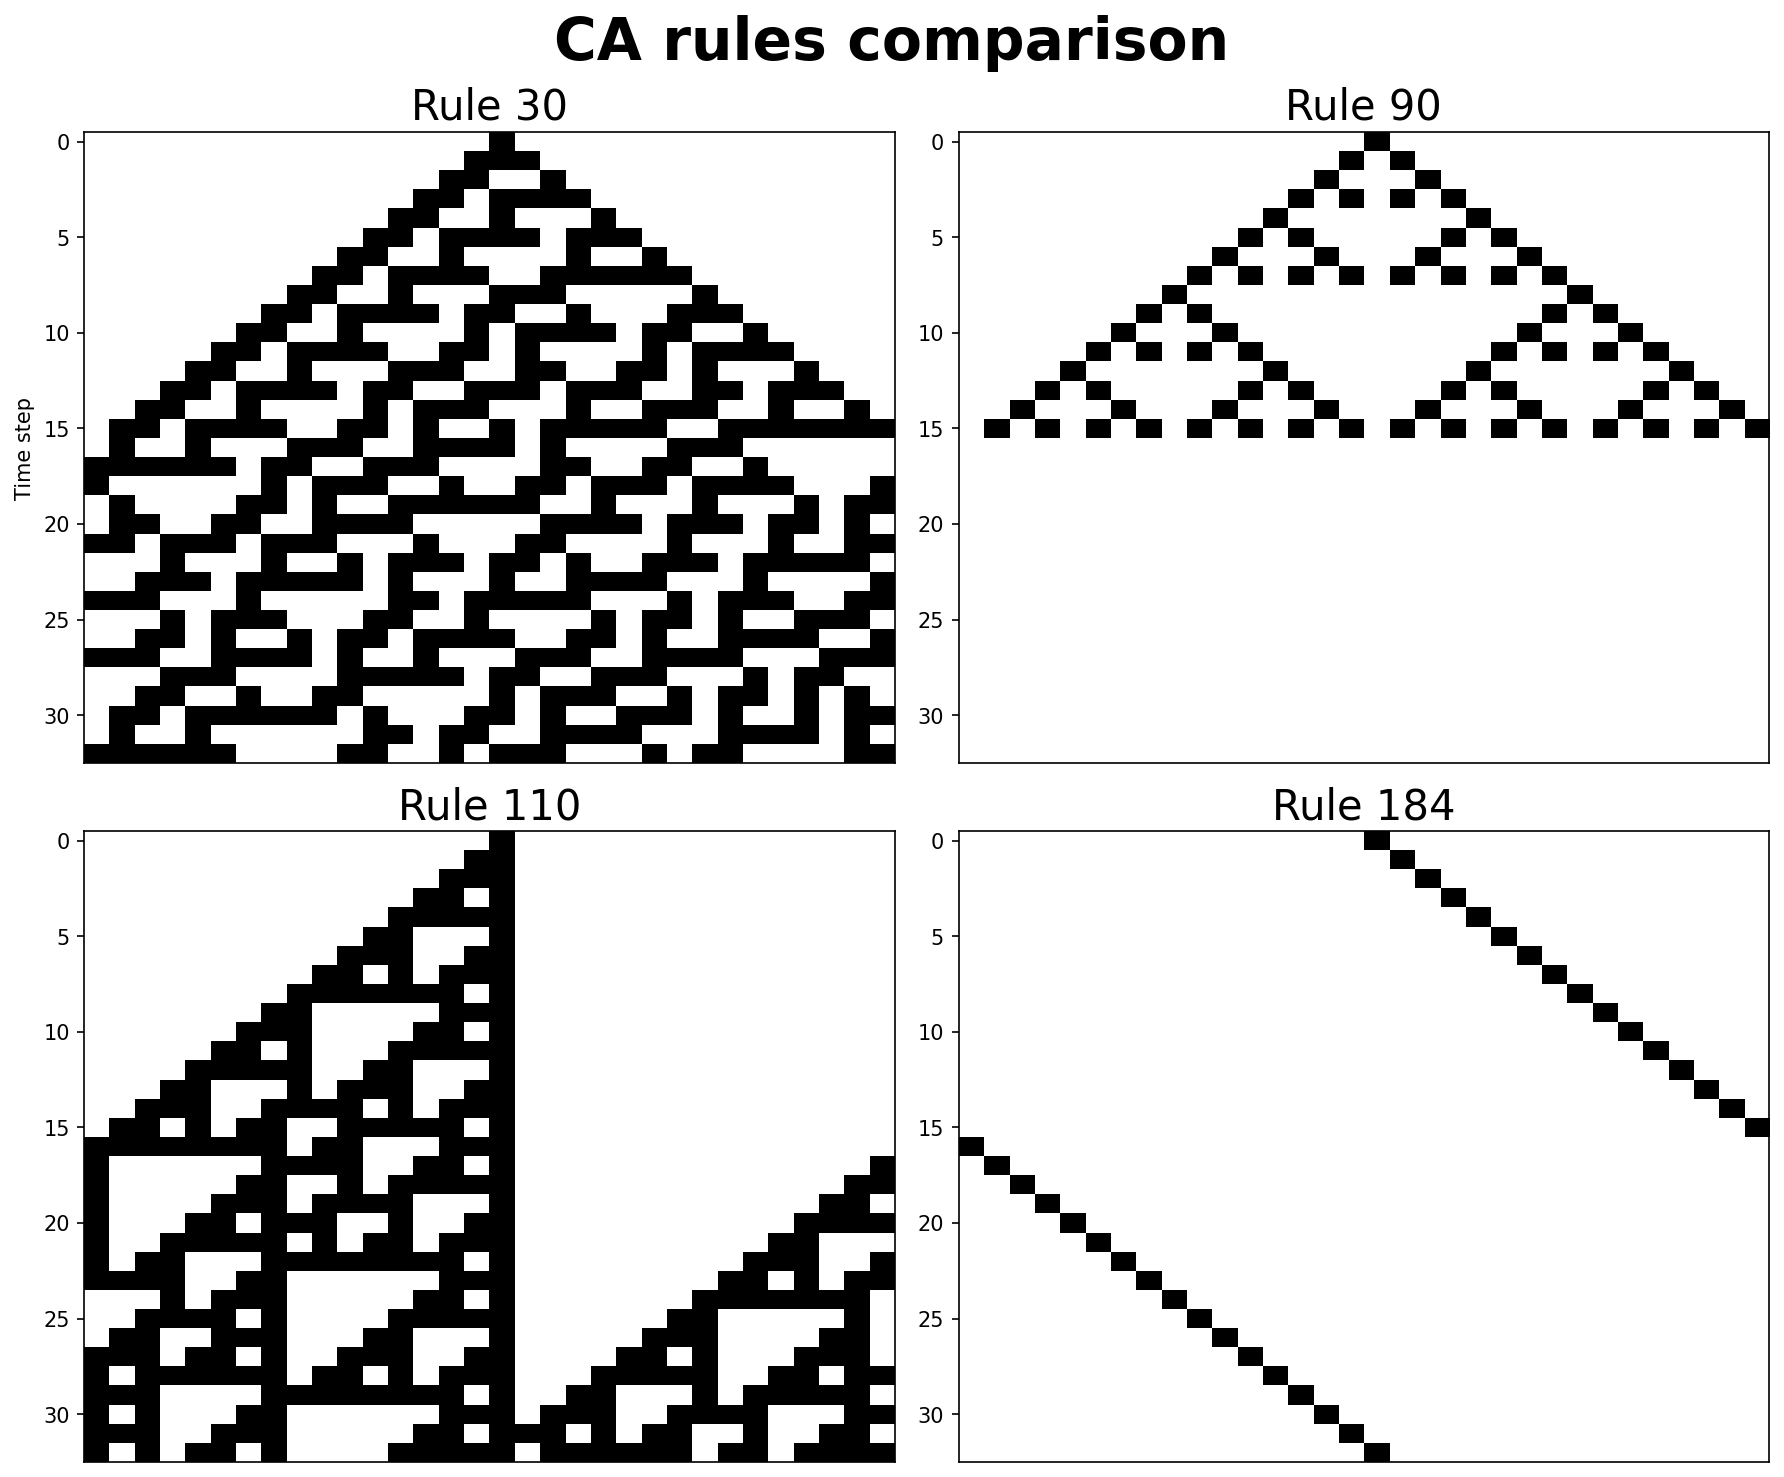
\includegraphics[width=\linewidth]{../results/ca_rules_comparison.png}
    \caption{Comparison of ECA rules trajectories from a simple initial configuration (a single active cell in the center): (top-left) Rule 30, (top-right) Rule 90, (bottom-left) Rule 110, and (bottom-right) Rule 184.}
    \label{fig:trajectory-simple}
\end{figure}

\begin{figure}[ht]
    \centering
    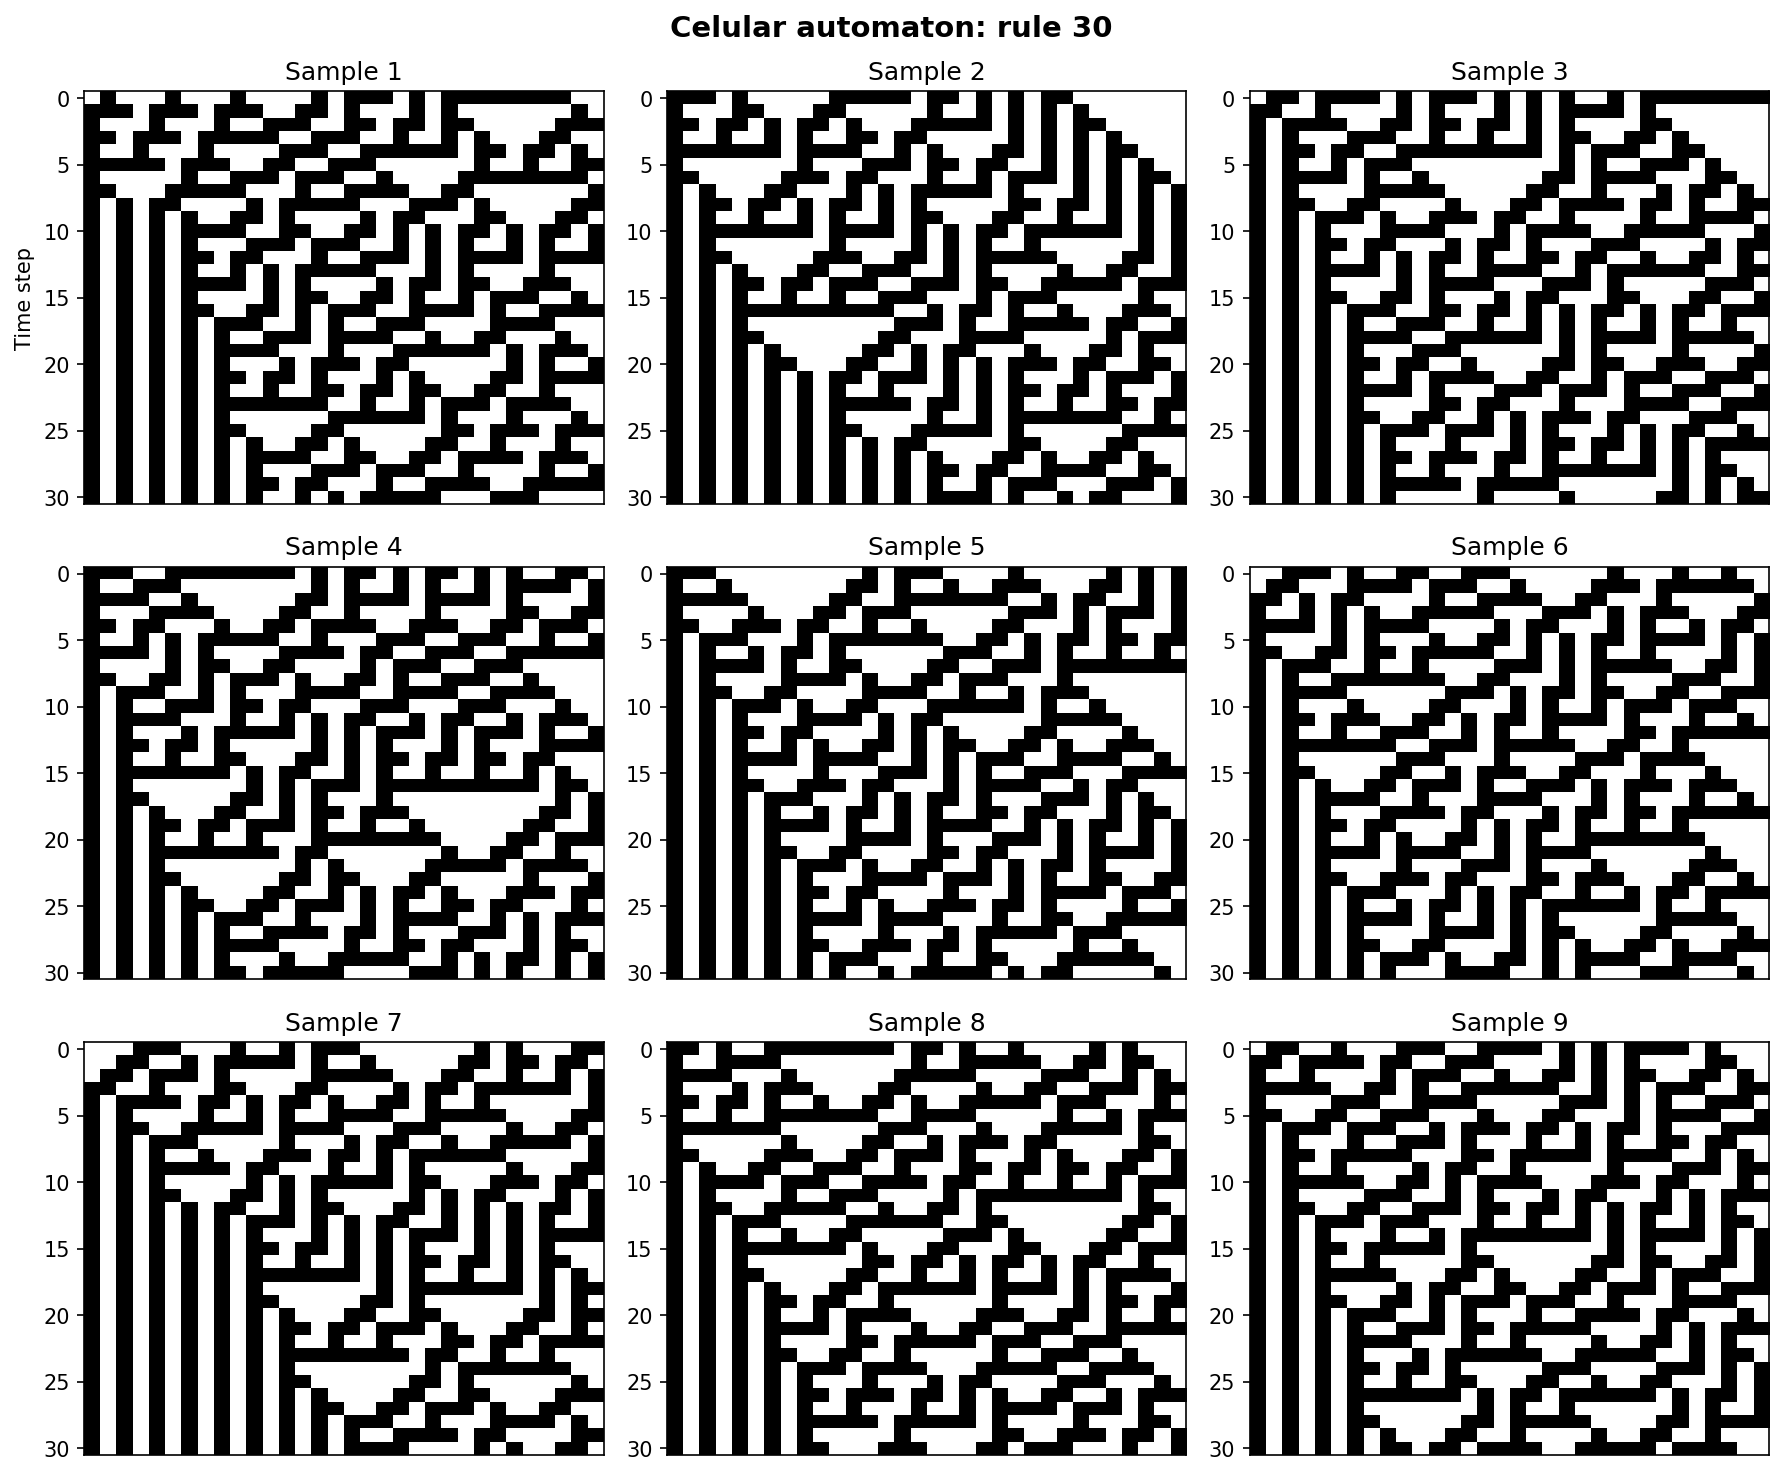
\includegraphics[width=0.45\linewidth]{../results/first_experiment/ca_rule_30.png}
    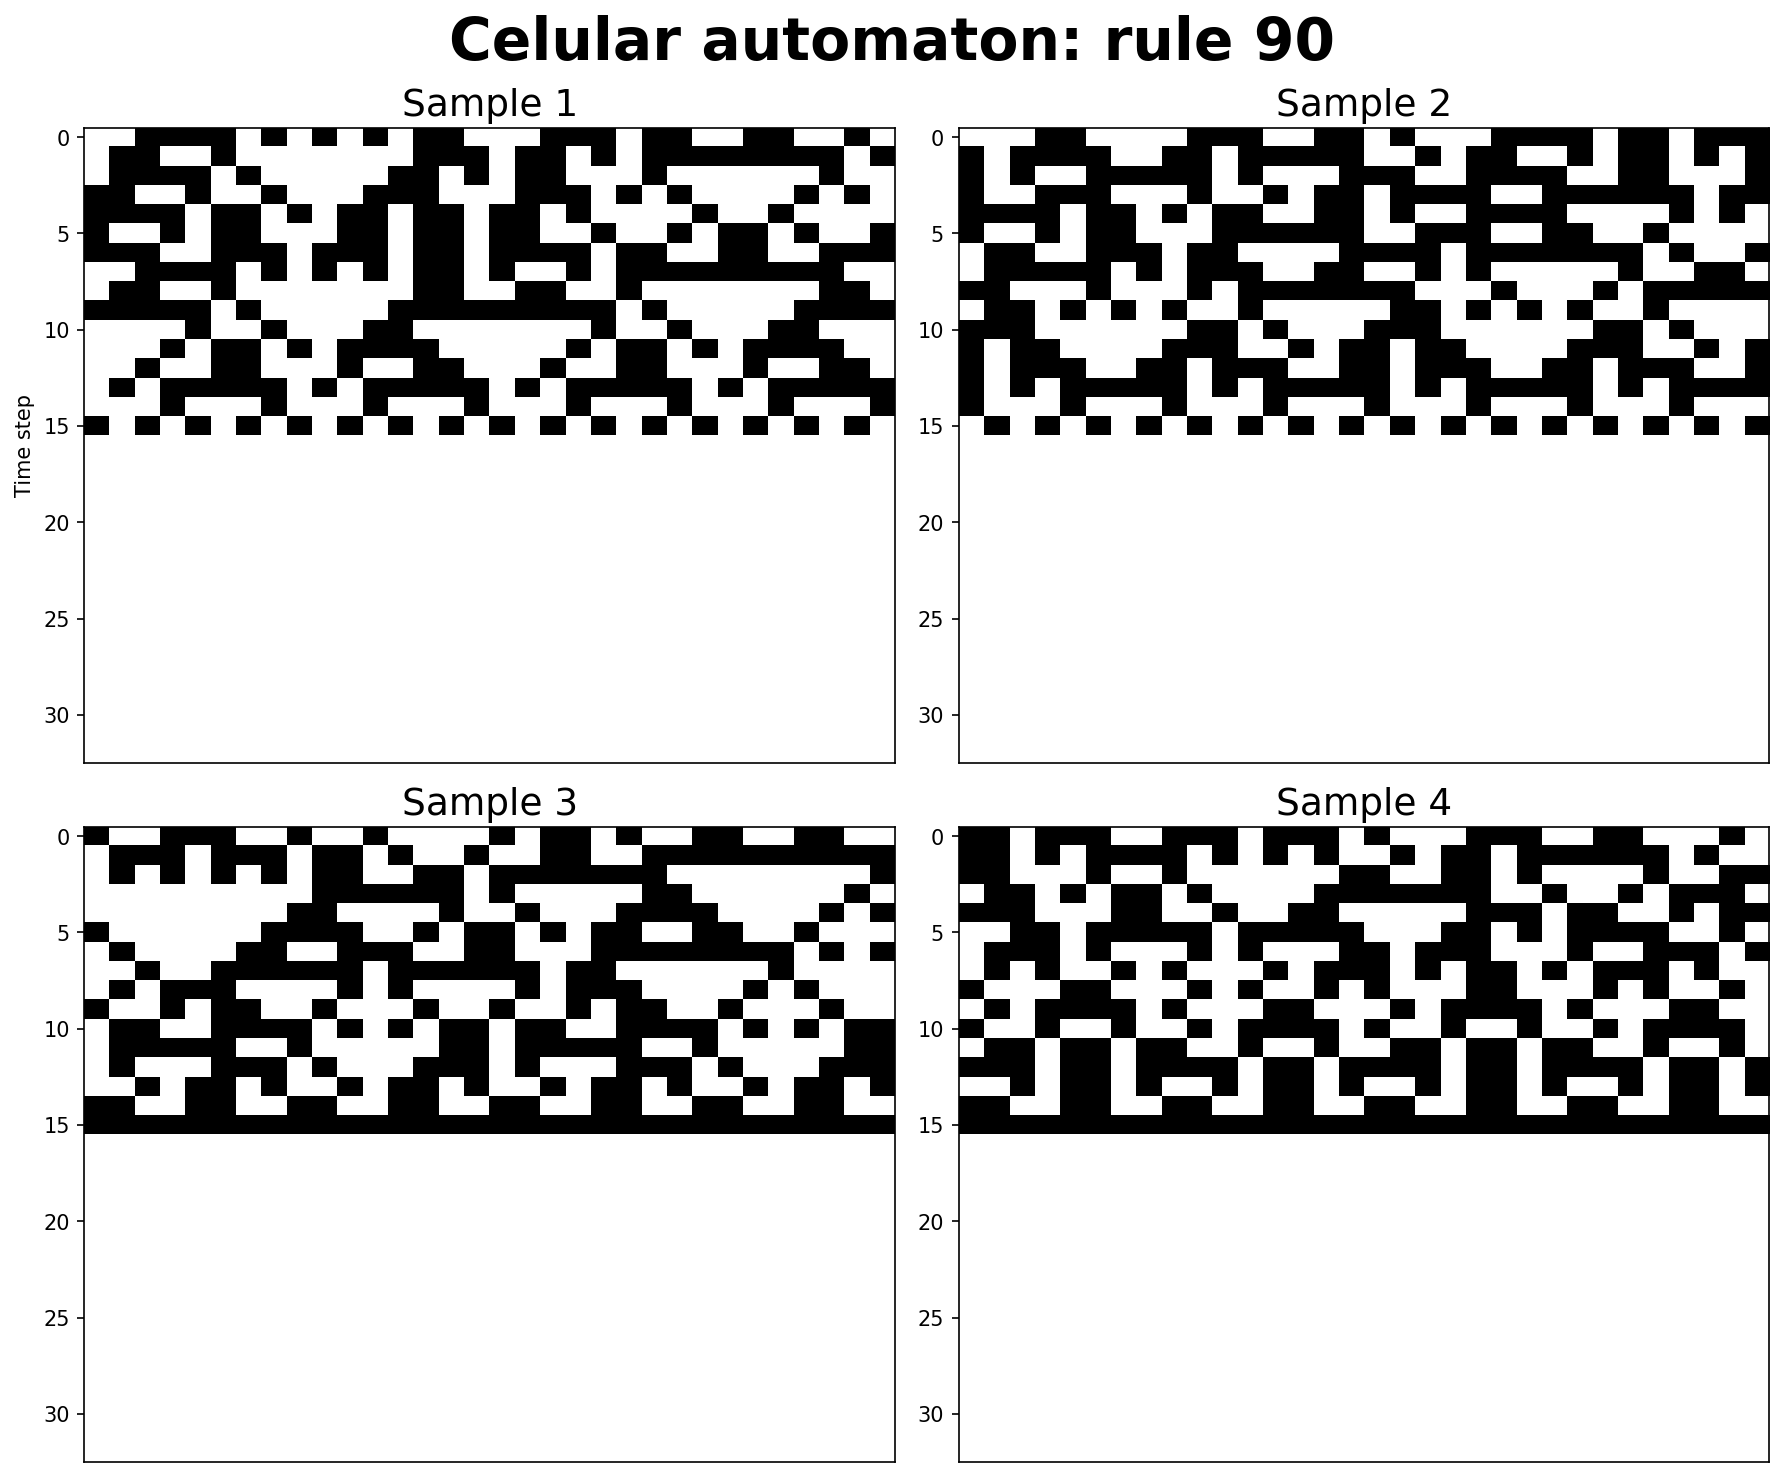
\includegraphics[width=0.45\linewidth]{../results/first_experiment/ca_rule_90.png} \\
    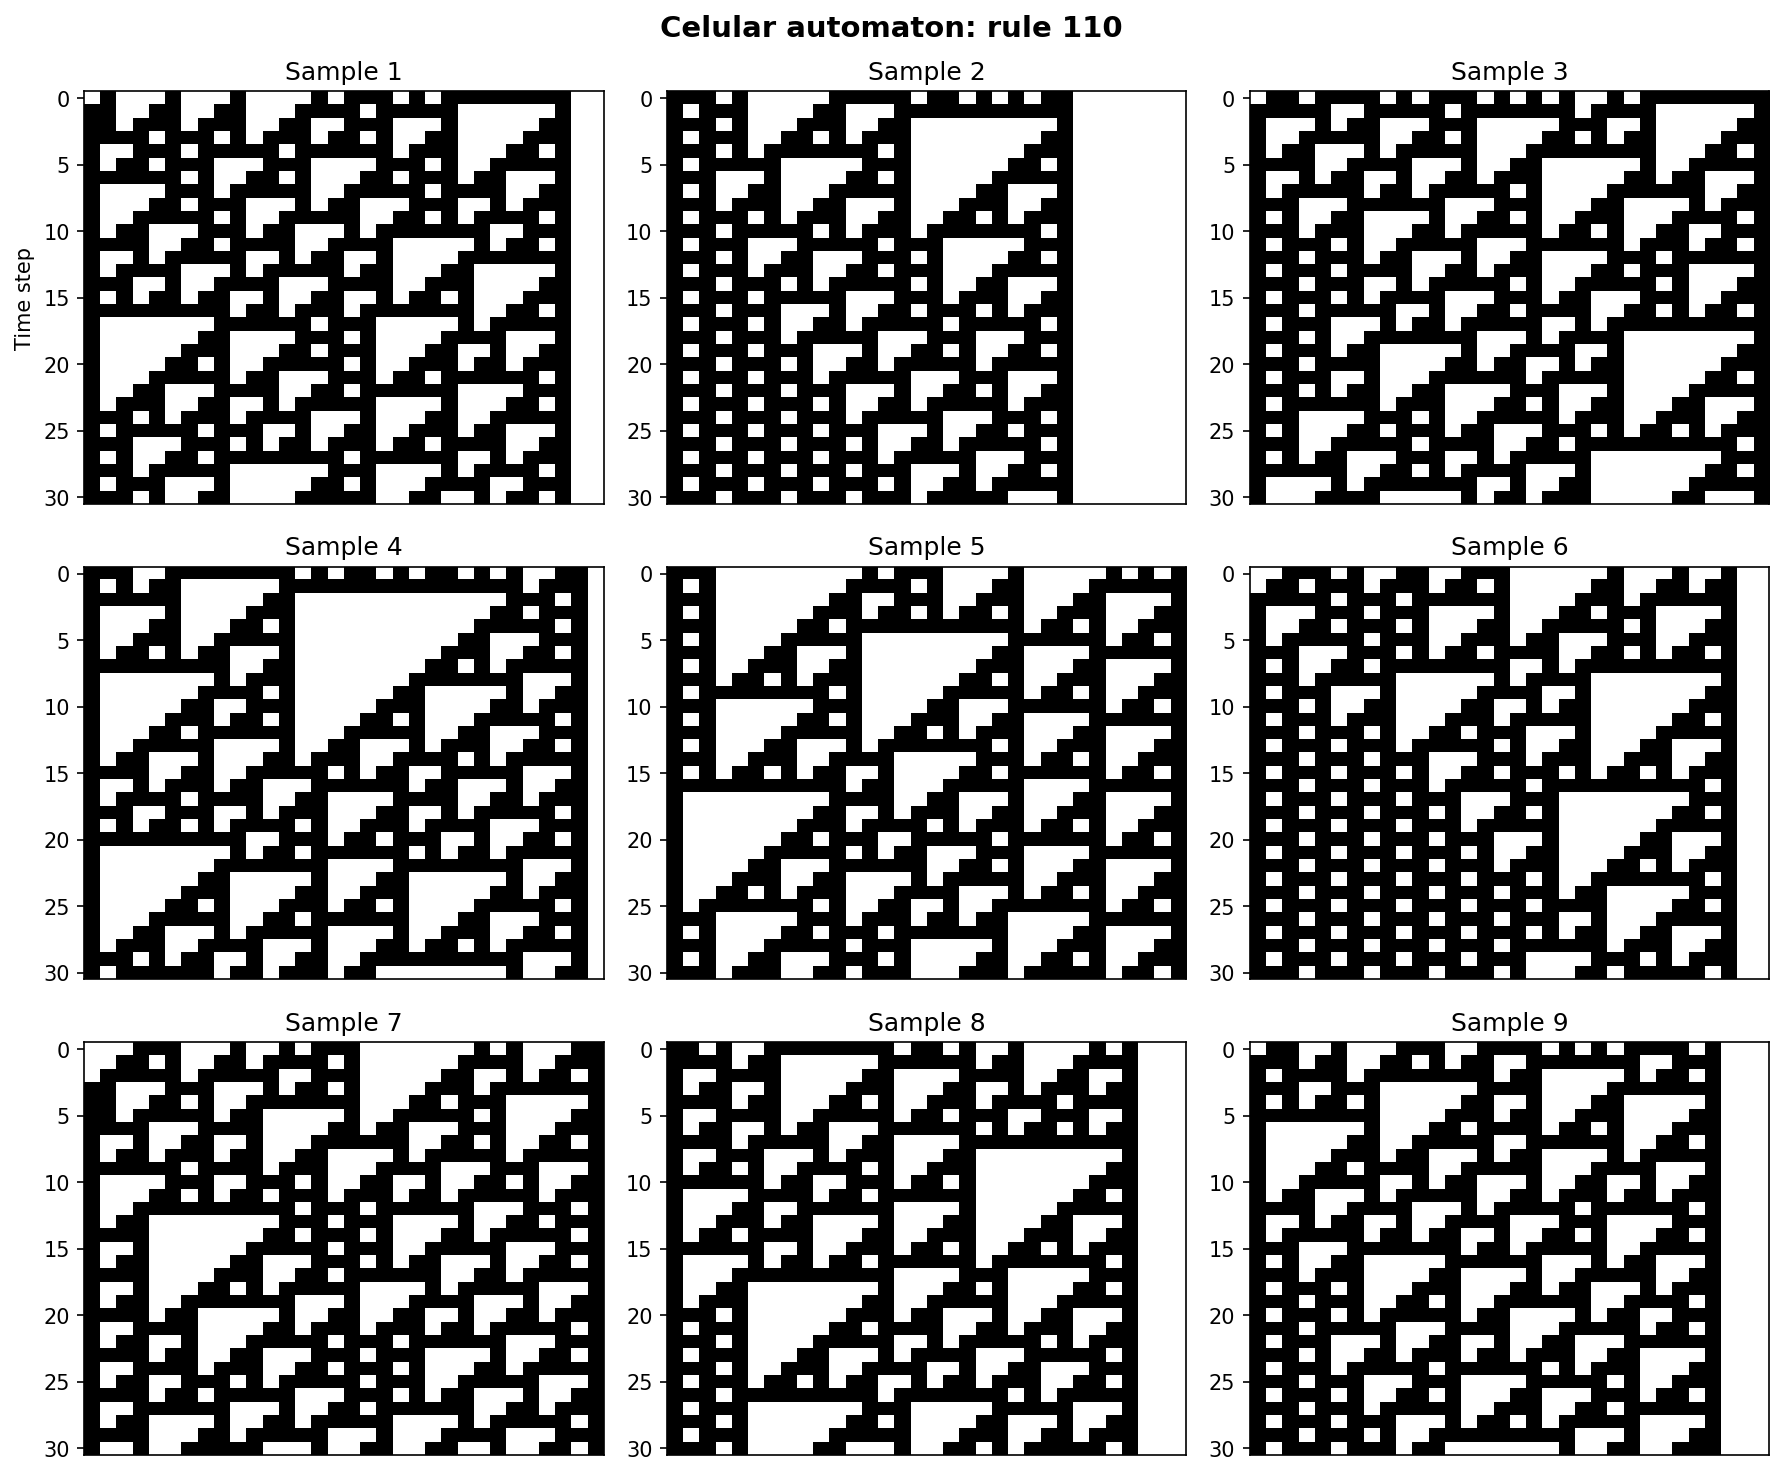
\includegraphics[width=0.45\linewidth]{../results/first_experiment/ca_rule_110.png}
    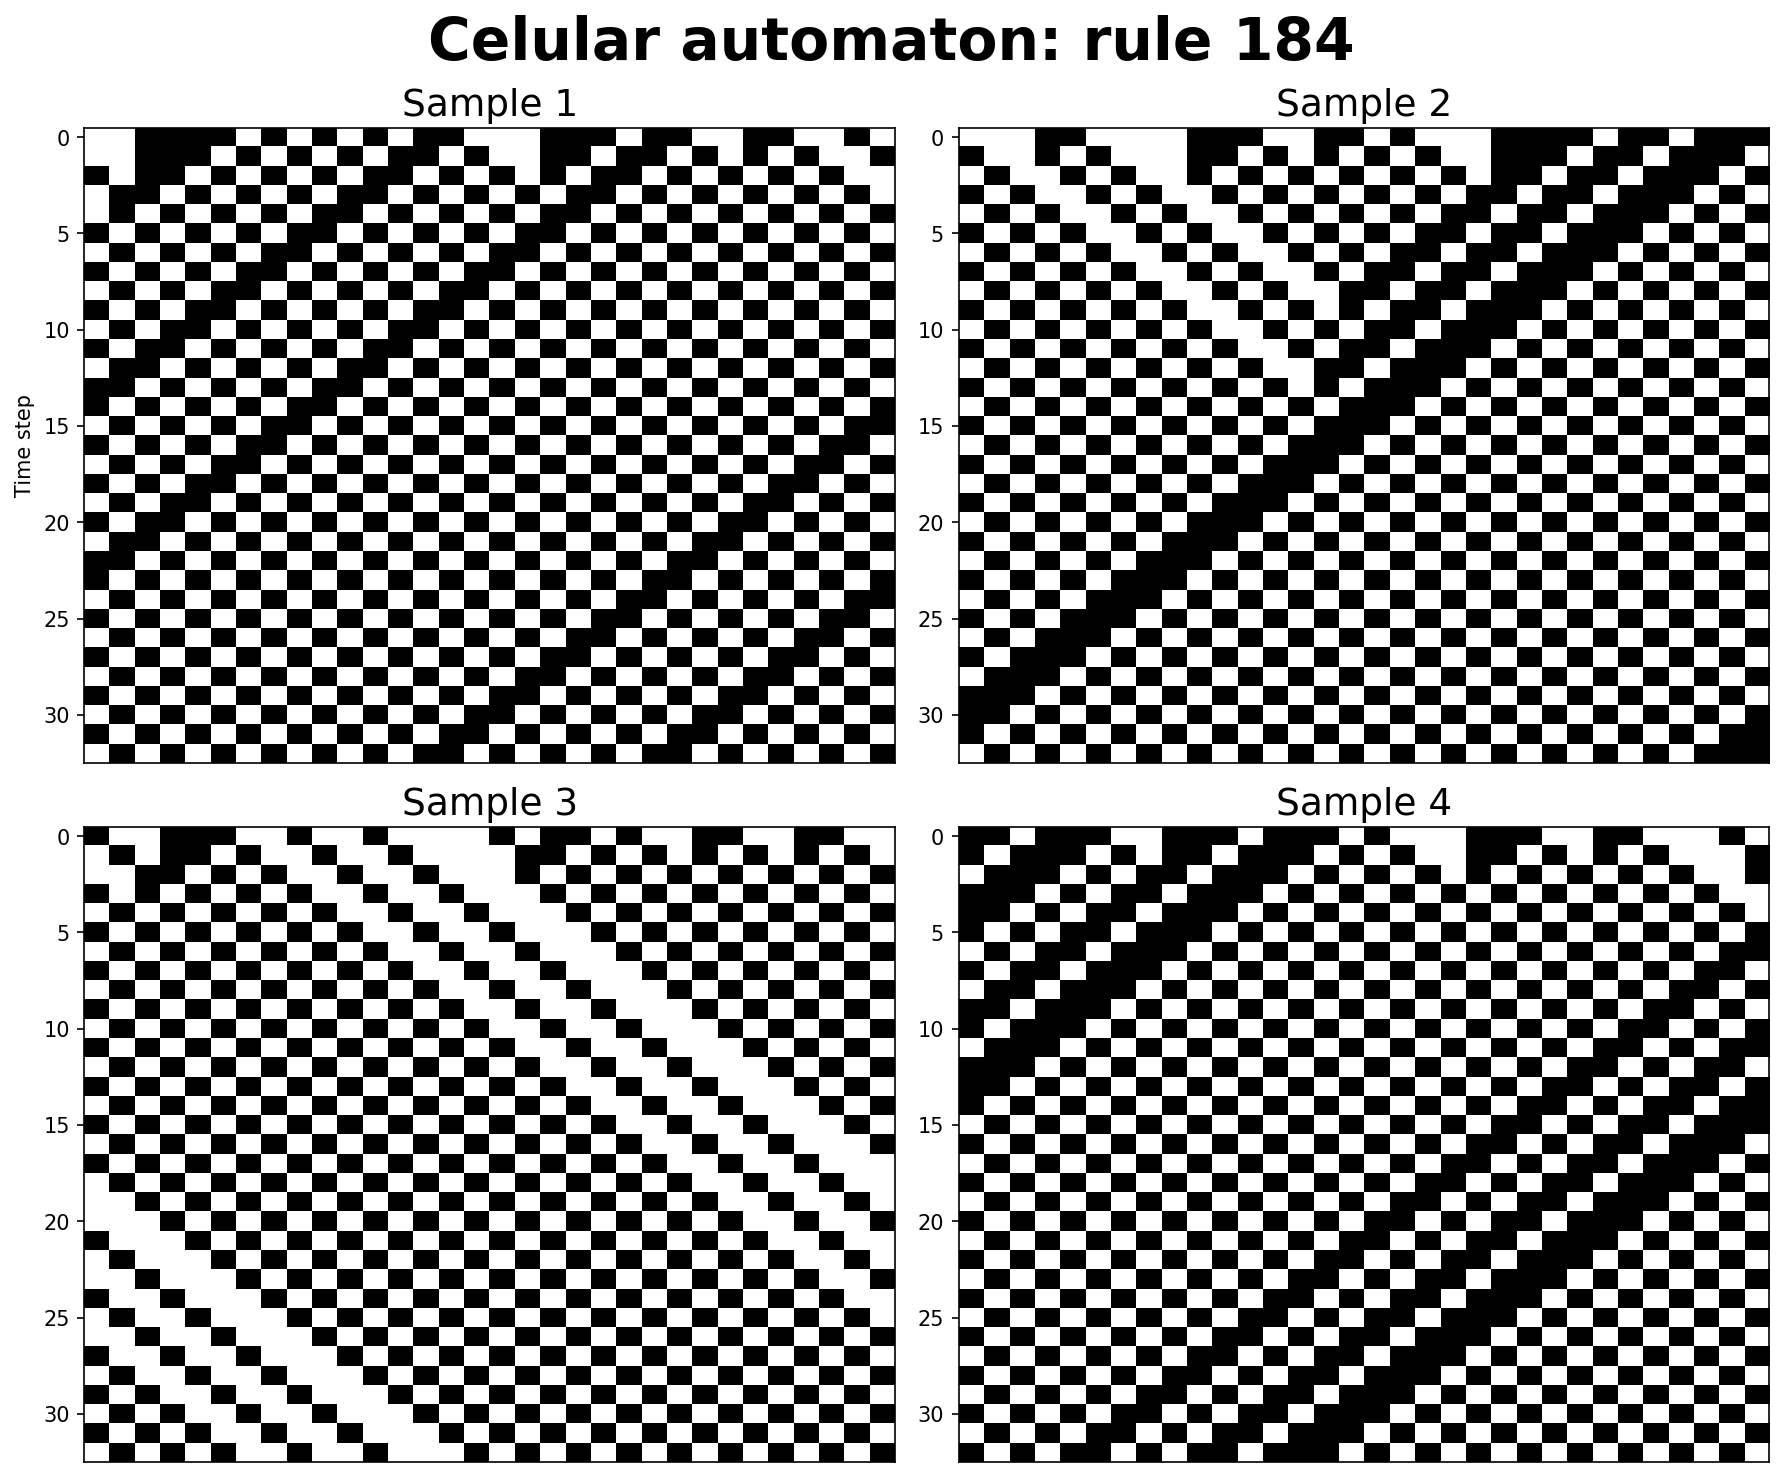
\includegraphics[width=0.45\linewidth]{../results/first_experiment/ca_rule_184.png}
    \caption{Comparison of ECA rules trajectories from random initial states: (top-left) Rule 30, (top-right) Rule 90, (bottom-left) Rule 110, (bottom-right) Rule 184.}
    \label{fig:trajectory-random}
\end{figure}


\subsection{Problem Statement}
\label{sec:problem-statement}

Given a fixed ECA rule $f$ and a dataset of input-output pairs $\{(\mathbf{x}^{(t)}, \mathbf{x}^{(t+1)})\}$ generated by applying the rule to random initial states, the task is to train a Transformer model to learn the mapping from $\mathbf{x}^{(t)}$ to $\mathbf{x}^{(t+1)}$. The model's performance will be evaluated based on the cell-wise accuracy and the sequence-wise accuracy on a test set.

We want to mention that cellular automata prediction can be explored in various ways, such as predicting multiple time steps ahead, learning the underlying rule from observed trajectories, or generalizing to different initial conditions. In Burtsev's work~\cite{burtsev}, they analyzed automata with arbitrary rules and focused on learning the general update dynamics rather than focusing on specific automata. They considered four different learning tasks:

\begin{itemize}
    \item \textit{Orbit-State} -- Given a sequence of states (orbit), predict the immediate next state.
    \item \textit{Orbit-Orbit} -- Given a sequence of states, predict the subsequent states up to a certain time step\dots
    \item \textit{Orbit-State and Rule} -- Given a sequence of states, predict the next state and the underlying local rule.
    \item \textit{Rule and Orbit-State} -- Given the local rule and a sequence of states, predict the next state.
\end{itemize}

This is an interesting research on the general capabilities of Transformers to learn and generalize algorithmic patterns. However, in this project, we focus on the ``State-State'' task for a fixed ECA rule, which is a much simpler problem. We aim to look at the details of the learning dynamics and compare them across rules with different degrees of complexity.


\section{Model Architecture}
\label{sec:model-architecture}

We propose a simple Transformer model consisting of the following components:

\begin{enumerate}
    \item \textbf{Token Embedding Layer:} An embedding layer that maps binary values (0 or 1) to a dense vector of dimension $d_{\text{model}}$.
    
    \item \textbf{Positional Embedding:} A learnable positional encoding added to the token embeddings.
    
    \item \textbf{Transformer Encoder:} A stack of Transformer encoder layers, each consisting of multi-head self-attention and feed-forward sub-layers with residual connections and layer normalization.
    
    \item \textbf{Output Projection:} A linear layer that projects the encoded representations back to the binary space, producing logits for each cell's next state.
\end{enumerate}


\subsection{Hyperparameters}
\label{sec:hyperparameters}

The Transformer model uses the following hyperparameters:

\begin{itemize}
    \item model dimension: $d_{\text{model}} = 64$
    \item number of attention heads: $n_{\text{heads}} = 4$
    \item number of encoder layers: $n_{\text{layers}} = 2$
    \item feedforward dimension: $d_{\text{ff}} = 128$
    \item dropout probability: $p_{\text{dropout}} = 0.1$
    \item activation function: GELU
\end{itemize}

The model is trained using the Adam optimizer with learning rate $\text{lr} = 10^{-3}$ and cross-entropy loss.


\subsection{Comparison to Previous Work}
\label{sec:comparison}

Compared to the work by Burtsev~\cite{burtsev}, our model is significantly smaller. Burtsev used the same Transformer model with full self-attention, but with $d_{\text{model}} = 512$, $n_{\text{heads}} = 8$, and $n_{\text{layers}} = 4$.

However, they worked with cellular automata of width $W = 20$ and radius $r = 2$. In contrast, we focus on ECA with $W = 32$ and $r = 1$ (see \cref{sec:experimental-setup}), which has a smaller input space and simpler dynamics.

They also use a slightly larger input vocabulary, including special token [SEP] for separating multiple states in the input and mask token [M], which takes place of the state or rule to be predicted.


\section{First Experiment}
\label{sec:first-experiment}

In the first experiment, we evaluate the Transformer model's ability to predict the next state given the current state with fixed sequence length for four different ECA rules: Rule 30, Rule 90, Rule 110, and Rule 184. These rules exhibit diverse patterns, ranging from ordered (rules 90 and 184) to chaotic dynamics (rules 30 and 110).

We initially expected that Rules 90 and 184 will be easier for the Transformer to learn than Rules 30 and 110, since their update dynamics are more regular and structured, whereas Rules 30 and 110 exhibit more complex or chaotic behavior. However, we got quite the opposite results, more details in \cref{sec:results}.


\subsection{Experimental Setup}
\label{sec:experimental-setup}

We work with a fixed width of $W = 32$ cells. For each rule, we generate a dataset of input-output pairs by sampling random binary initial states and applying the rule for one time step.

The dataset sizes are:
\begin{itemize}
    \item Training set: $100{,}000$ samples per rule
    \item Test set: $10{,}000$ samples per rule
\end{itemize}

We use a batch size of $128$ for training and the model is trained for $20$ epochs. We measured the training loss and also evaluated accuracy metrics after each epoch.


\subsection{Results}
\label{sec:results}

The model's training progress for each rule is shown in \cref{fig:loss-history} and accuracy metrics progress is shown in \cref{fig:eval-history}. All four rules were successfully learned by the model, achieving near-zero training loss and perfect, 100\% accuracy on the test set.

\begin{figure}[ht]
    \centering
    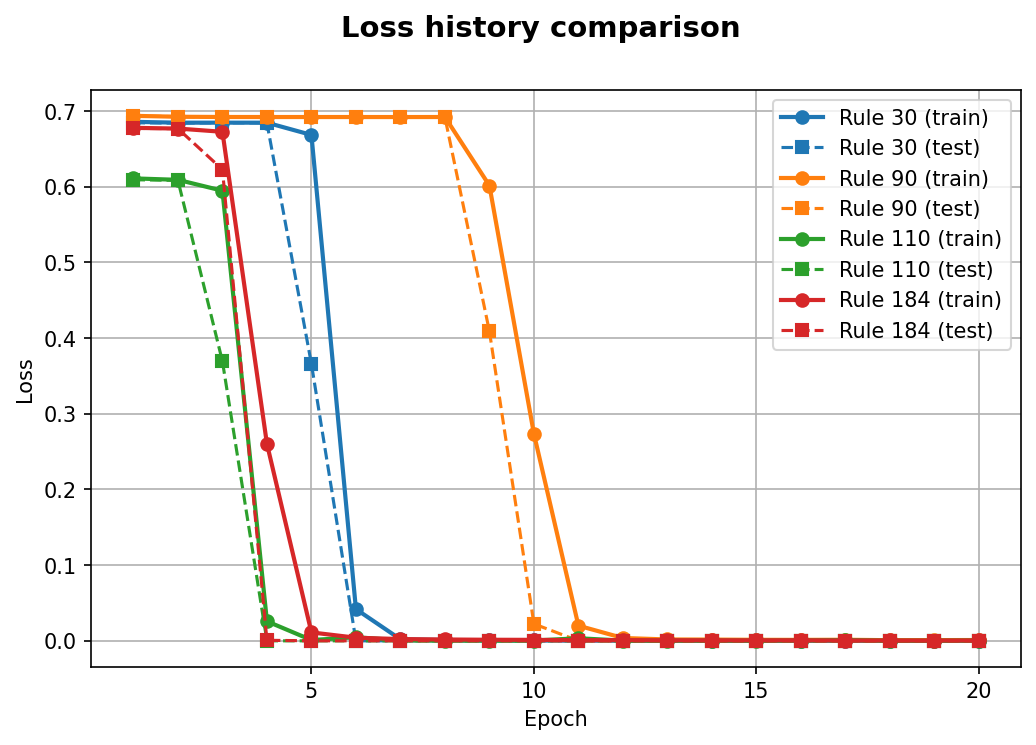
\includegraphics[width=\linewidth]{../results/first_experiment/loss_history_comparison.png}
    \caption{Training loss comparison across all four cellular automaton rules. Loss is computed as per-cell cross-entropy.}
    \label{fig:loss-history}
\end{figure}

\begin{figure}[ht]
    \centering
    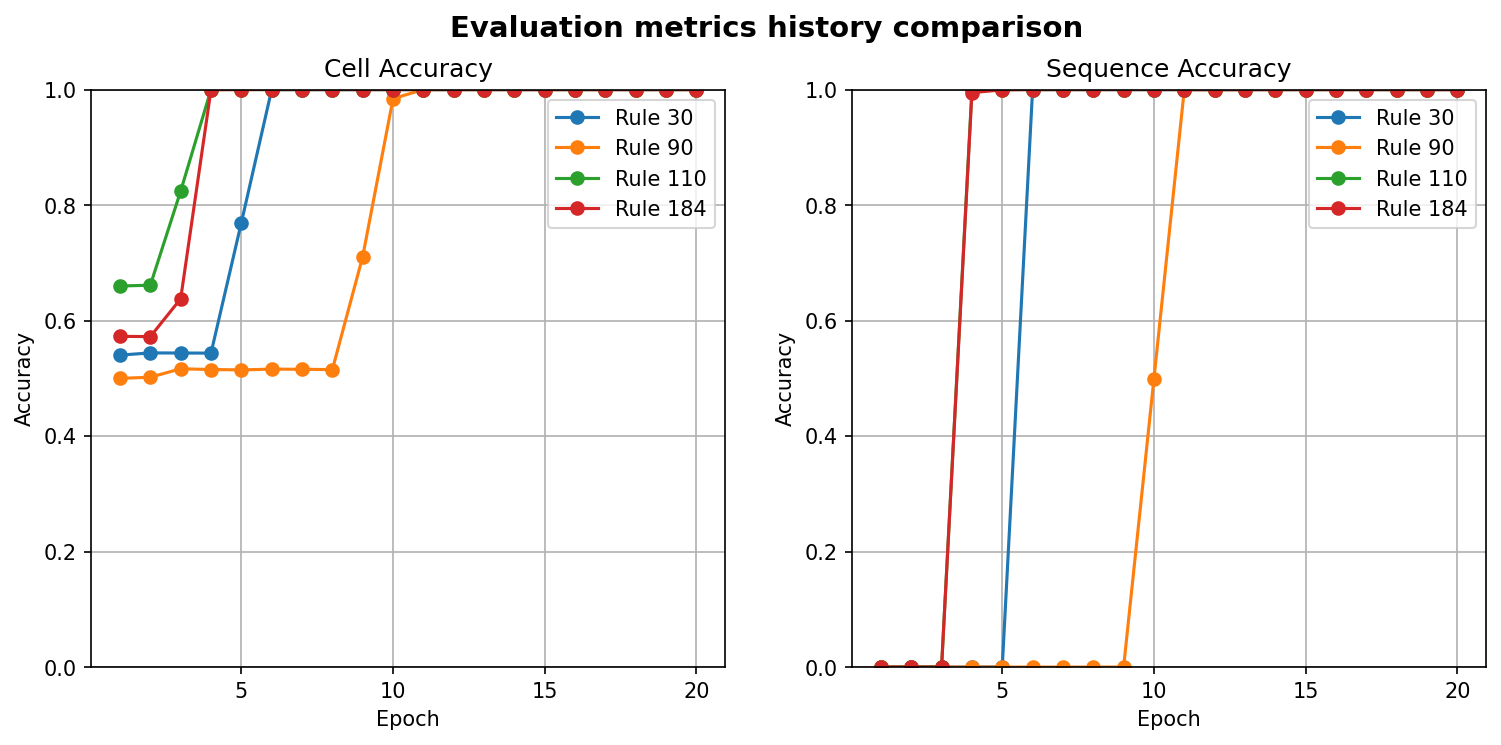
\includegraphics[width=\linewidth]{../results/first_experiment/eval_history_comparison.png}
    \caption{Evaluation metrics comparison during training: (left) cell-wise accuracy, (right) sequence-wise accuracy.}
    \label{fig:eval-history}
\end{figure}

Training loss of all rules started at around $\ln(2) \approx 0.693$ (random guessing in a binary classification task), then dropped rapidly to near-zero values. This sudden drop in loss is a common phenomenom when training transformers on algorithmic tasks, called ``abrupt learning''~\cite{abrupt-learning} or ``grokking''~\cite{grokking}. It is often interpreted as the model gradually organizing its internal representations until it suddenly discovers a generalizable solution -- in this case, the underlying local ECA rule.

The duration of the initial plateau varied across rules -- Rules 110 and 184 started converging fastest (epoch 3), followed by Rule 30 (epoch 5), while Rule 90 exhibited a much longer plateau, only starting converging around epoch 9. The evaluation metrics confirm this behavior, reaching perfect accuracy around the same epochs as the loss convergence.

These results don't really support our initial hypothesis that Rules 90 and 184 would be easier to learn than Rules 30 and 110. In fact, Rule 90 was the most difficult to optimize, despite the fact that it's based on a simple XOR operation. On the other hand, Rule 30 and more surprisingly Rule 110, which have much more complex dynamics, were learned much faster than Rule 90.

We also analyzed the attention maps of the trained models for both layers, shown in \cref{fig:attention}. The attention weights were averaged across all test samples. All four rules show a similar diagonal pattern in some of their attention heads, which indicates that the model is attending to the local information. This is expected behavior since ECA rules are local. We can also see some heads with diffuse attention patterns, most notably in Rule 110 first layer. On the other hand, Rule 30 displays the diagonal pattern most clearly out of all rules.

\begin{figure}[ht]
    \centering
    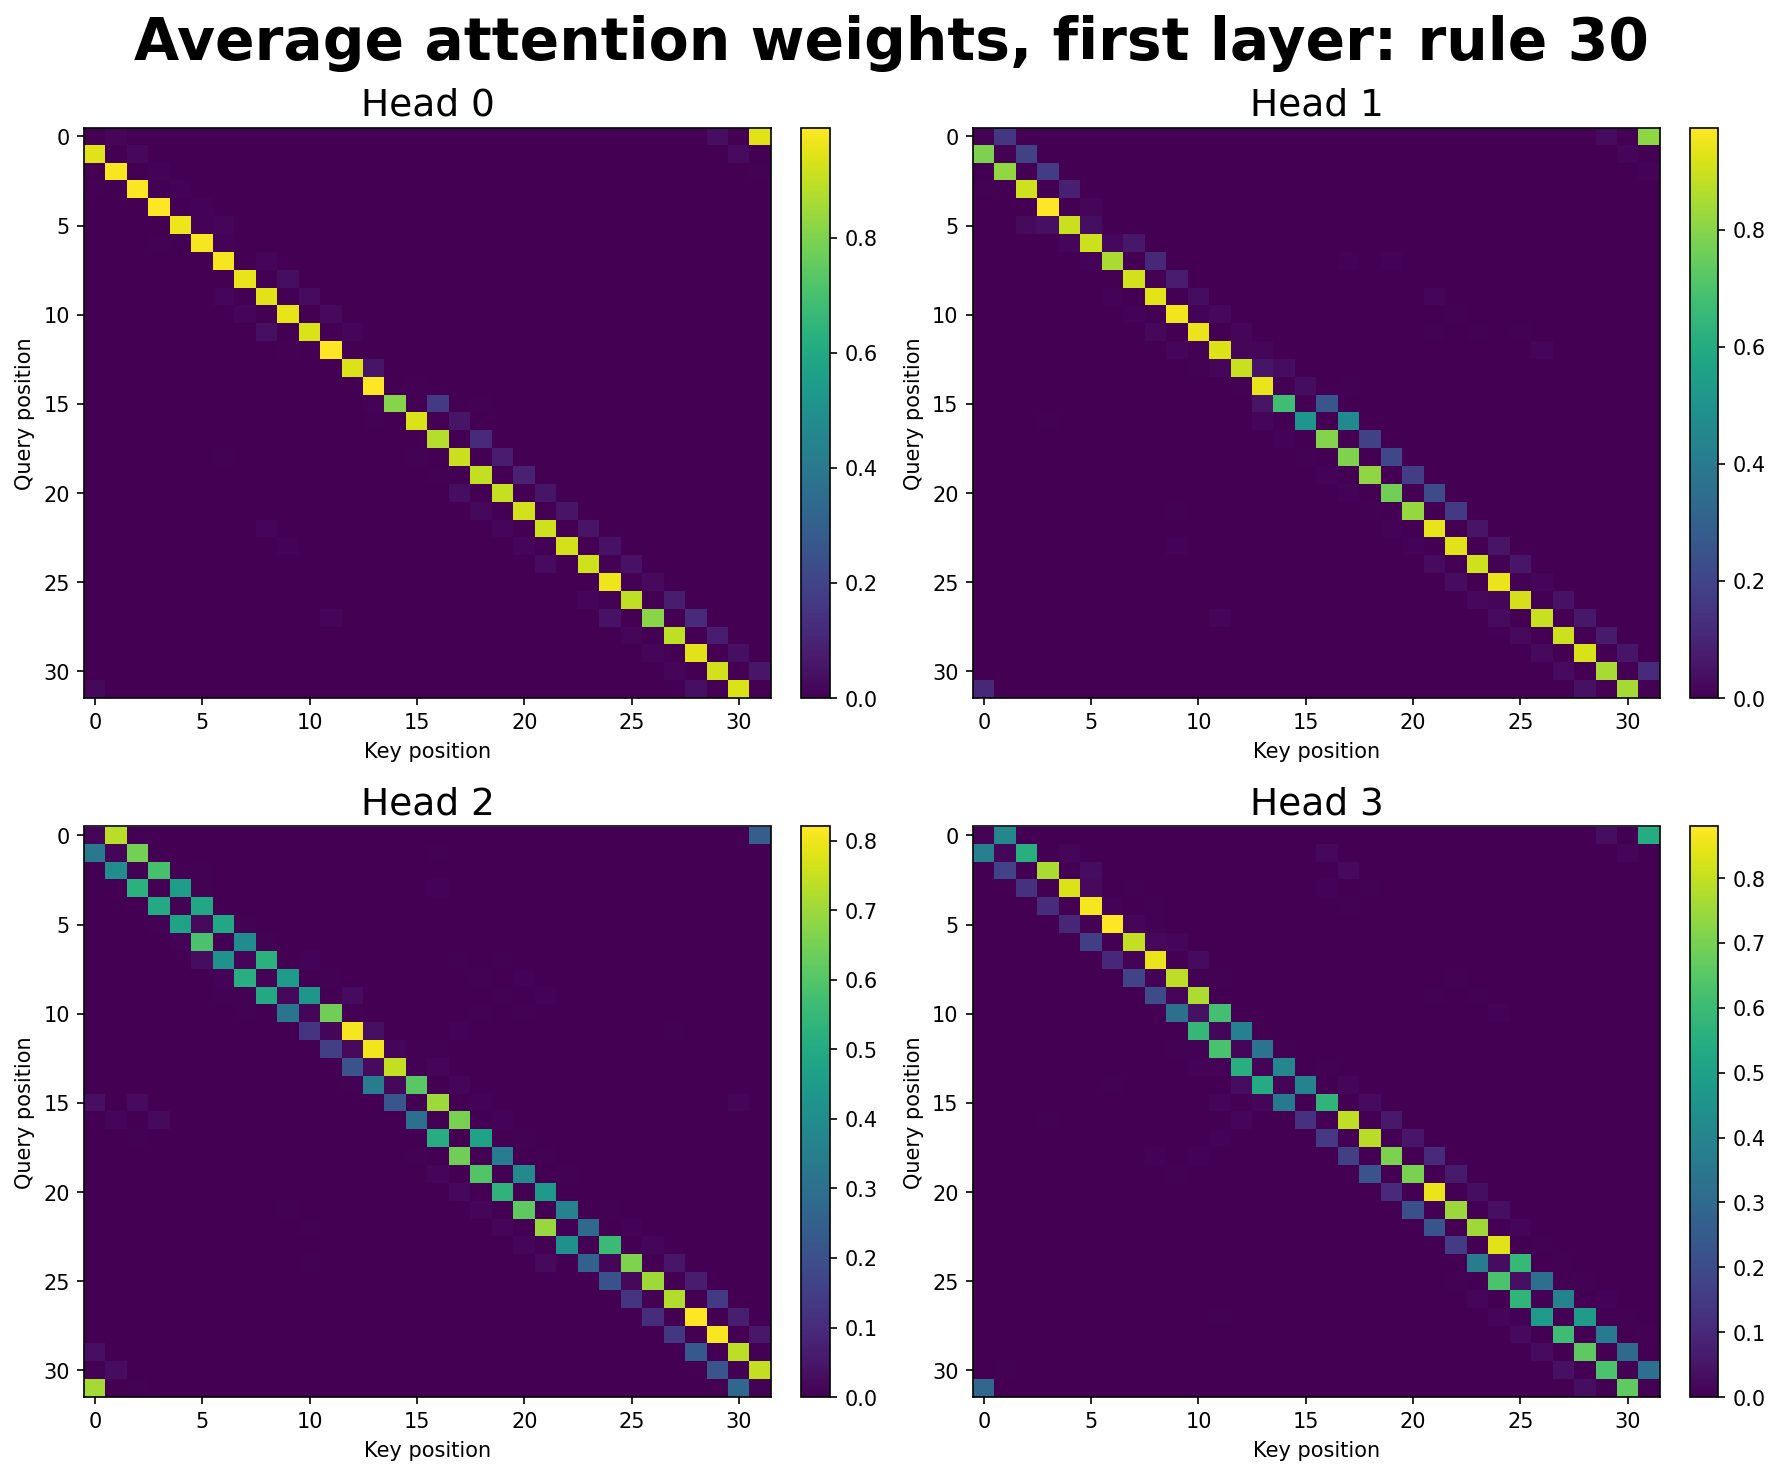
\includegraphics[width=0.45\linewidth]{../results/first_experiment/attention_layer_0_rule_30.png}
    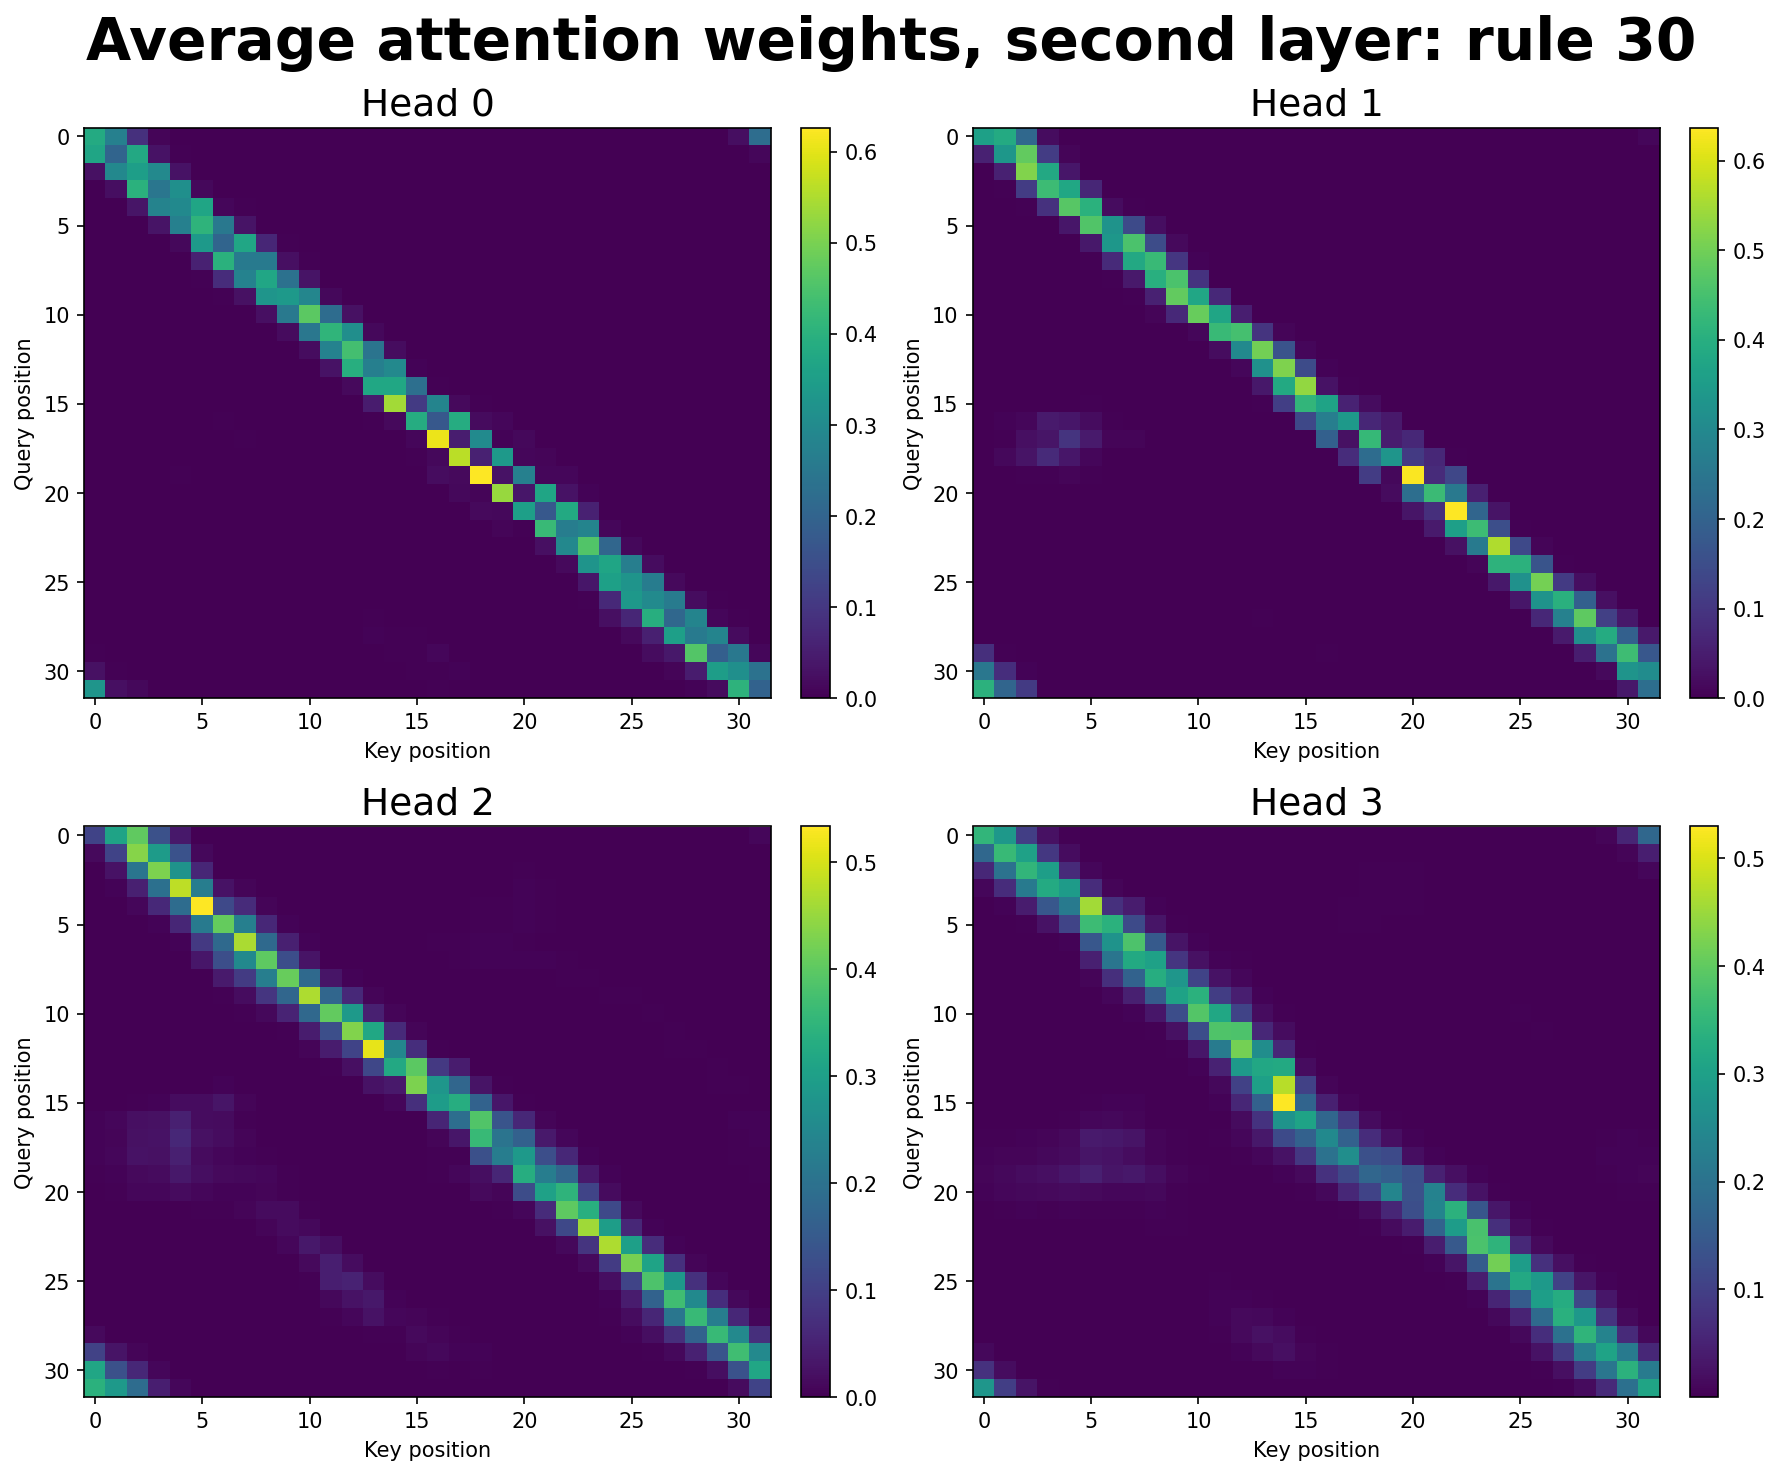
\includegraphics[width=0.45\linewidth]{../results/first_experiment/attention_layer_1_rule_30.png} \\
    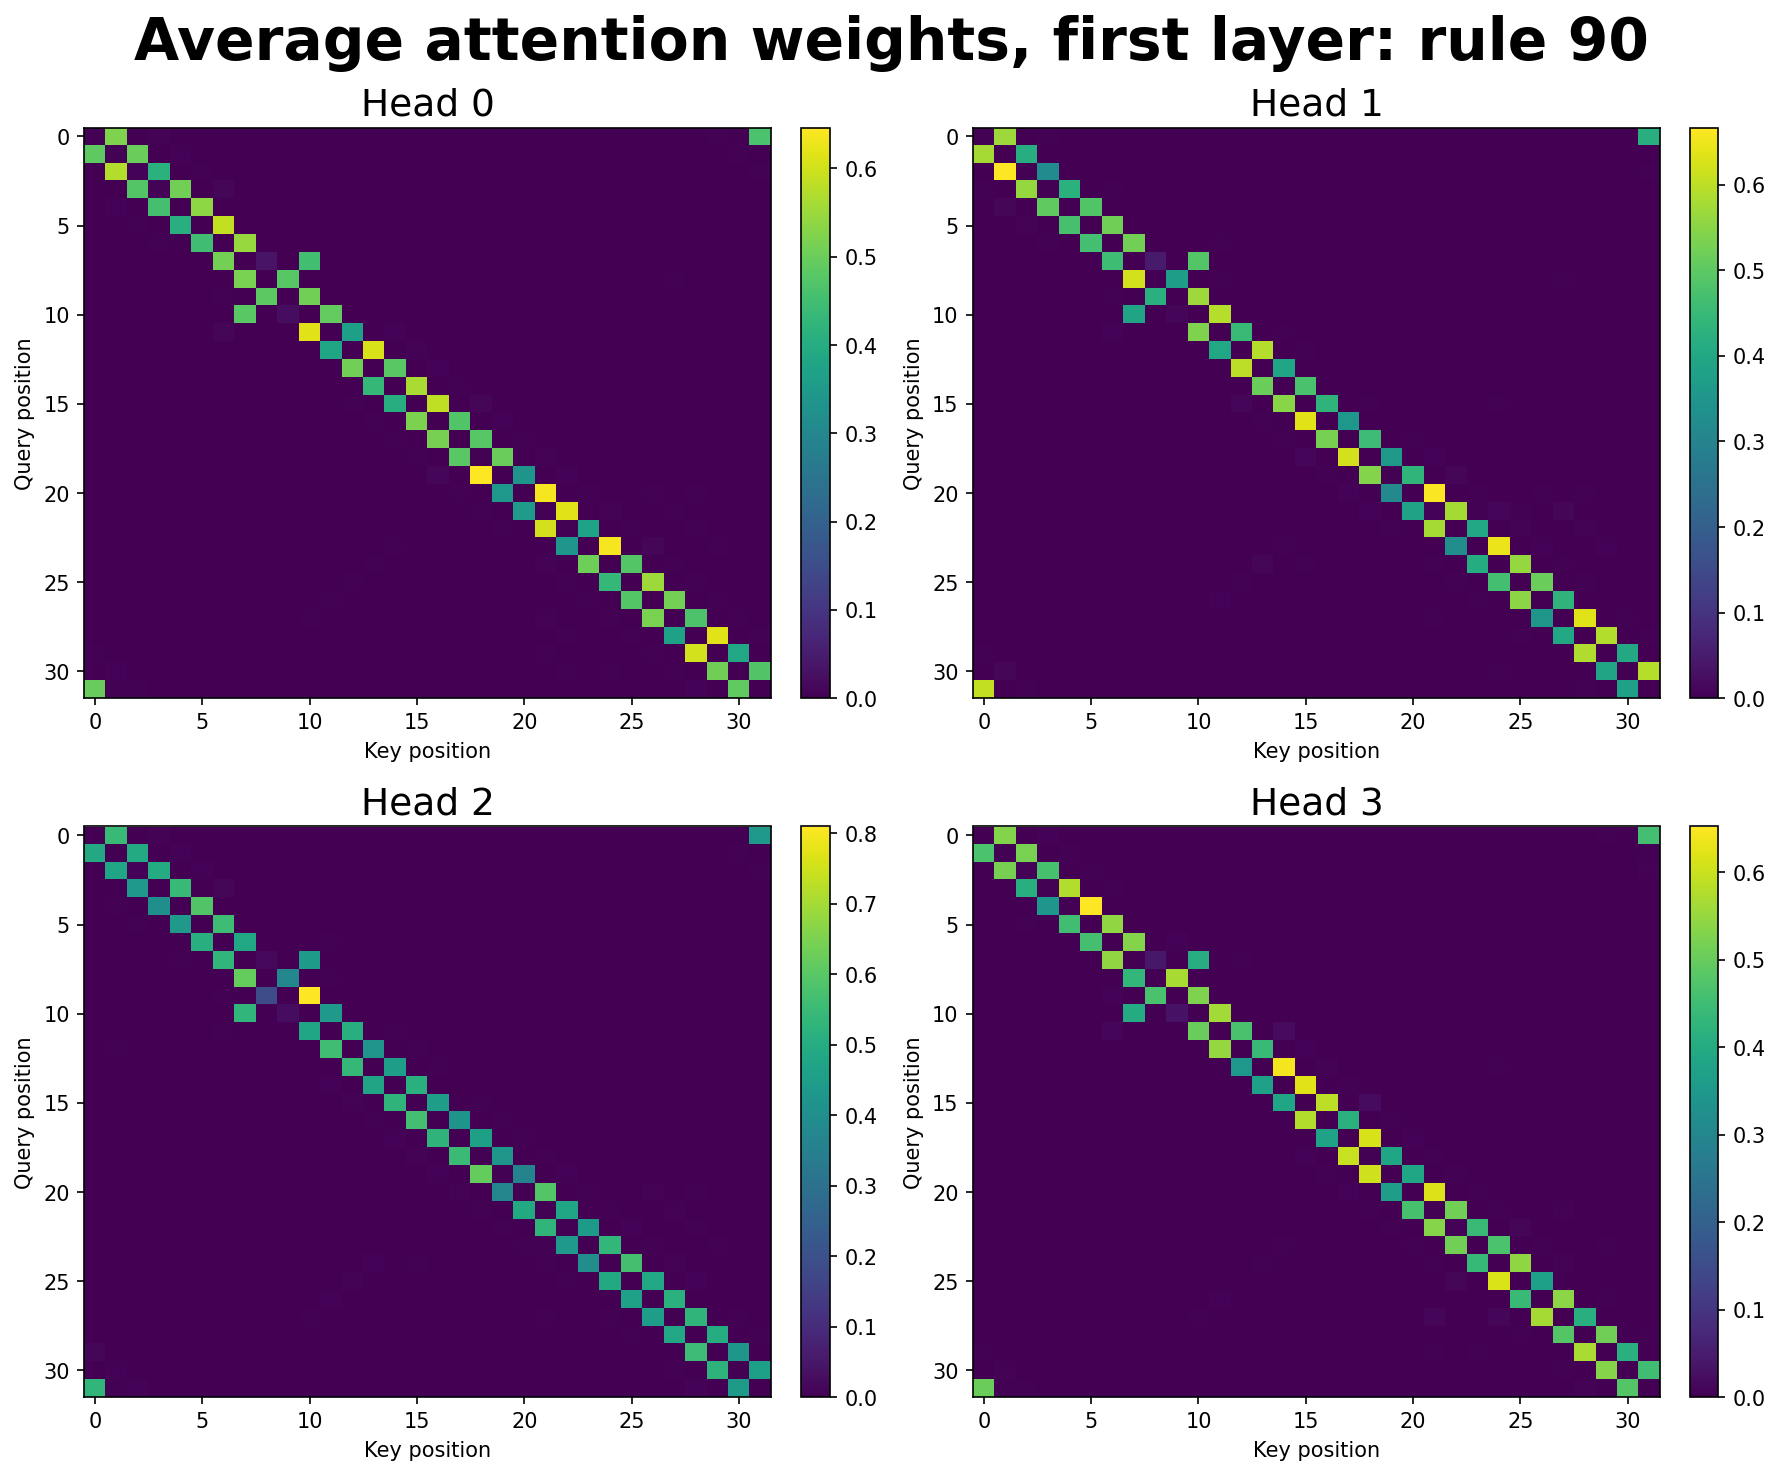
\includegraphics[width=0.45\linewidth]{../results/first_experiment/attention_layer_0_rule_90.png}
    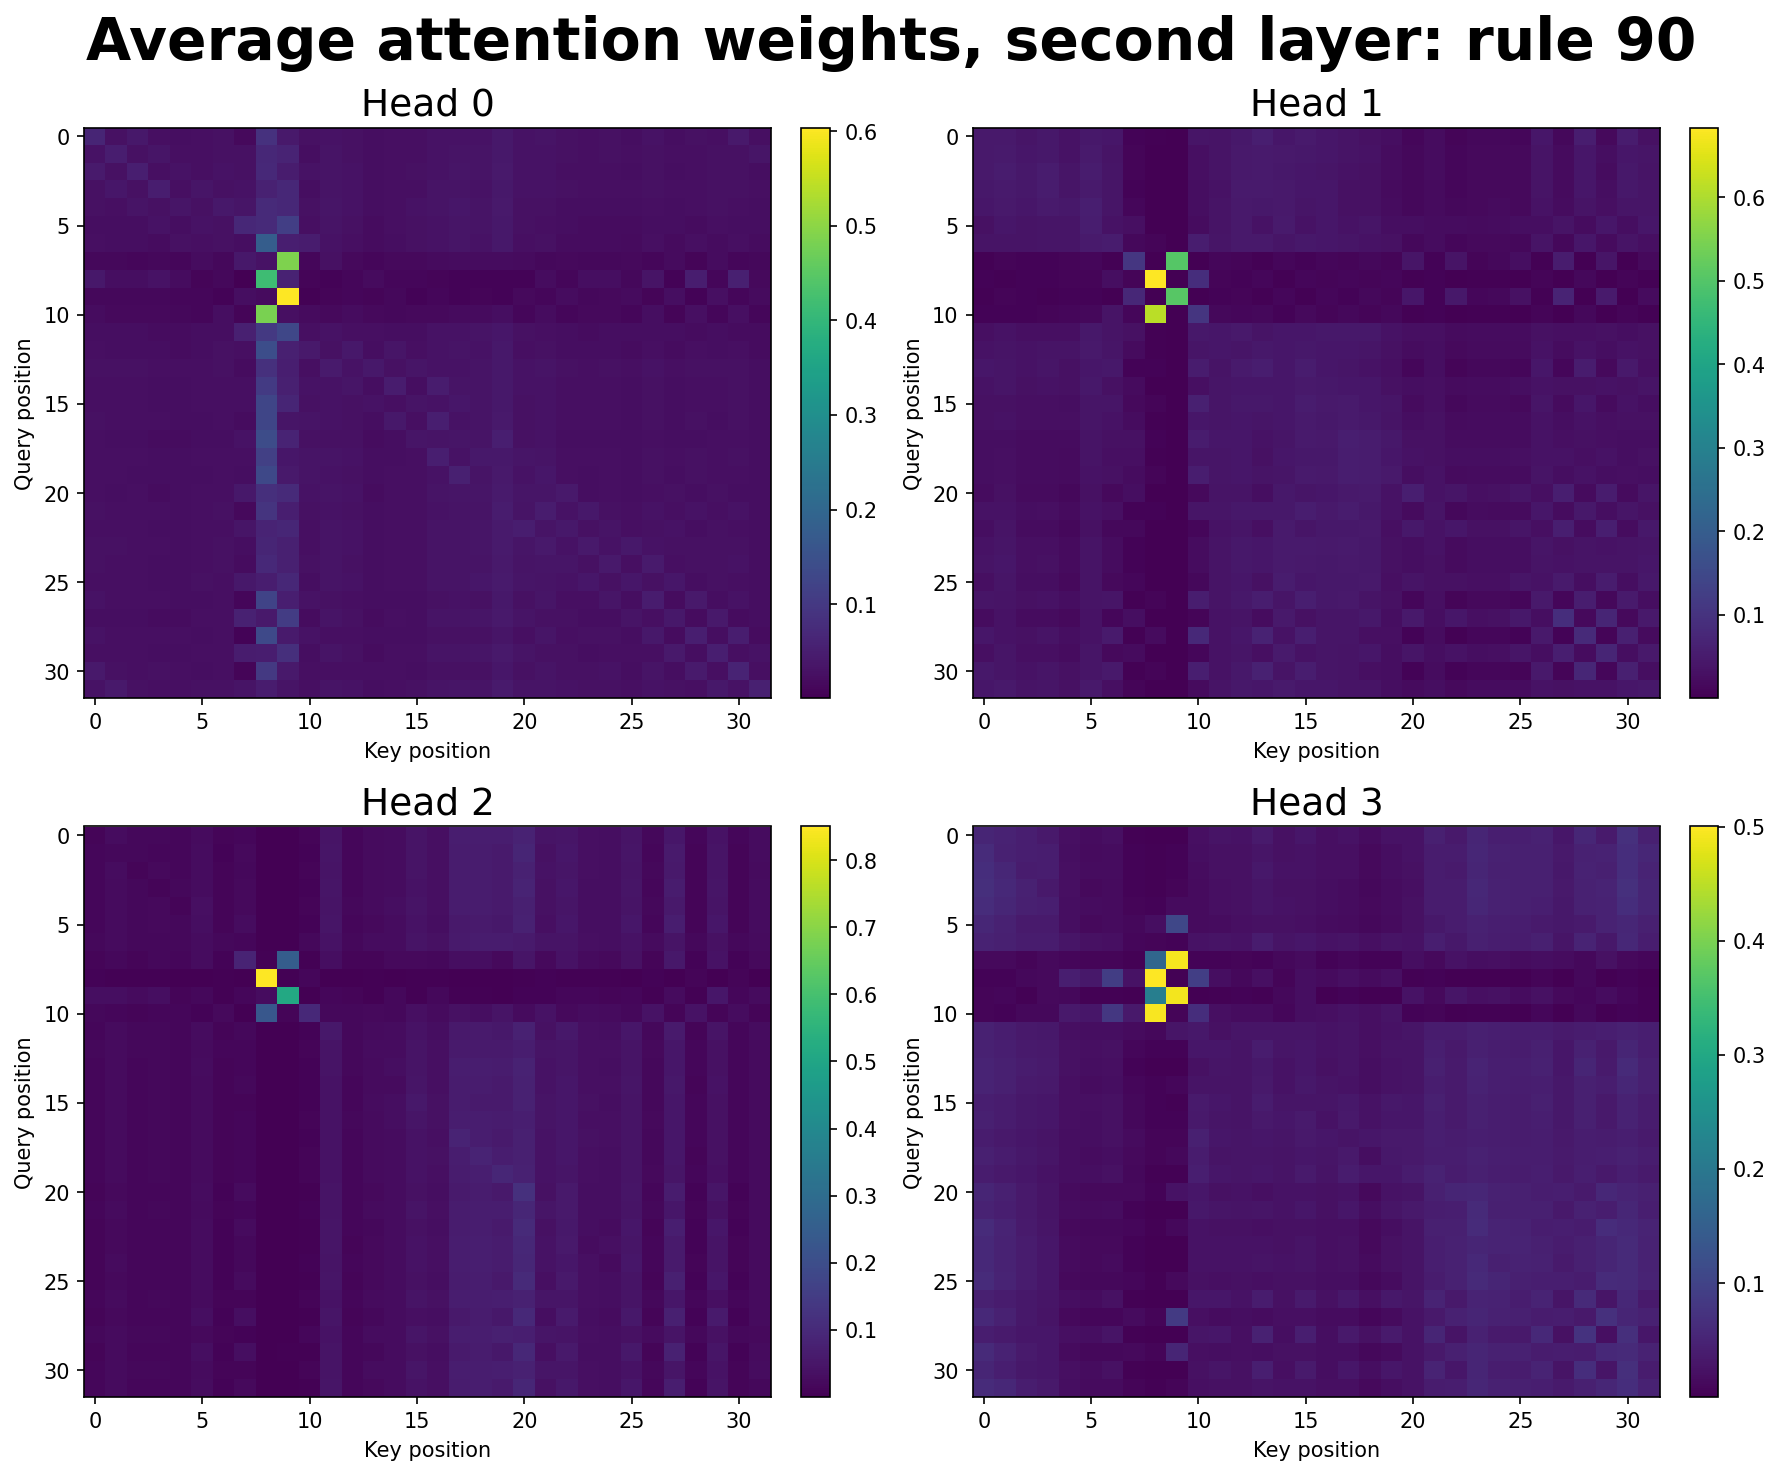
\includegraphics[width=0.45\linewidth]{../results/first_experiment/attention_layer_1_rule_90.png} \\
    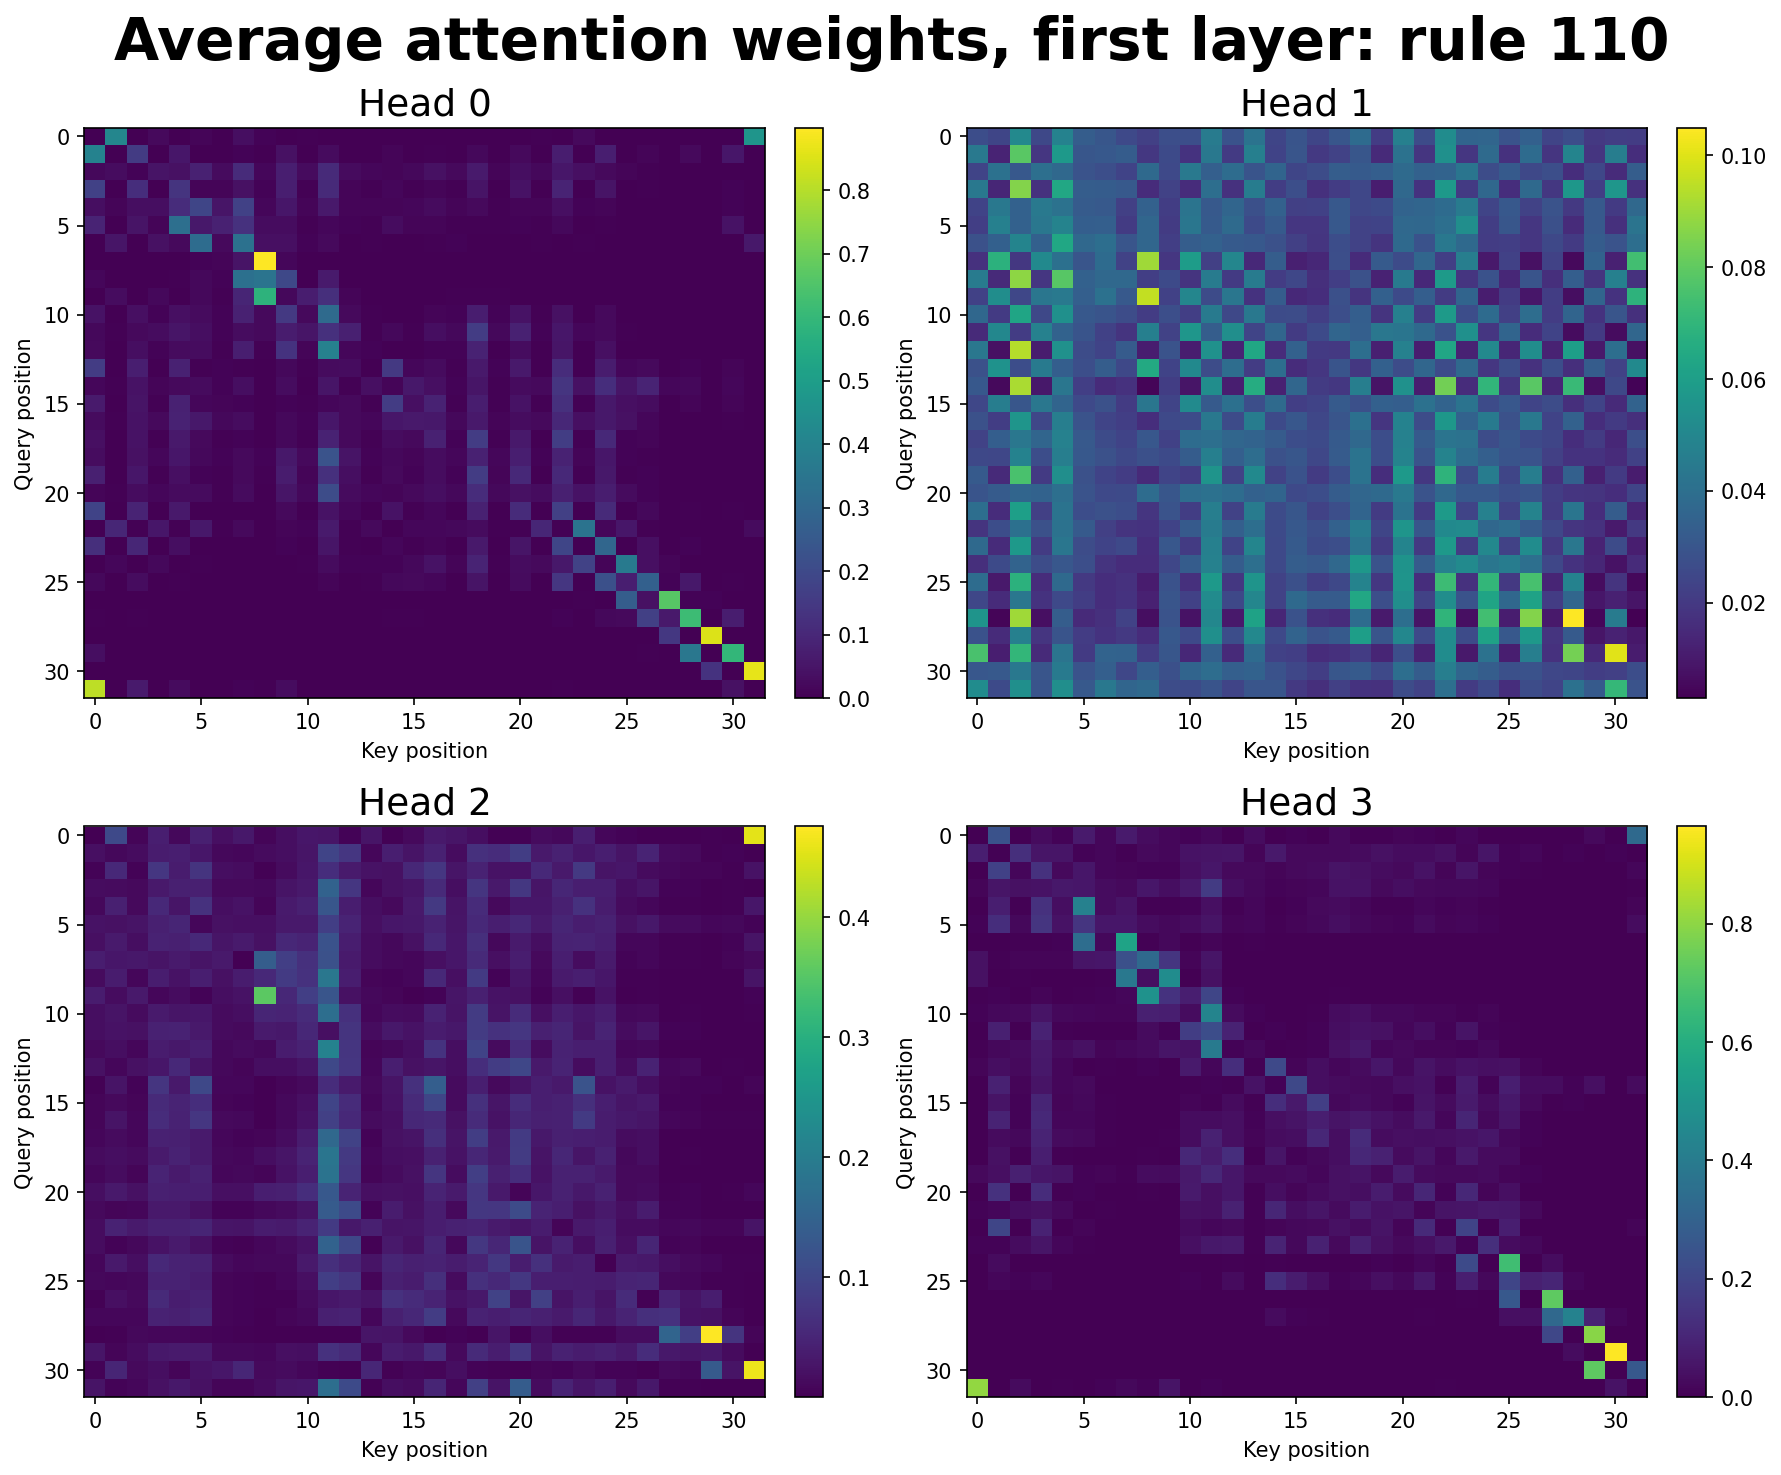
\includegraphics[width=0.45\linewidth]{../results/first_experiment/attention_layer_0_rule_110.png}
    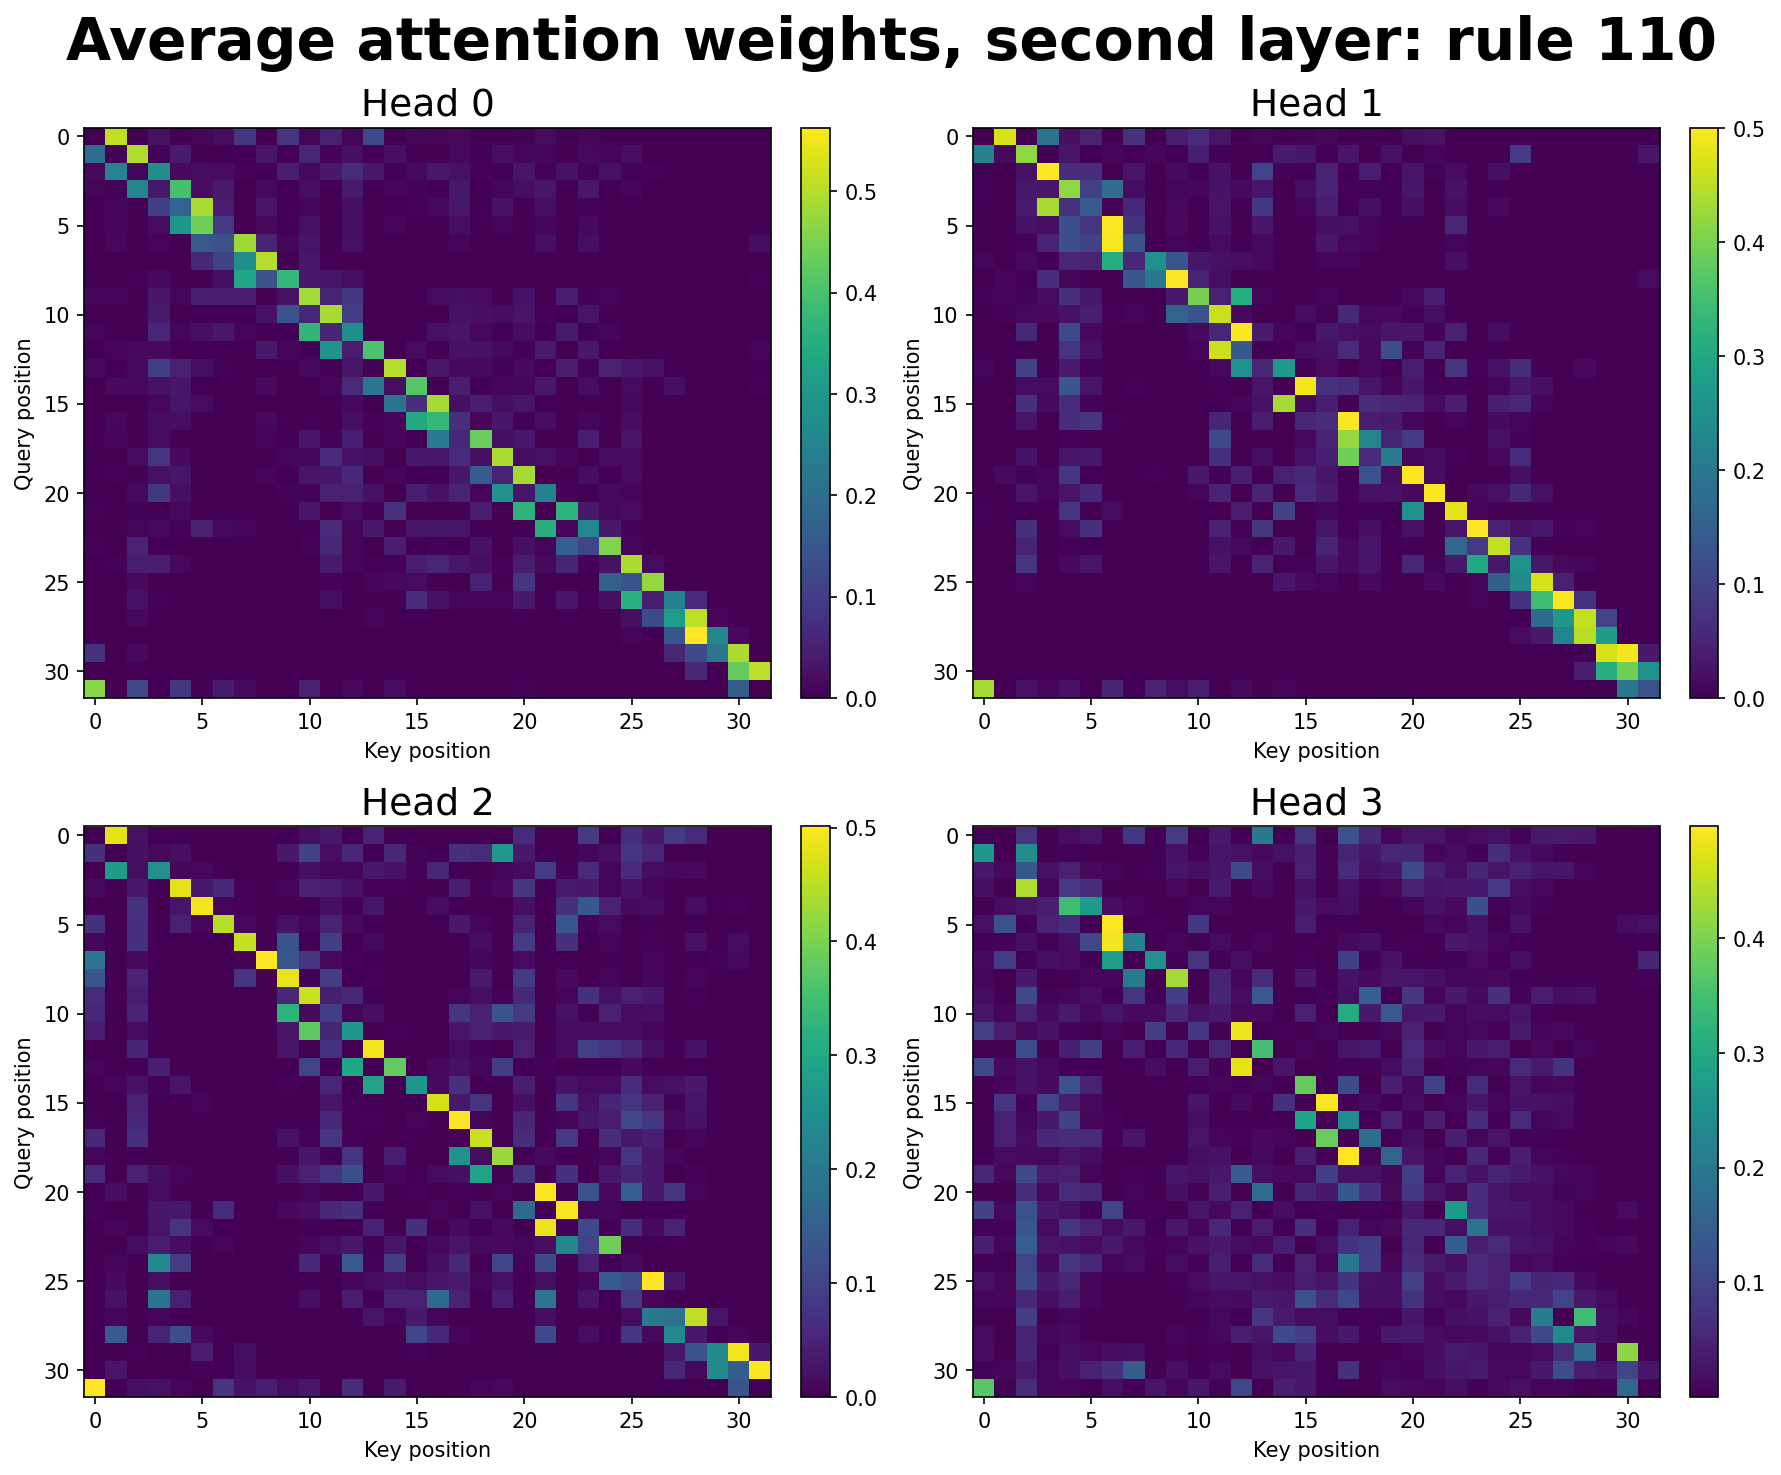
\includegraphics[width=0.45\linewidth]{../results/first_experiment/attention_layer_1_rule_110.png} \\
    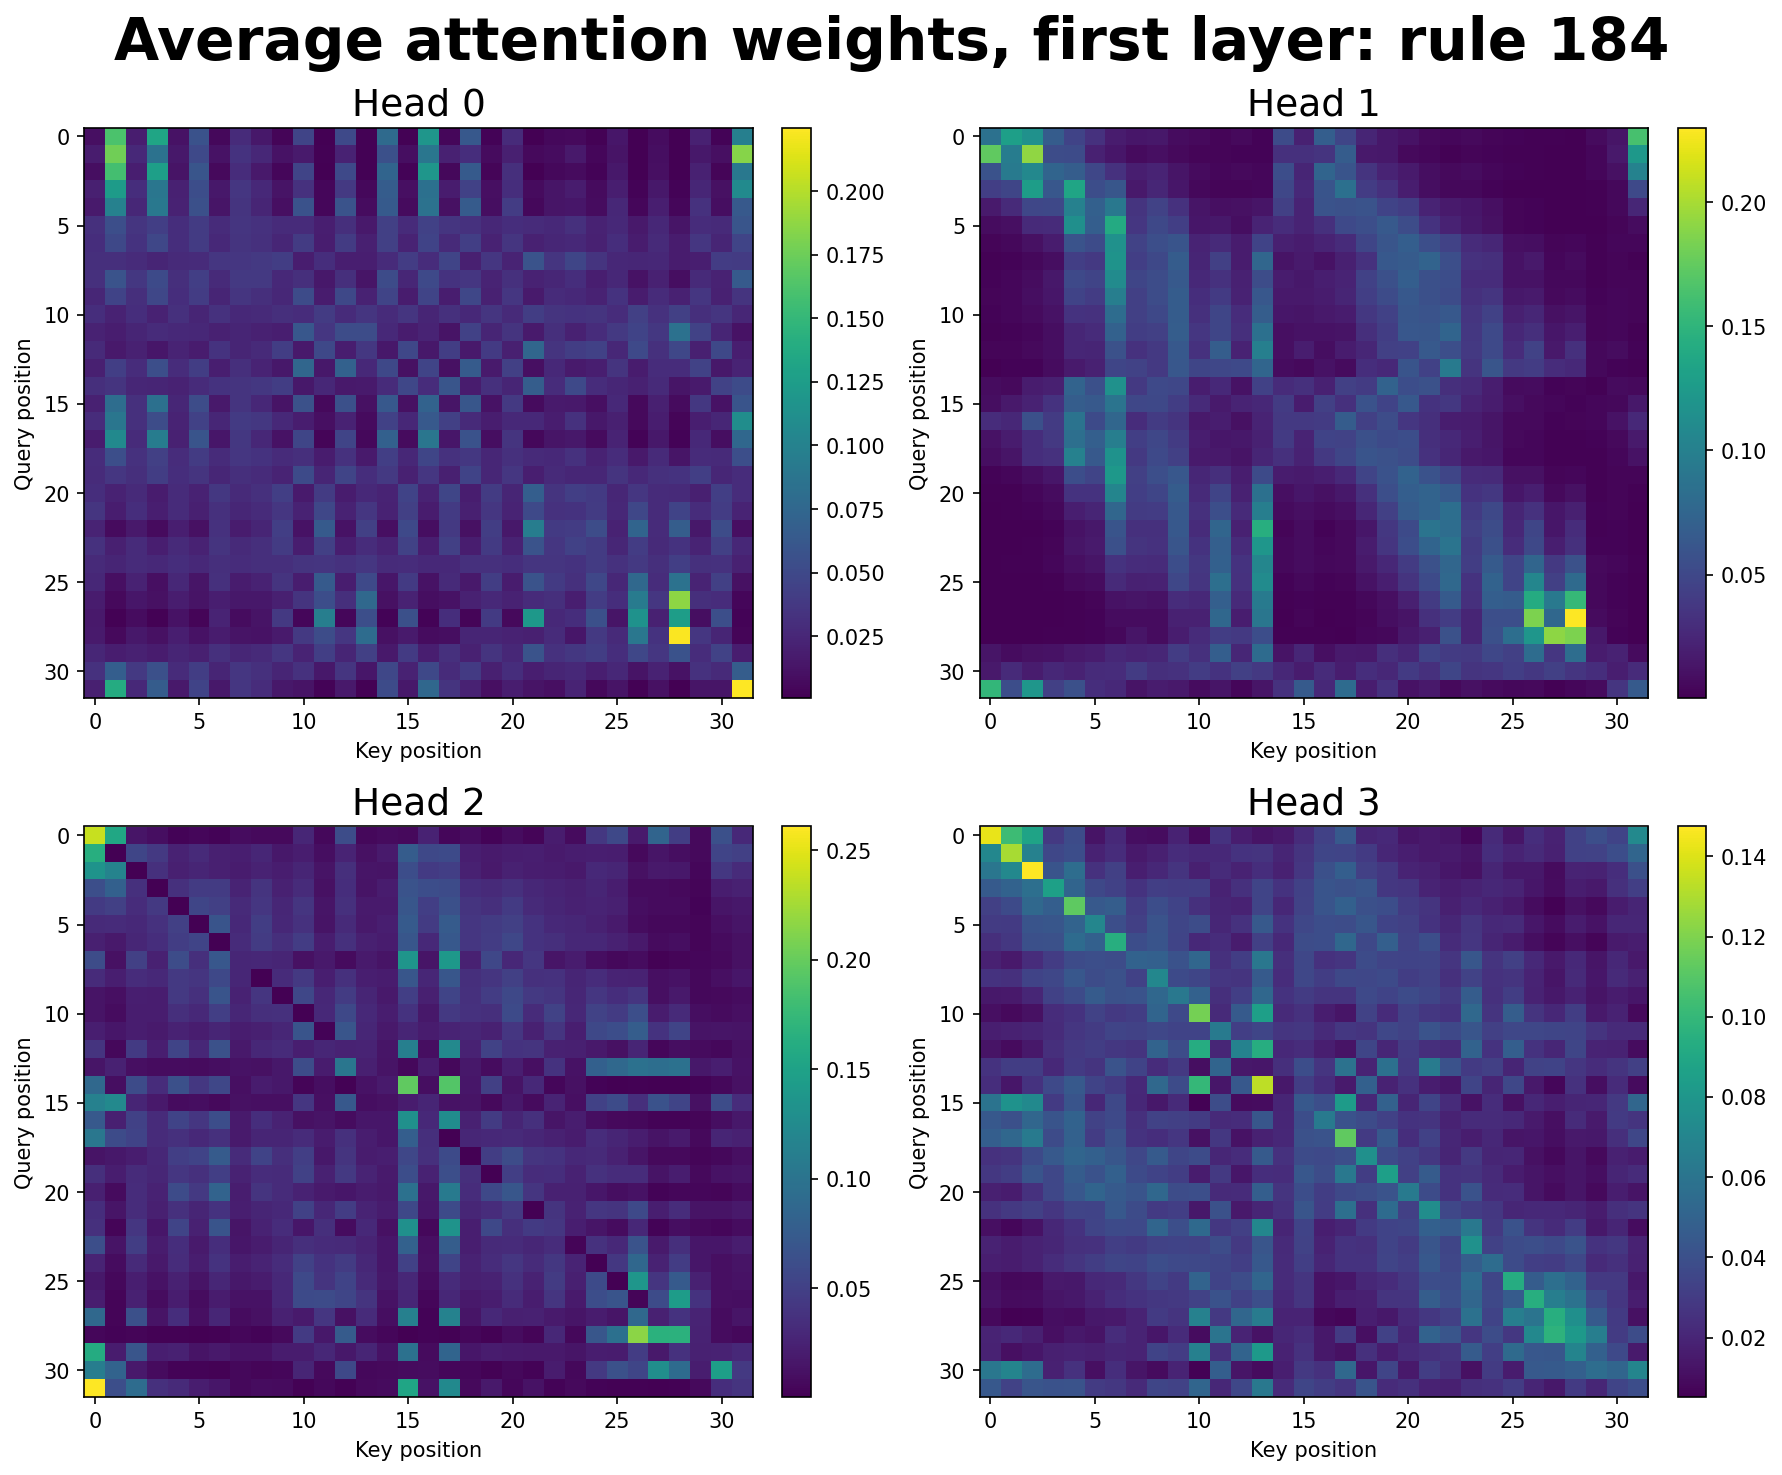
\includegraphics[width=0.45\linewidth]{../results/first_experiment/attention_layer_0_rule_184.png}
    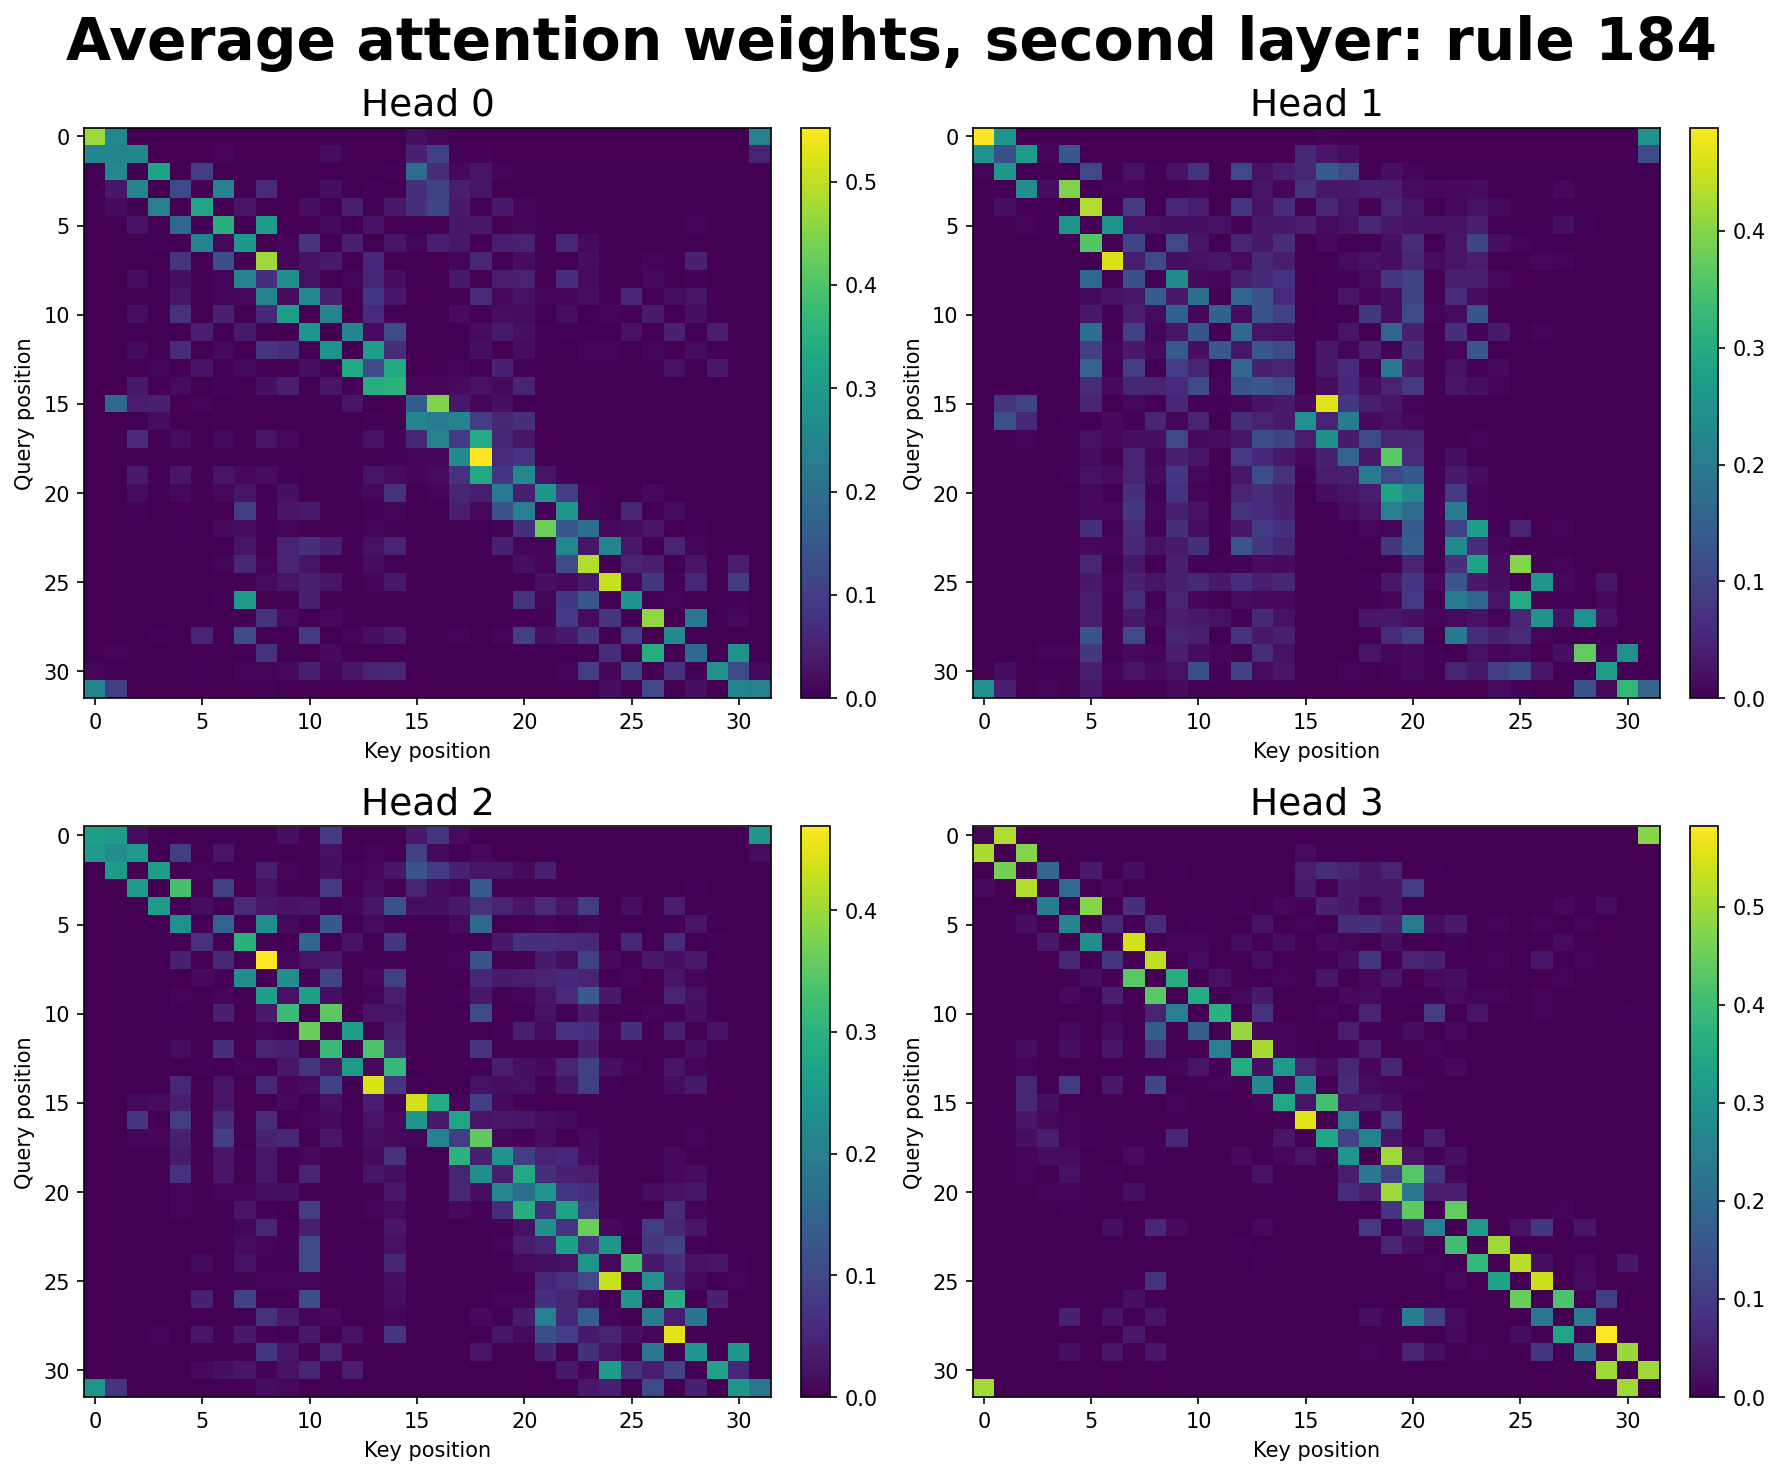
\includegraphics[width=0.45\linewidth]{../results/first_experiment/attention_layer_1_rule_184.png}
    \caption{Attention weights for both layer (first layer left, second layer right): from top to bottom, Rule 30, Rule 90, Rule 110, Rule 184. Each image shows the average attention weights across all test samples.}
    \label{fig:attention}
\end{figure}


\section{Generalization to Longer Sequences}
\label{sec:generalization}

In the second part of the project, we investigate the model's ability to generalize, both to longer sequences and to multiple steps prediction. For the first experiment, we had a fixed sequence length $W = 32$ with a learnable positional embedding. In order to support variable sequence lengths, we switch to other positional embedding schemes:

\begin{itemize}
    \item \textbf{Sinusoidal positional embedding} (mentioned in \cite{attention-is-all-you-need}) -- An absolute positional embedding (APE) that uses deterministic sine and cosine functions to generate position vectors.
    \item \textbf{Rotary Positional Embedding} (RoPE)~\cite{rope} -- A method that applies a rotation to the query and key vectors in the attention mechanism based on their position.
\end{itemize}

Both of these embedding schemes do not use learnable parameters, allowing to process sequences of longer lengths than those seen during training.


\subsection{Sinusoidal Positional Embedding}
\label{sec:sinusoidal}

Sinusoidal embedding is, same as the learnable embedding, an absolute positional embedding (APE). This means that the positional embedding is added to the token embedding before being fed into the Transformer layers. Hence, switching to the other embedding does not require any major changes to the model architecture.

We use the same model's hyperparameters as in the first experiment. We trained the model on variable-length sequences of width $W \in \langle 16, 128 \rangle$ in an attempt to encourage the model to learn a more generalizable solution. We then evaluate the model on sequences of widths $W \in \{ 16, 32, ..., 256 \}$.

The results were quite surprising -- for Rules 30, 110, and 184, the model trained well, still achieving perfect accuracy on the test set. However, Rule 90 did not converge at all, with the training loss remaining at around $\ln(2)$ and the accuracy metrics staying at around 50\%, which is equivalent to random guessing. Training loss and evaluation metrics history for all four rules are shown in \cref{fig:loss-history-sinusoidal} and \cref{fig:eval-history-sinusoidal}.

\begin{figure}[ht]
    \centering
    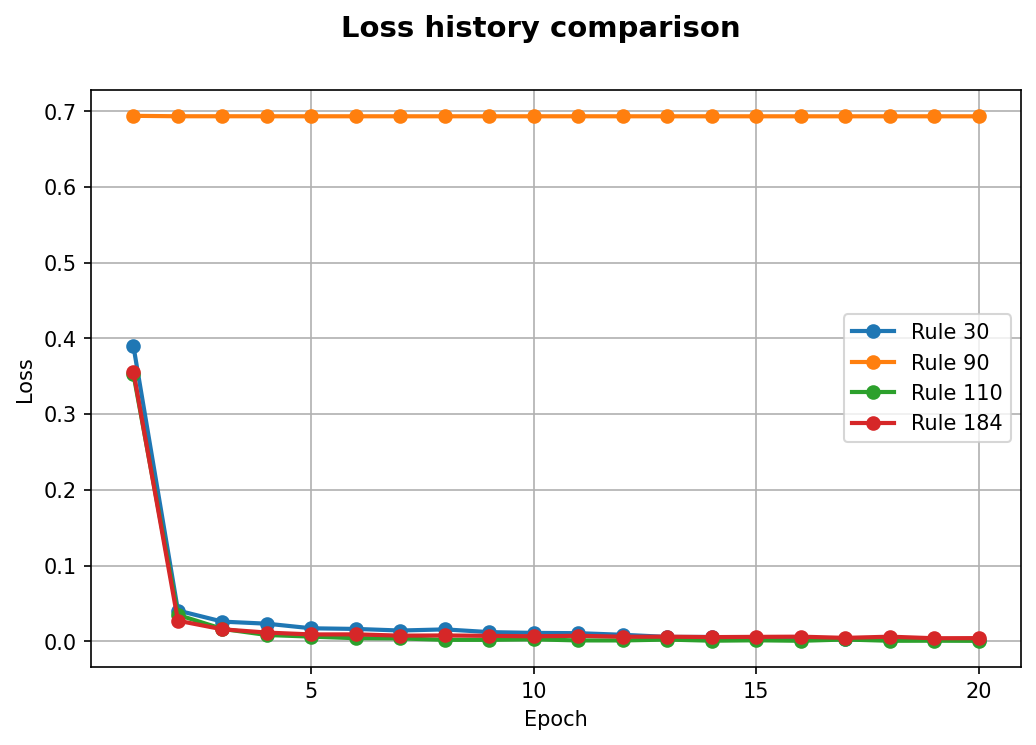
\includegraphics[width=\linewidth]{../results/generalize_length_sinusoidal/loss_history_comparison.png}
    \caption{Training loss comparison across all four rules with sinusoidal positional embedding.}
    \label{fig:loss-history-sinusoidal}
\end{figure}

\begin{figure}[ht]
    \centering
    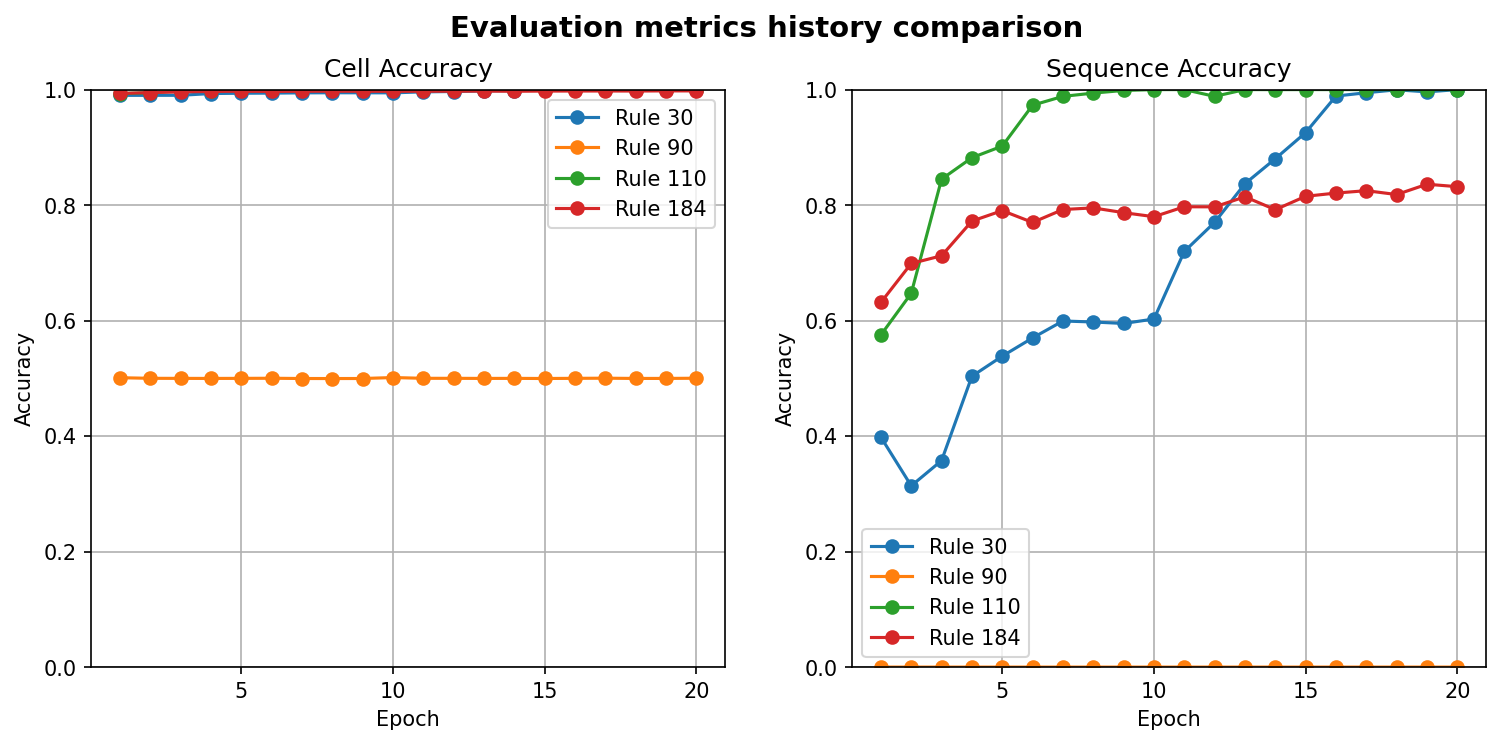
\includegraphics[width=\linewidth]{../results/generalize_length_sinusoidal/eval_history_comparison.png}
    \caption{Evaluation metrics comparison during training with sinusoidal positional embedding: (left) cell-wise accuracy, (right) sequence-wise accuracy.}
    \label{fig:eval-history-sinusoidal}
\end{figure}

Cell accuracy for different sequence lengths is shown in \cref{fig:cell-accuracy-sinusoidal}. It is easy to see that the models (except for Rule 90) have almost perfect accuracy on sequences of lengths seen during training (16 to 128), but for longer sequences, the accuracy gradually drops. The model trained on Rule 90 with sinusoidal positional embedding did not learn anything, hence the cell accuracy is around 50\% for all sequence lengths.

\begin{figure}[ht]
    \centering
        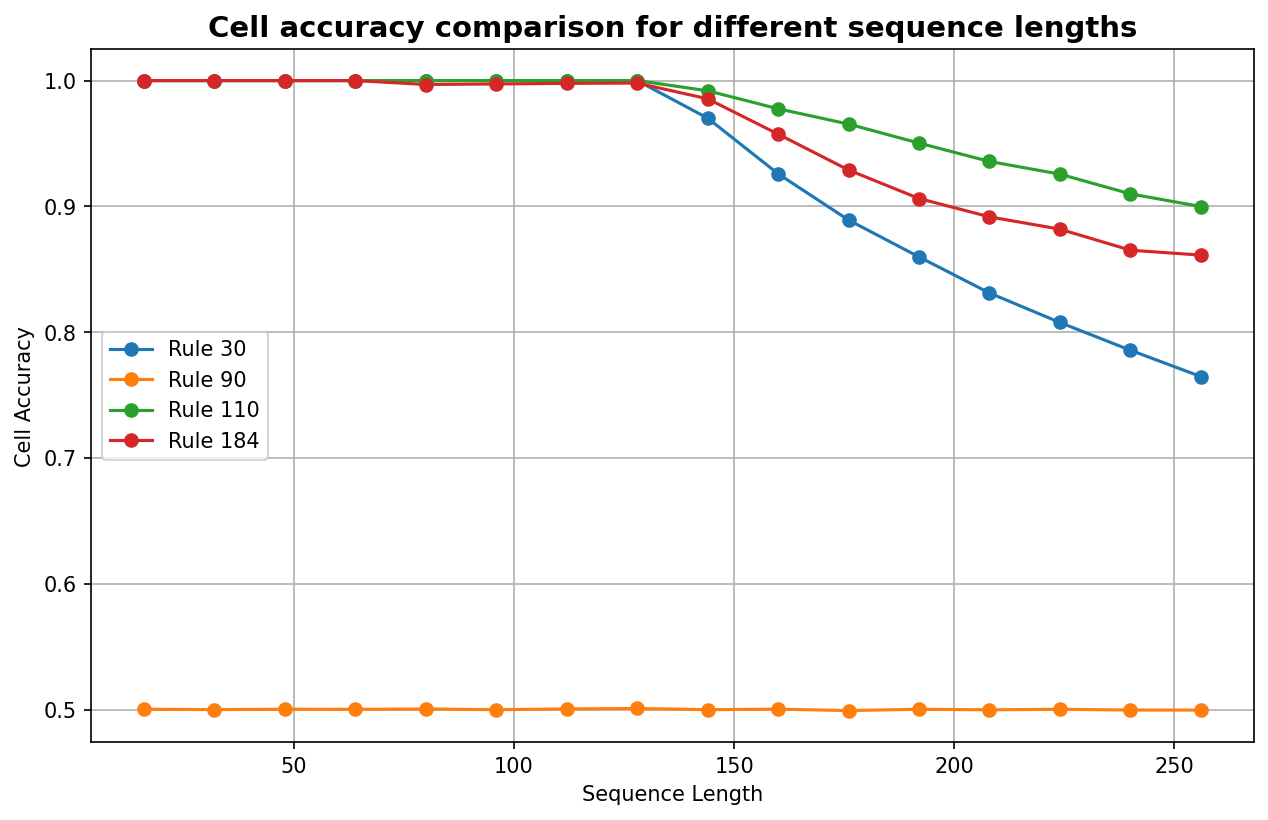
\includegraphics[width=\linewidth]{../results/generalize_length_sinusoidal/cell_accuracy_comparison.png}
        \caption{Cell accuracy evaluated on test sequences of different lengths with sinusoidal positional embedding. Model was trained on lengths $W \in \langle 16, 128 \rangle$ and evaluated on lengths $W \in \{ 16, 32, ..., 256 \}$.}
    \label{fig:cell-accuracy-sinusoidal}
\end{figure}

Additionally, we attempted to train Rule 90 with a smaller learning rate of $3 \cdot 10^{-4}$, dropout probability of $0.0$, and 40 epochs. This helped the model converge, but it did not achieve perfect accuracy like the other rules -- $99.5\%$ cell accuracy and $63.9\%$ sequence accuracy. Loss and evaluation metrics history are shown in \cref{fig:loss-history-sinusoidal-rule90} and \cref{fig:eval-history-sinusoidal-rule90}. Evaluated cell accuracy on the test set is shown in \cref{fig:cell-accuracy-sinusoidal-rule90}. We can see the same drop in accuracy for sequences longer than 128, with sequences of length 256 having around $70\%$ cell accuracy.

\begin{figure}[ht]
    \centering
    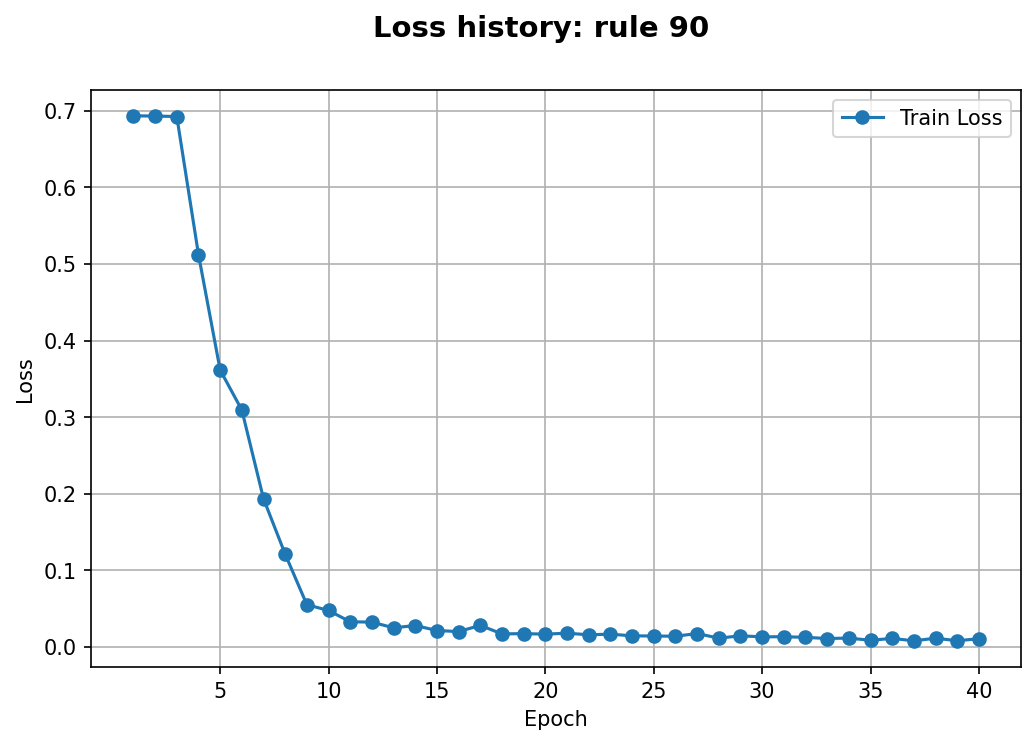
\includegraphics[width=\linewidth]{../results/rule_90/loss_history_rule_90.png}
    \caption{Training loss history for Rule 90 with sinusoidal positional embedding and modified hyperparameters (learning rate $3 \cdot 10^{-4}$, dropout $0.0$, 40 epochs).}
    \label{fig:loss-history-sinusoidal-rule90}
\end{figure}

\begin{figure}[ht]
    \centering
    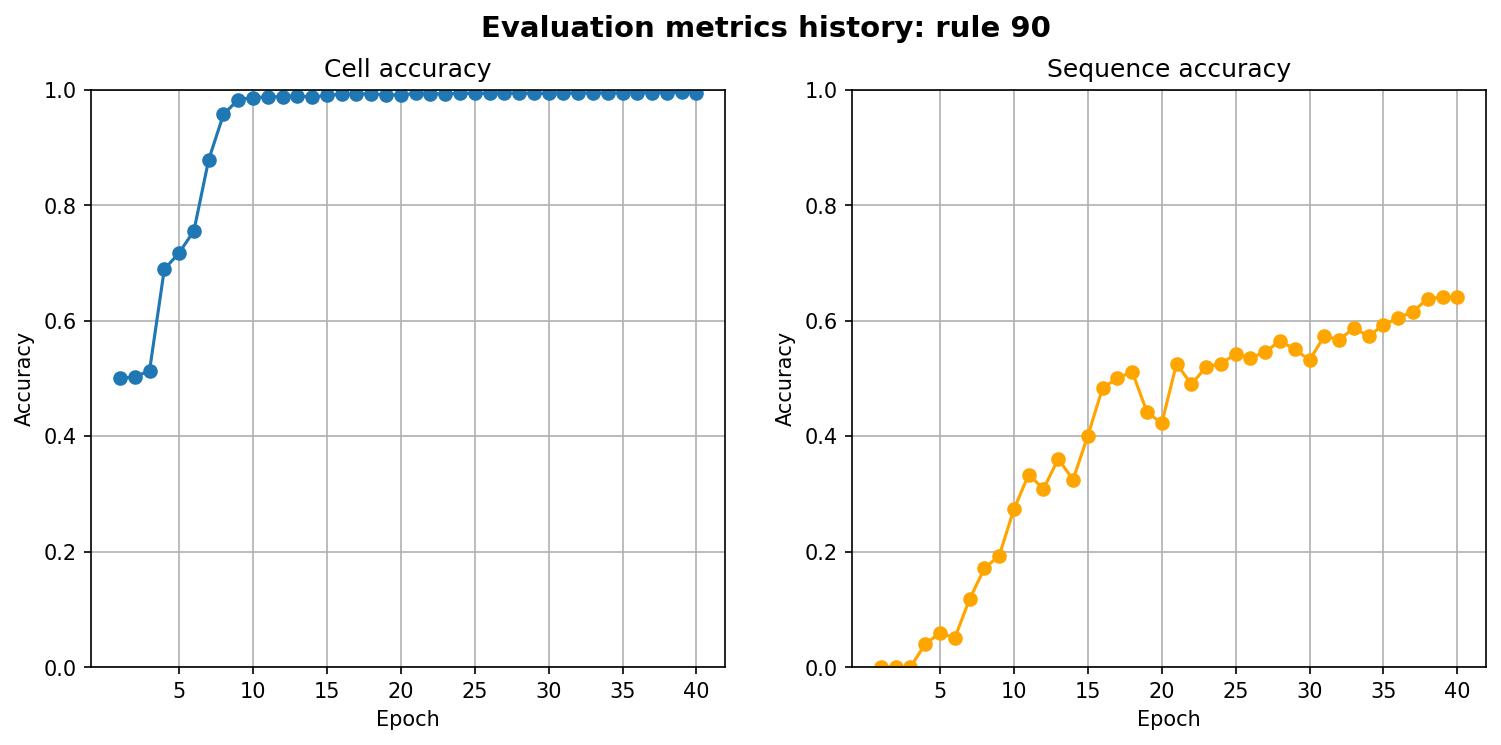
\includegraphics[width=\linewidth]{../results/rule_90/eval_history_rule_90.png}
    \caption{Evaluation metrics history for Rule 90 with sinusoidal positional embedding and modified hyperparameters (learning rate $3 \cdot 10^{-4}$, dropout $0.0$, 40 epochs): (left) cell-wise accuracy, (right) sequence-wise accuracy.}
    \label{fig:eval-history-sinusoidal-rule90}
\end{figure}

\begin{figure}[ht]
    \centering
        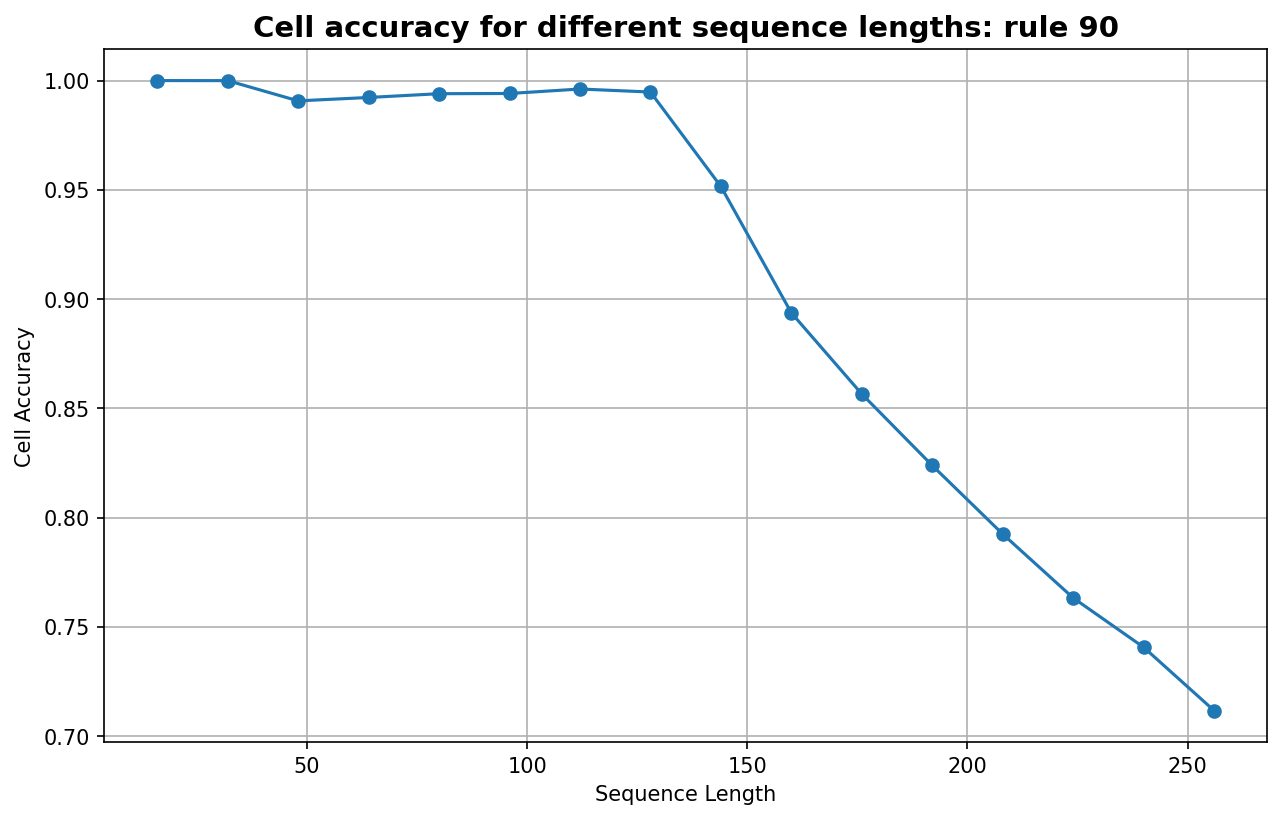
\includegraphics[width=\linewidth]{../results/rule_90/cell_accuracy_rule_90.png}
        \caption{Cell accuracy for Rule 90 with sinusoidal positional embedding and modified hyperparameters (learning rate $3 \cdot 10^{-4}$, dropout $0.0$, 40 epochs) evaluated on test sequences of different lengths.}
    \label{fig:cell-accuracy-sinusoidal-rule90}
\end{figure}


\subsection{Rotary Positional Embedding}
\label{sec:rope}

Rotary Positional Embedding (RoPE) is a relative positional embedding method that applies a rotation to the query and key vectors in the attention mechanism based on their position. Relative positional embeddings are usually superior to absolute ones in terms of generalization to longer sequences and our results support this claim.

We use the same setup as in the sinusoidal embedding experiment, with the same hyperparameters and training on variable-length sequences of width $W \in \langle 16, 128 \rangle$. The training loss and evaluation metrics history are shown in \cref{fig:loss-history-rope} and \cref{fig:eval-history-rope}, while the cell accuracy for different sequence lengths is shown in \cref{fig:cell-accuracy-rope}.

\begin{figure}[ht]
    \centering
    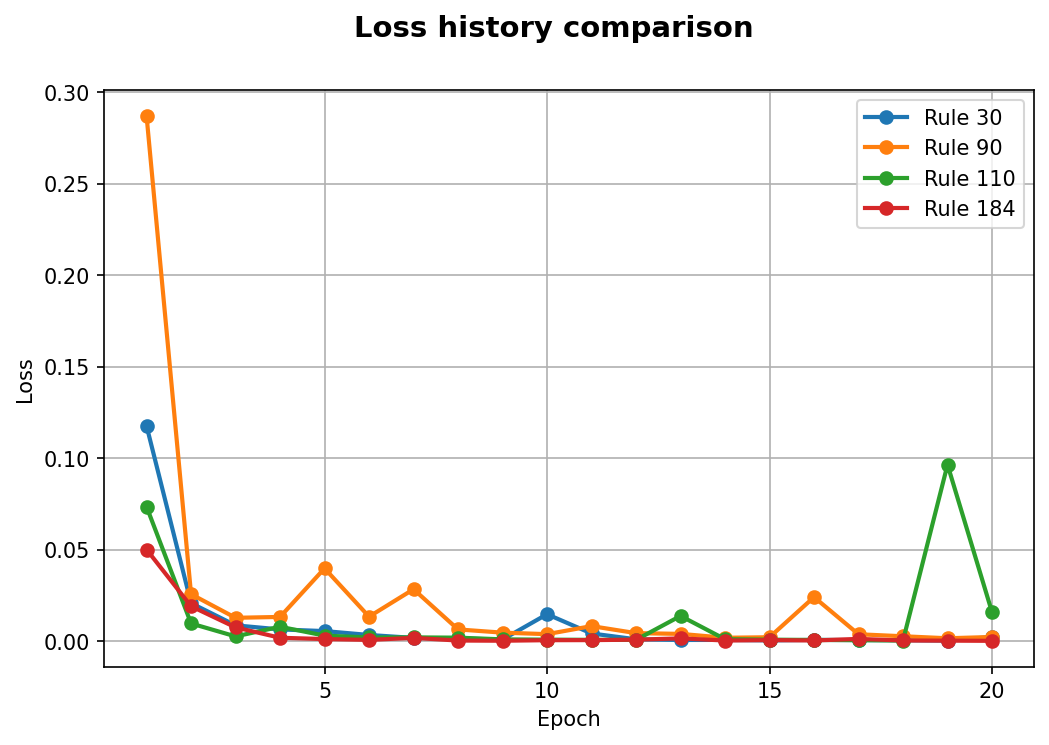
\includegraphics[width=\linewidth]{../results/generalize_length_rope/loss_history_comparison.png}
    \caption{Training loss comparison across all four rules with RoPE.}
    \label{fig:loss-history-rope}
\end{figure}

\begin{figure}[ht]
    \centering
    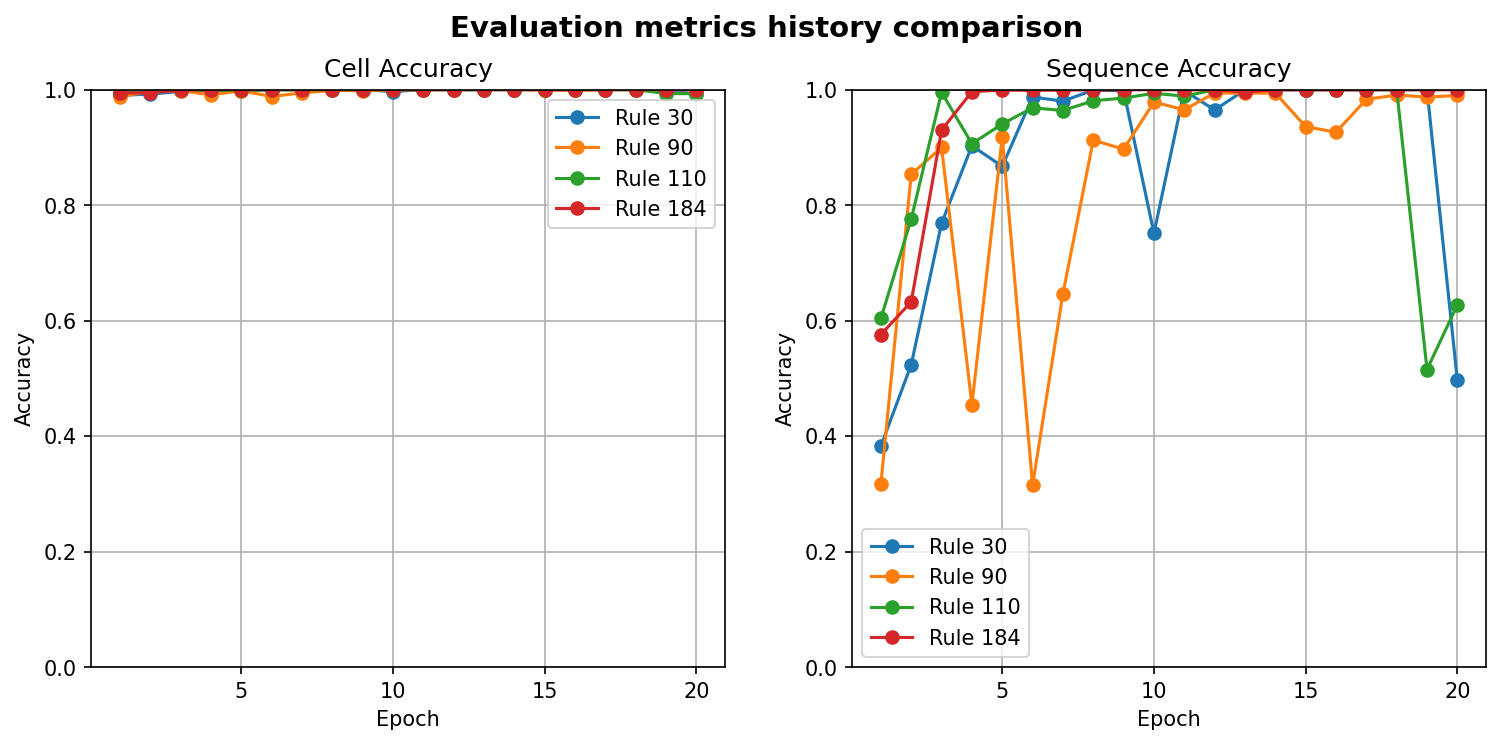
\includegraphics[width=\linewidth]{../results/generalize_length_rope/eval_history_comparison.png}
    \caption{Evaluation metrics comparison during training with RoPE: (left) cell-wise accuracy, (right) sequence-wise accuracy.}
    \label{fig:eval-history-rope}
\end{figure}

\begin{figure}[ht]
    \centering
        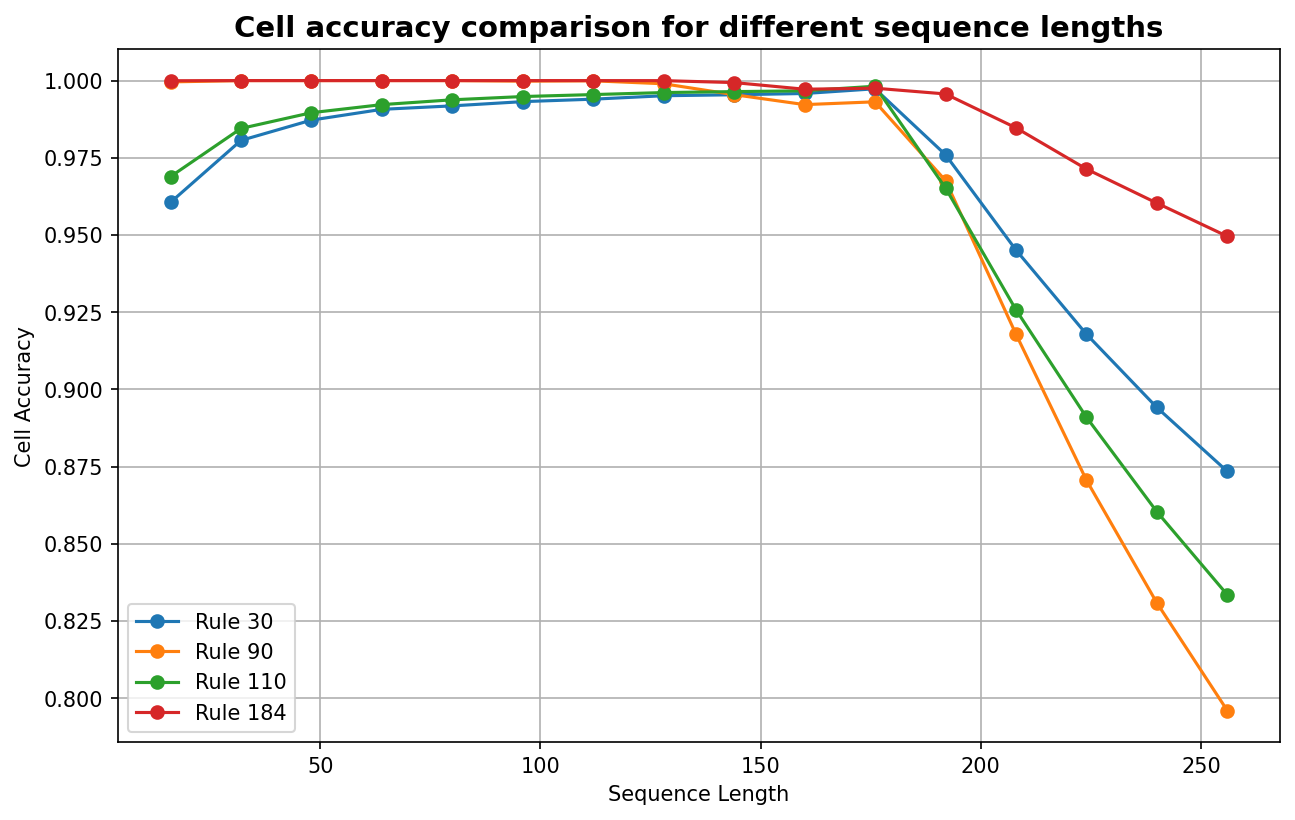
\includegraphics[width=\linewidth]{../results/generalize_length_rope/cell_accuracy_comparison.png}
        \caption{Cell accuracy evaluated on test sequences of different lengths with RoPE. Model was trained on lengths $W \in \langle 16, 128 \rangle$ and evaluated on lengths $W \in \{ 16, 32, ..., 256 \}$.}
    \label{fig:cell-accuracy-rope}
\end{figure}

Compared to the previous experiment, all four rules did generalize better to longer sequences -- accuracy did not drop as soon as the sequence length exceeded 128, but remained high (above $98\%$) up to length 176. However, Rules 30 and 110 show lower cell accuracy on test sequences of short lengths (16 to 48), which is quite surprising, since they were seen during training and achieved perfect accuracy in the previous experiment with sinusoidal embedding. Since evaluated cell accuracy on train sequences during training are almost perfect, this very likely suggests overfitting to the training data. Rule 184 performed the best, while Rule 90 performed the worst once again (but with much less difference compared to other rules than in the previous experiments).

An important observation is that the model's loss appears to drop much faster with RoPE than with other positional embeddings (with the same hyperparameters and training setup), but shows sudden spikes in later epochs, which was not observed with other embeddings. This could indicate that the model is learning a more generalizable solution faster, but it is also more sensitive to overfitting or other optimization issues, such as exploding gradients. Decreasing the learning rate and increasing the number of epochs could potentially help to achieve better results, but we did not have time to experiment with this.


\section{Generalization to Multiple Steps}
\label{sec:multi-step}

Up to this point, we have only focused on the prediction of the very next state. Multiple steps could be predicted by feeding the model's output back as input for the next prediction. However, a more interesting approach is to train the model to predict fixed number of steps ahead directly.

In single-step prediction, the next state of each cell depends only on the the local neighborhood, but when we increase the number of steps, the dependent neighborhood also increases. This should naturally make the task more difficult, especially for rules with more complex dynamics.

We use the same setup as in the first experiment with fixed sequence length of $W = 32$ and learnable positional embedding, but instead of predicting the next state, we train the model to predict the state after $k$ time steps, where $k \in \{ 2, 3, \dots, 8 \}$. For each $k$, we train a separate model for each rule. The training loss and evaluation metrics history for all rules and different values of $k$ are shown in \cref{fig:loss-history-multi-step-1} and \cref{fig:loss-history-multi-step-2}. Test cell accuracy for different values of $k$ is shown in \cref{fig:cell-accuracy-multi-step}. Here we can see that Rule 184 kept high accuracy even for larger values of $k$, while Rules 30 and 110 show a significant drop in accuracy for $k > 5$ (almost dropping to 50\% meaning they did not learn anything).

The most surprising results are again for Rule 90 -- for $k = 1, 2, 4$ and even $8$ it achieved perfect accuracy, while for other values of $k$ it did not learn anything at all. It is quite interesting that the values of $k$ for which the model trained successfully are exactly the powers of 2. It seems as if the states after $2^n$ steps contain some kind of regularity and structure that the model can learn more easily.

\begin{figure}[ht]
    \centering
    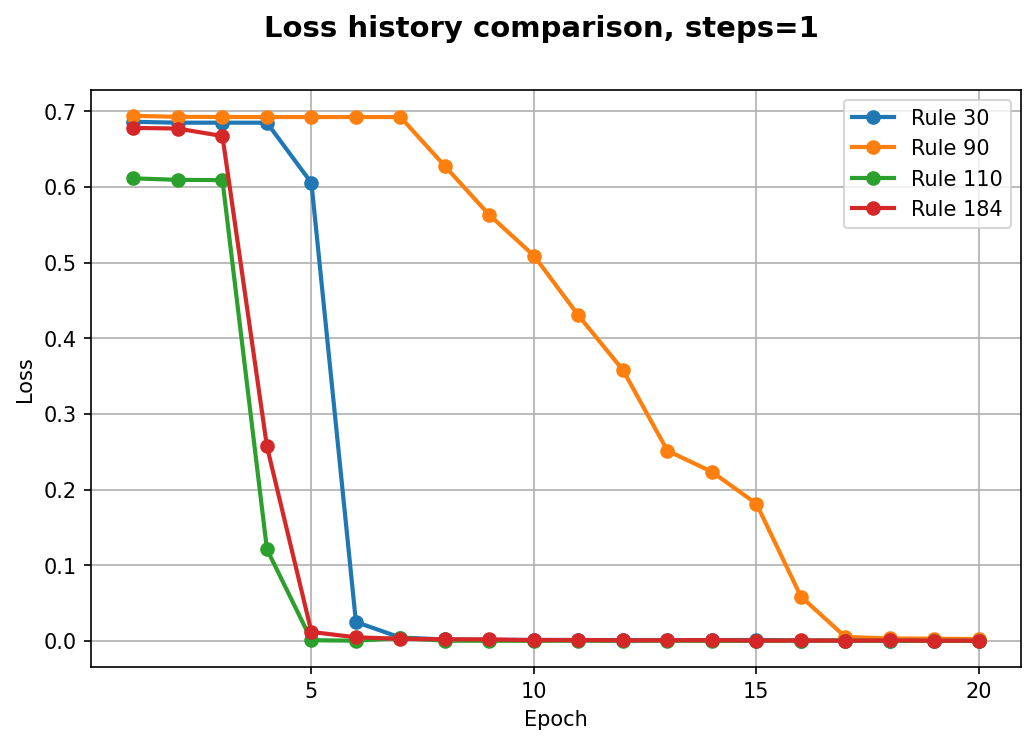
\includegraphics[height=10em]{../results/generalize_steps_1/loss_history_comparison.png}
    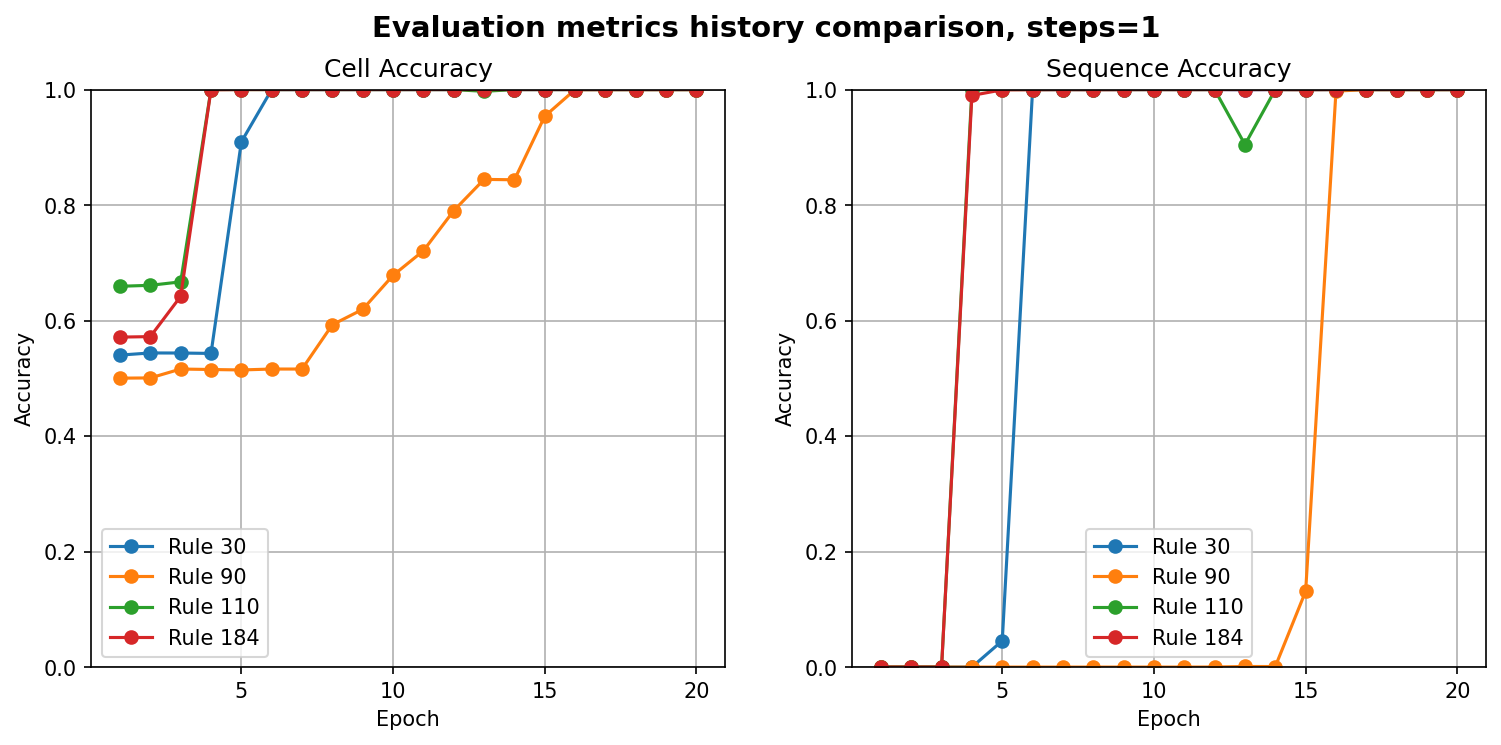
\includegraphics[height=10em]{../results/generalize_steps_1/eval_history_comparison.png}\\
    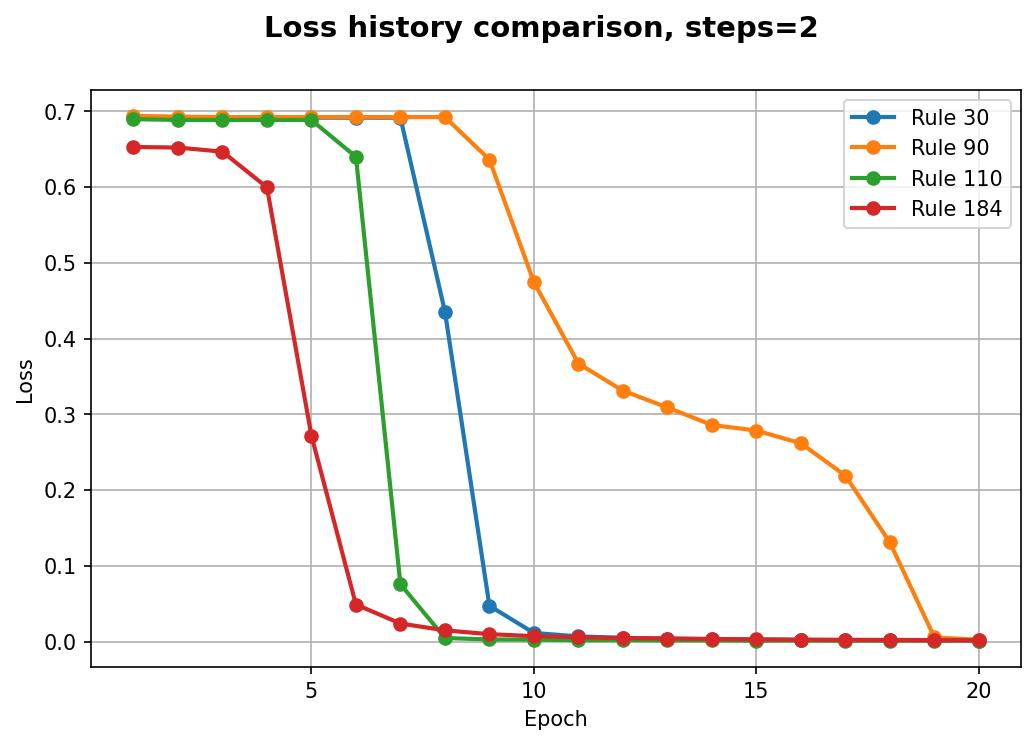
\includegraphics[height=10em]{../results/generalize_steps_2/loss_history_comparison.png}
    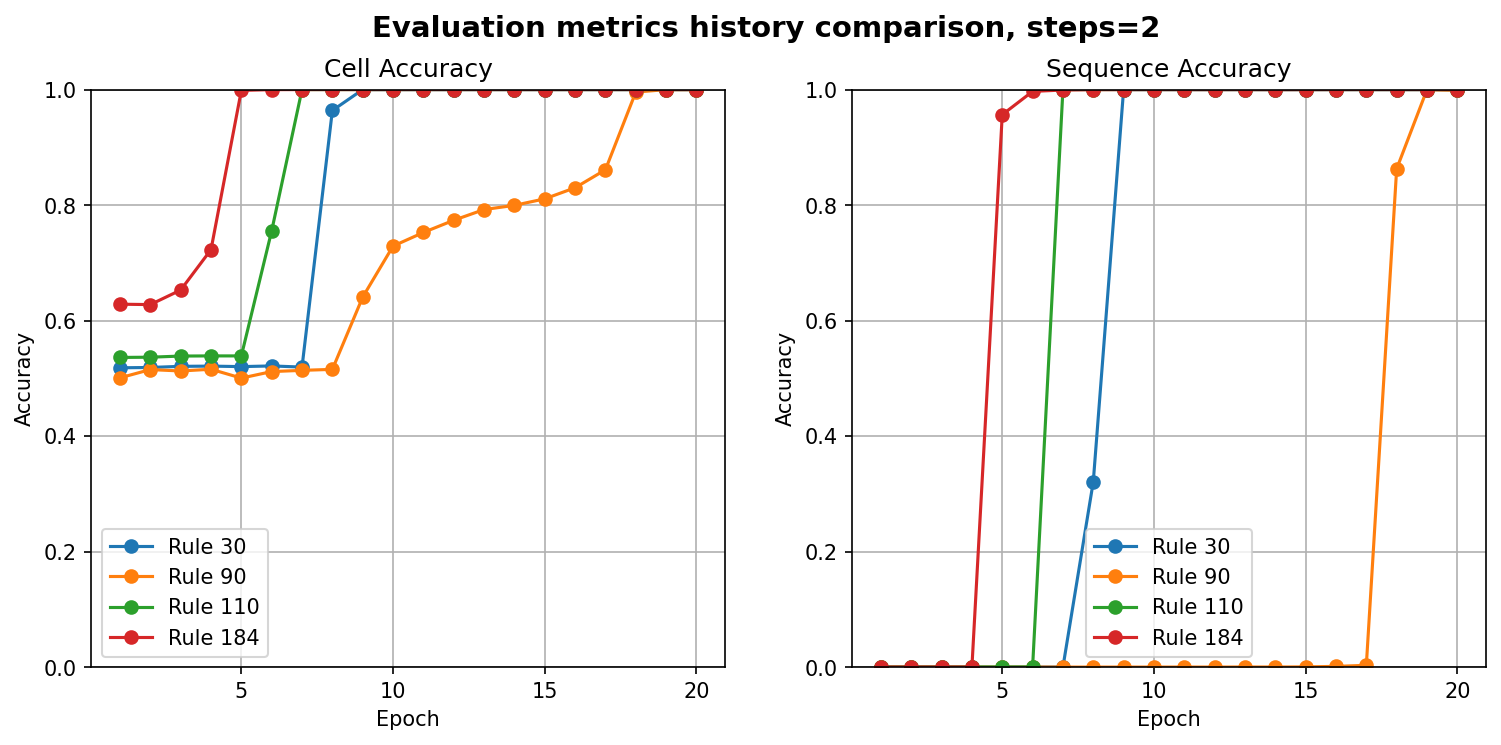
\includegraphics[height=10em]{../results/generalize_steps_2/eval_history_comparison.png}\\
    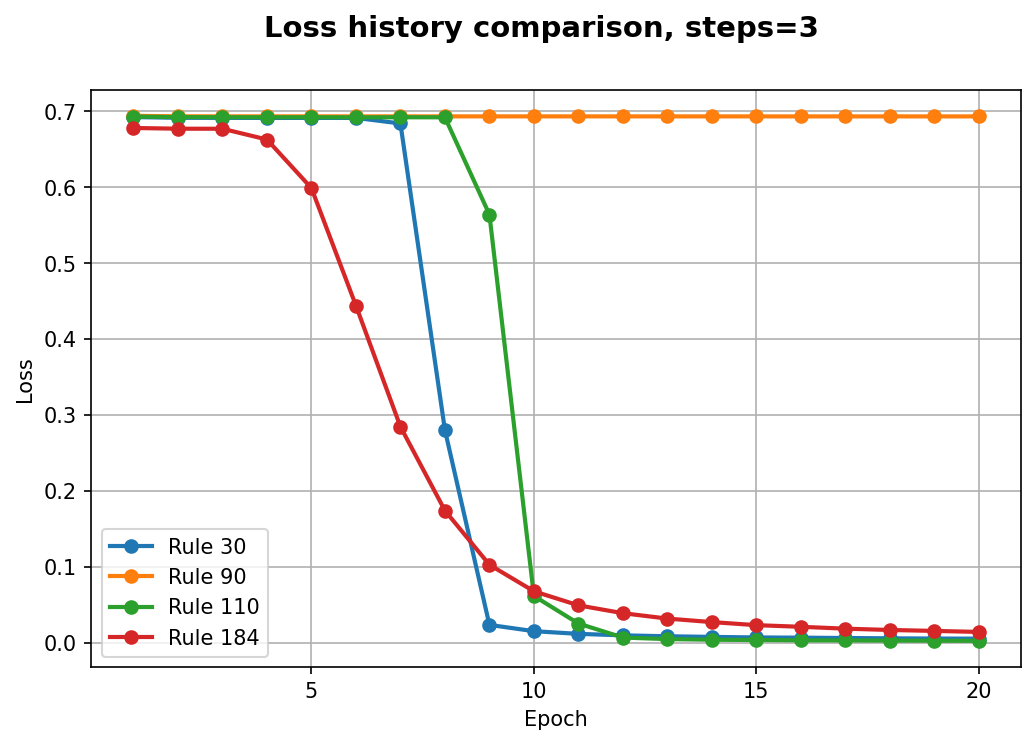
\includegraphics[height=10em]{../results/generalize_steps_3/loss_history_comparison.png}
    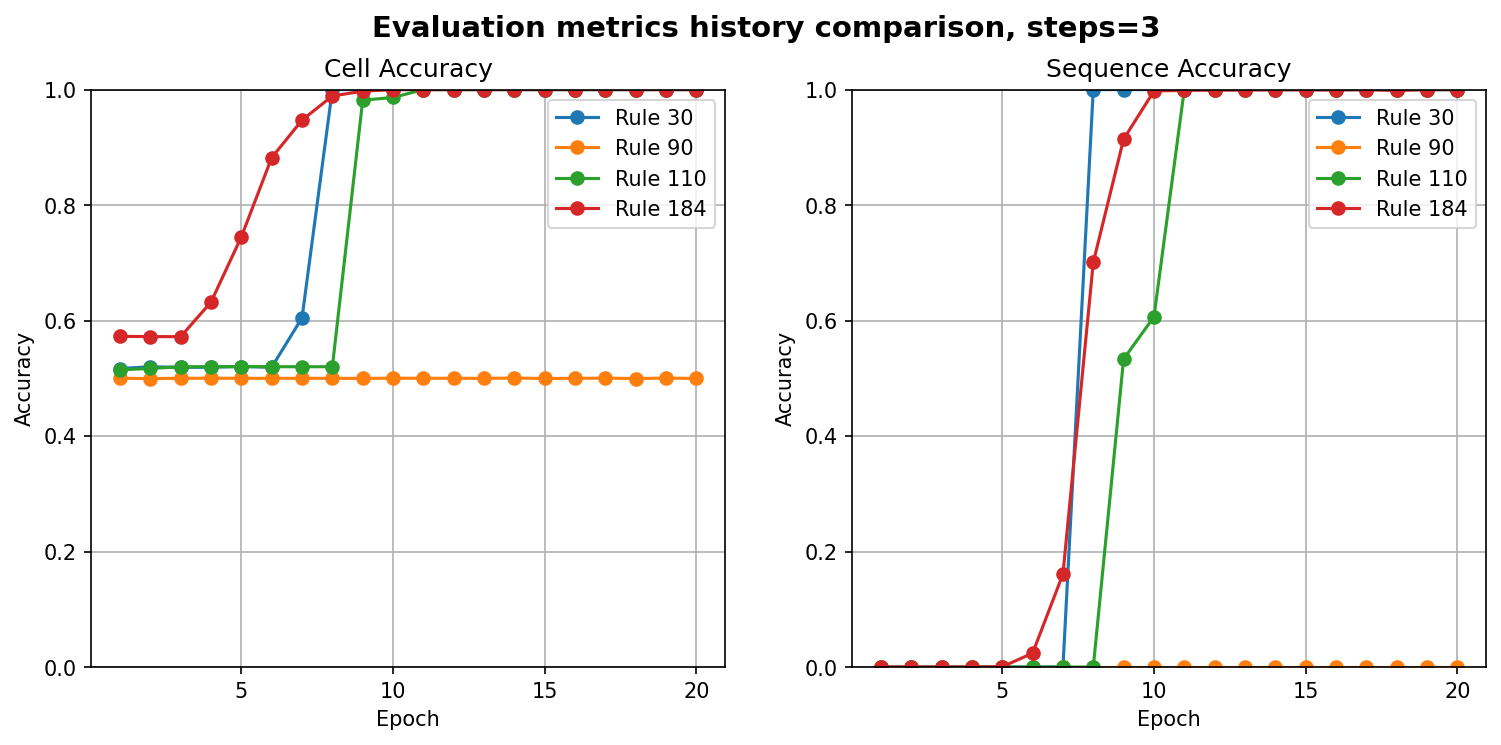
\includegraphics[height=10em]{../results/generalize_steps_3/eval_history_comparison.png}\\
    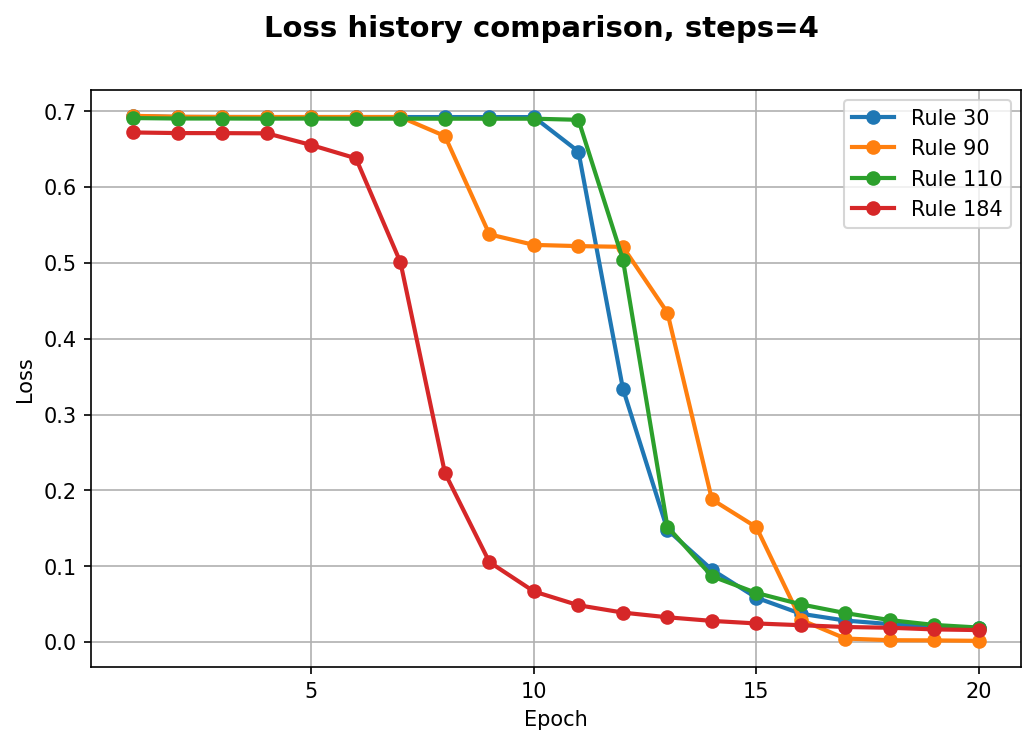
\includegraphics[height=10em]{../results/generalize_steps_4/loss_history_comparison.png}
    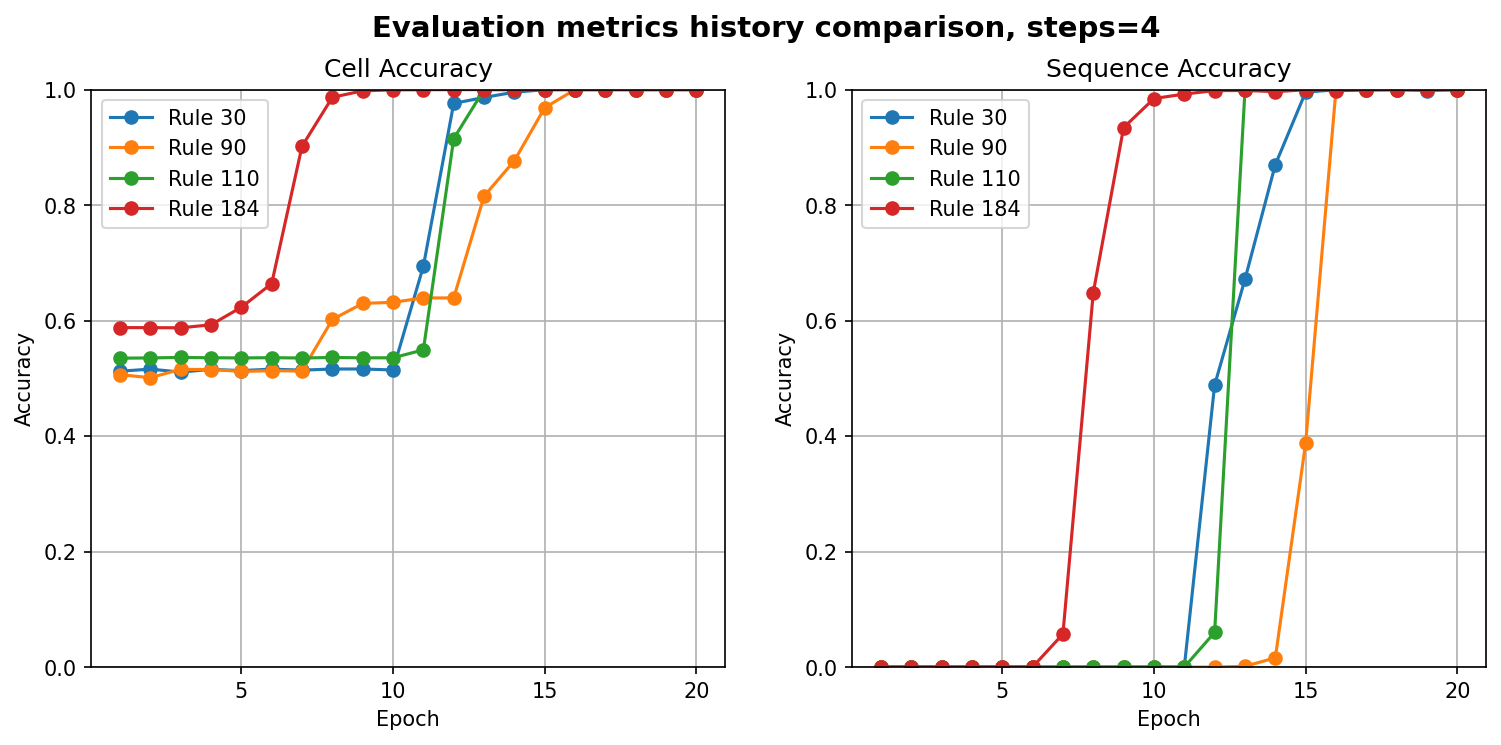
\includegraphics[height=10em]{../results/generalize_steps_4/eval_history_comparison.png}\\
    \caption{Training loss and evaluation metrics history for different number of steps prediction: from top to bottom, $k = 1, 2, 3, 4$.}
    \label{fig:loss-history-multi-step-1}
\end{figure}

\begin{figure}[ht]
    \centering
    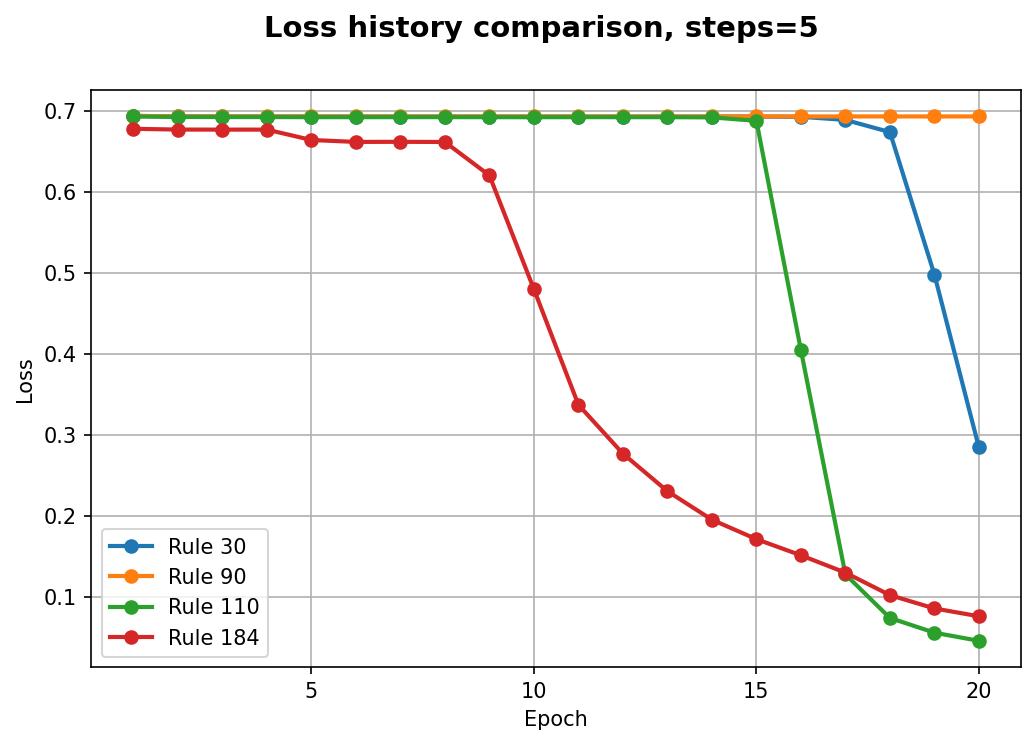
\includegraphics[height=10em]{../results/generalize_steps_5/loss_history_comparison.png}
    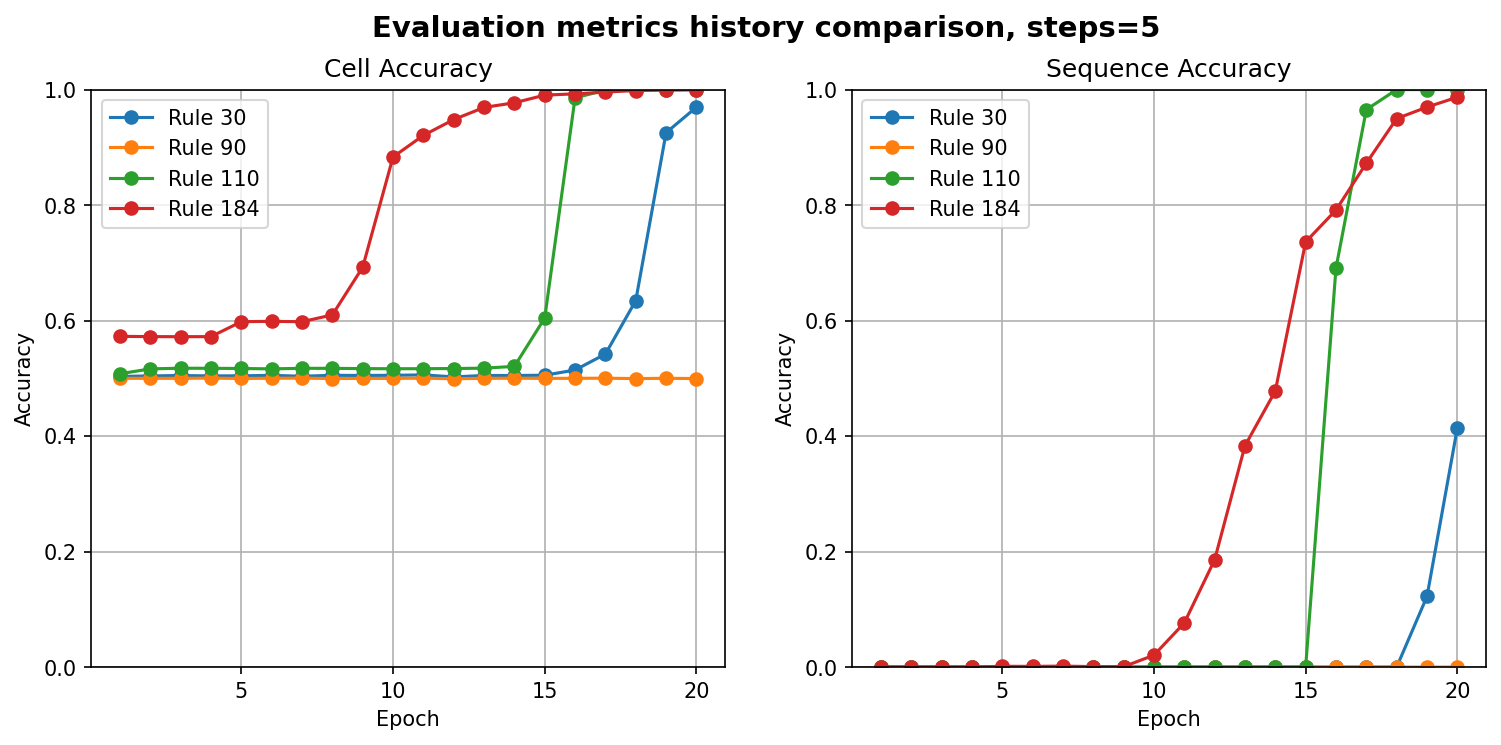
\includegraphics[height=10em]{../results/generalize_steps_5/eval_history_comparison.png}\\
    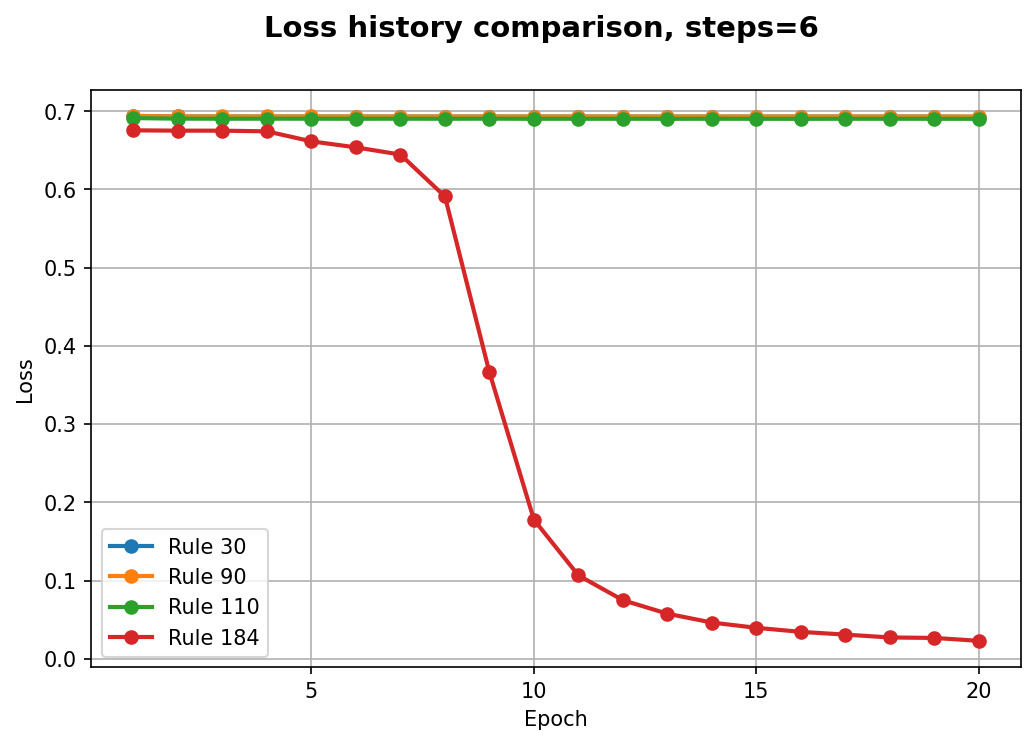
\includegraphics[height=10em]{../results/generalize_steps_6/loss_history_comparison.png}
    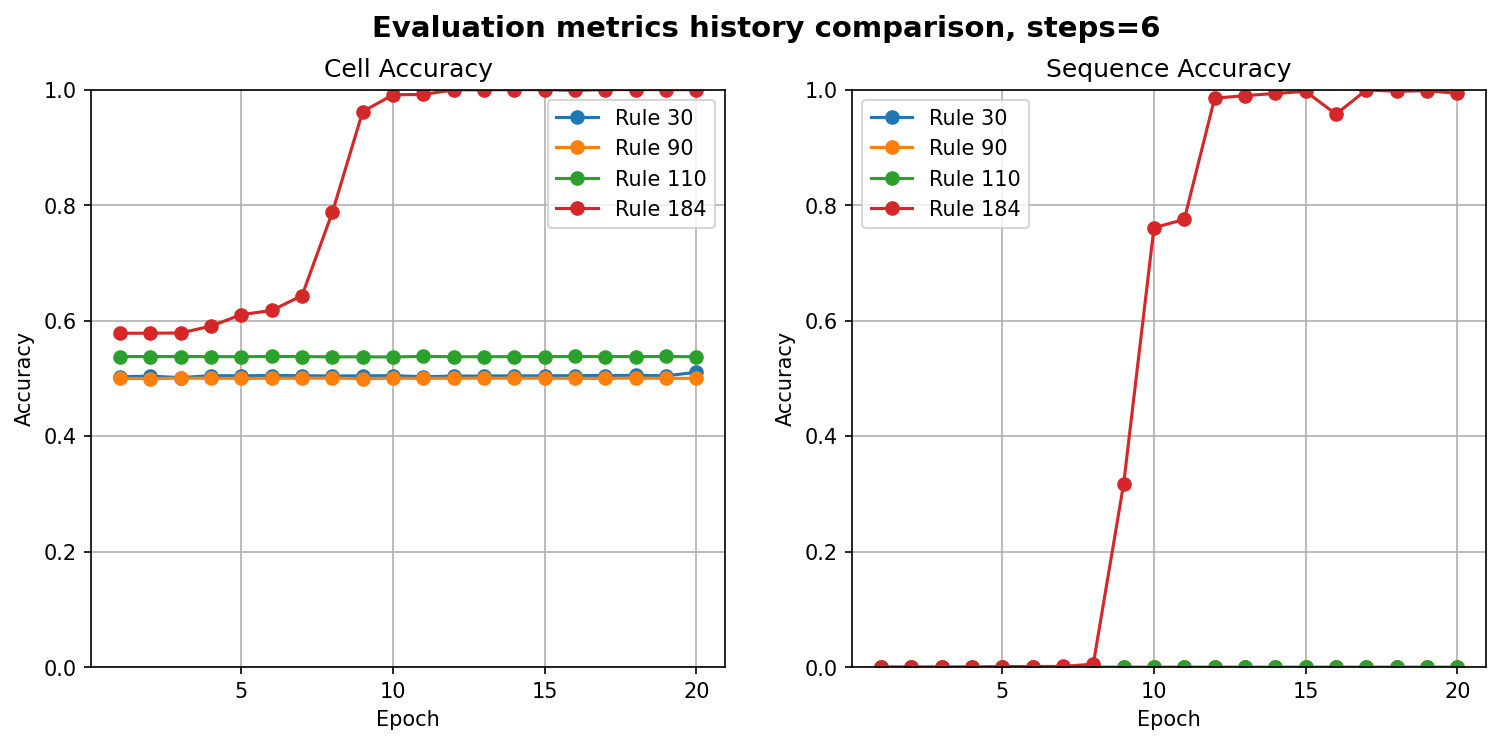
\includegraphics[height=10em]{../results/generalize_steps_6/eval_history_comparison.png}\\
    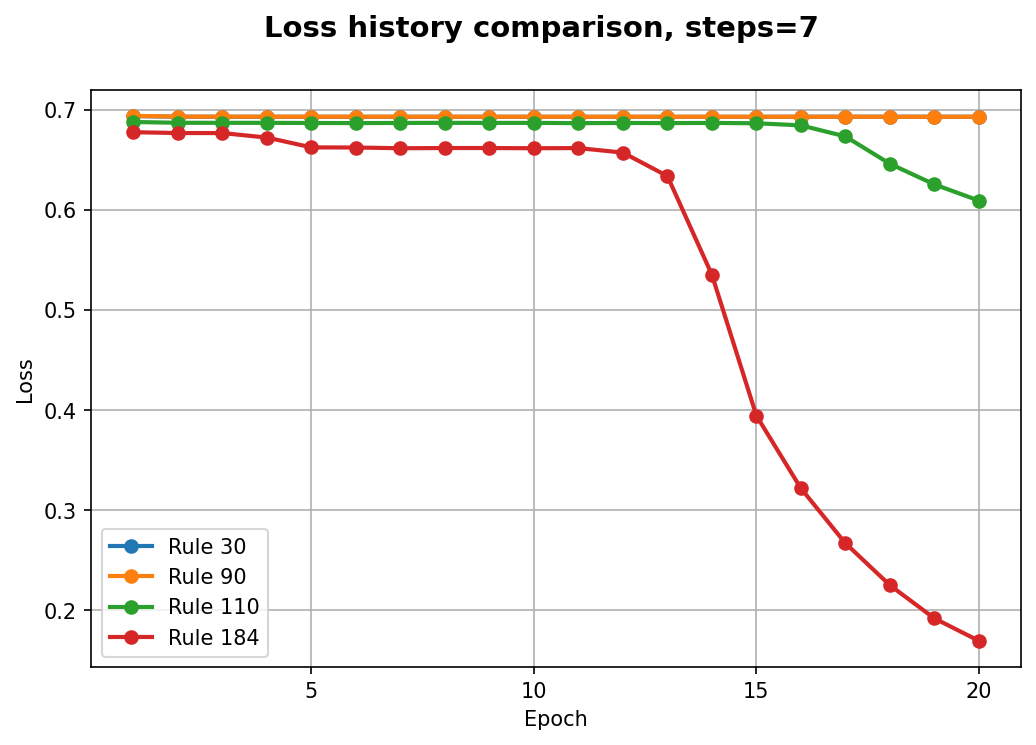
\includegraphics[height=10em]{../results/generalize_steps_7/loss_history_comparison.png}
    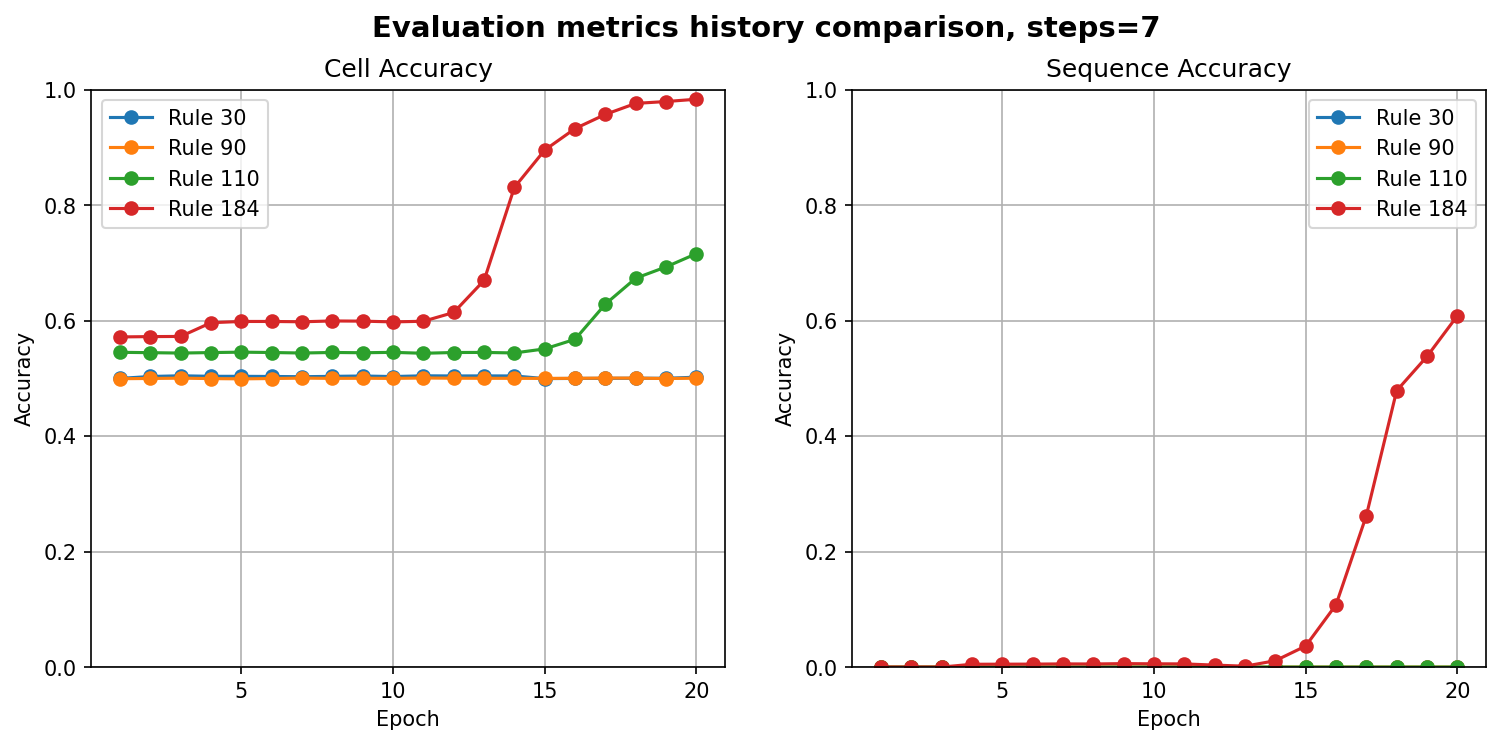
\includegraphics[height=10em]{../results/generalize_steps_7/eval_history_comparison.png}\\
    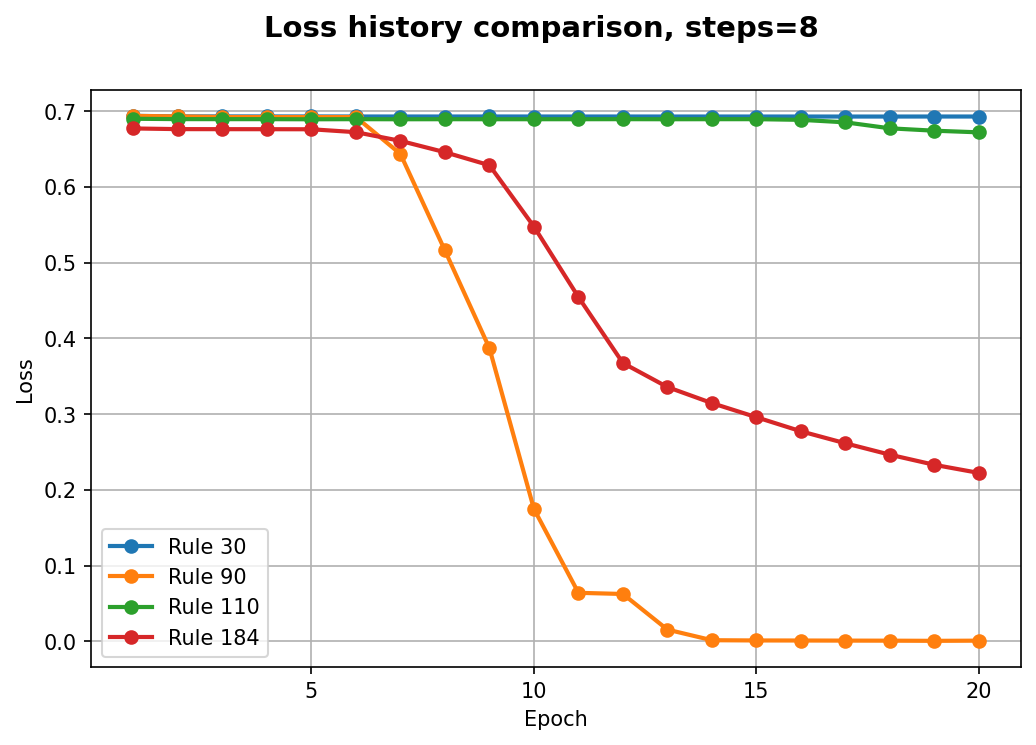
\includegraphics[height=10em]{../results/generalize_steps_8/loss_history_comparison.png}
    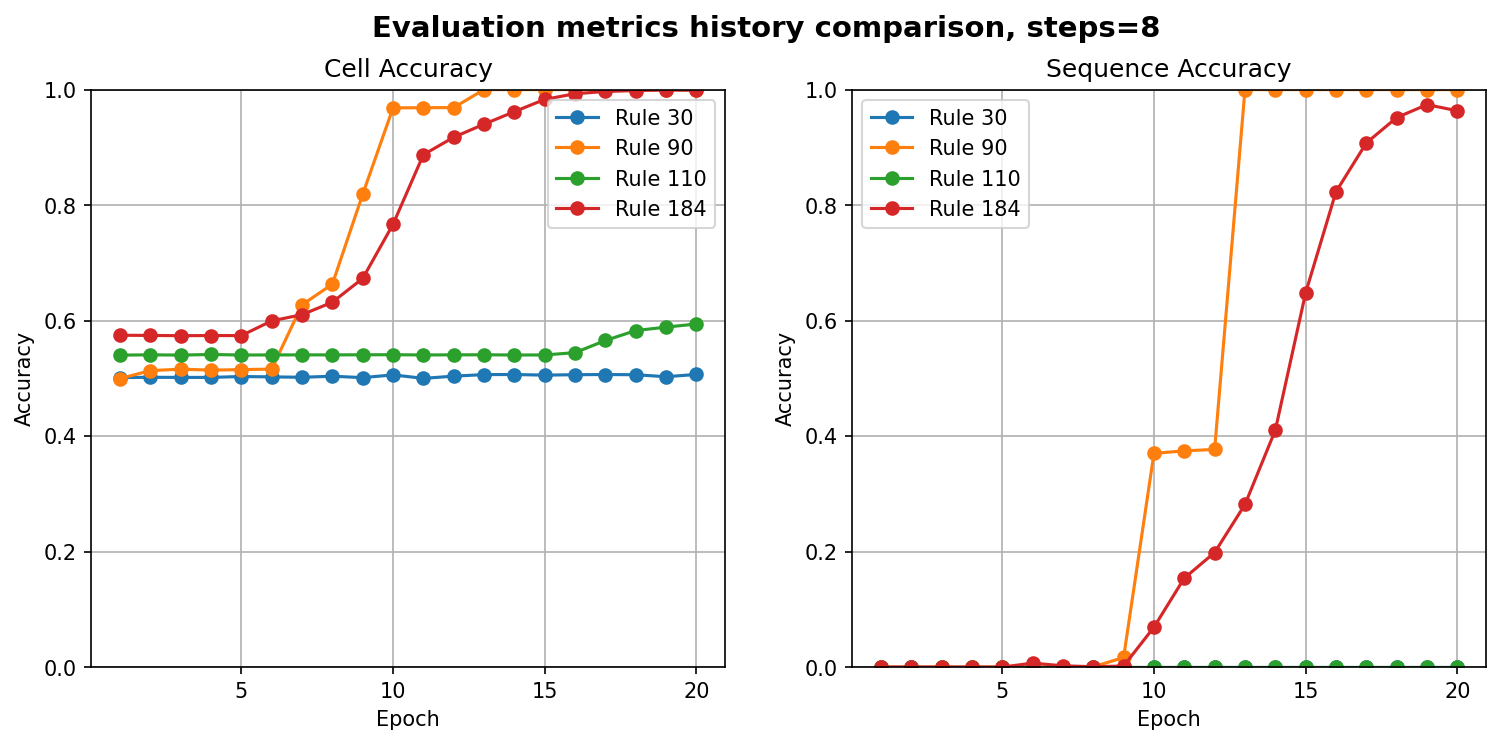
\includegraphics[height=10em]{../results/generalize_steps_8/eval_history_comparison.png}\\
    \caption{Training loss and evaluation metrics history for different number of steps prediction: from top to bottom, $k = 5, 6, 7, 8$.}
    \label{fig:loss-history-multi-step-2}
\end{figure}

\begin{figure}[ht]
    \centering
        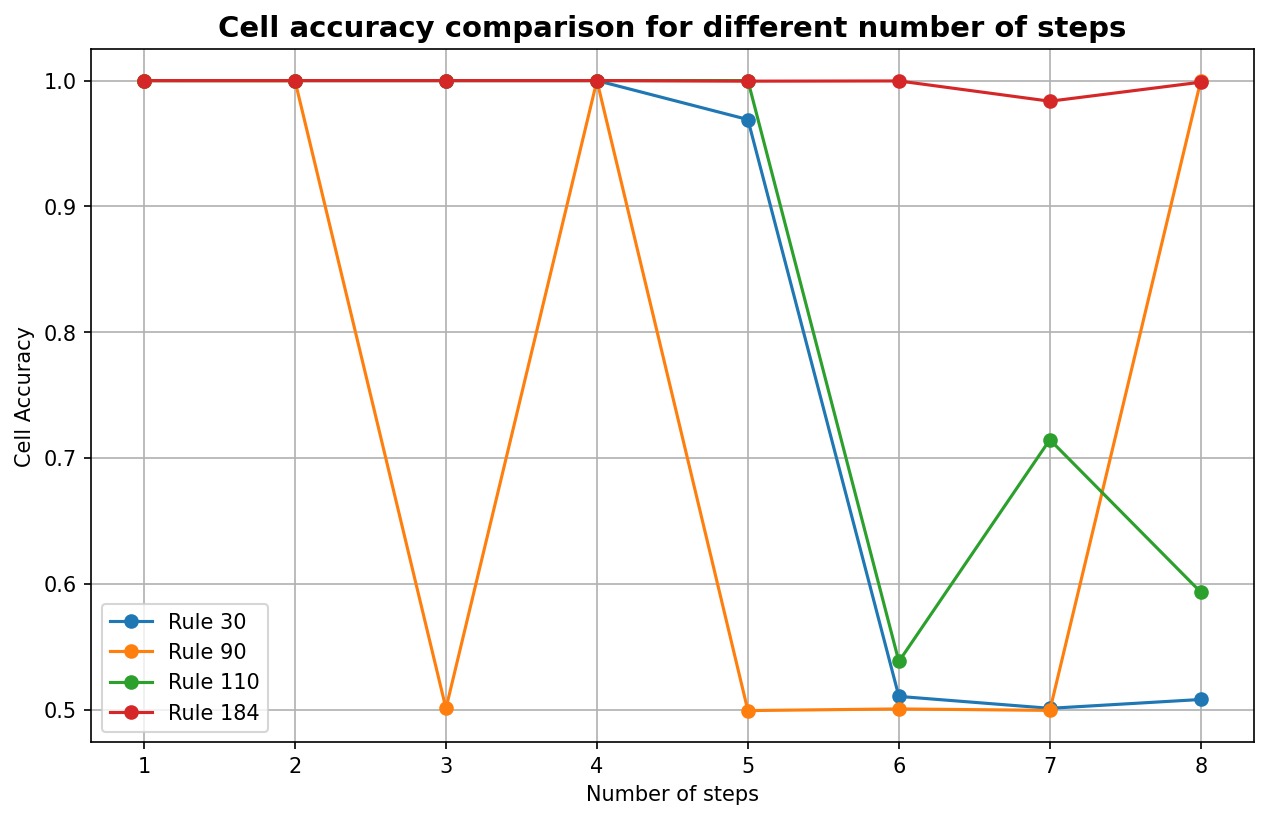
\includegraphics[width=\linewidth]{../results/generalize_steps/cell_accuracy_comparison.png}
        \caption{Cell accuracy evaluated for different number of steps prediction.}
    \label{fig:cell-accuracy-multi-step}
\end{figure}

We also analyzed the attention maps, which are shown in \cref{fig:attention-multi-step} (we averaged the weights across all layers and heads). We can see that for small values of $k$ all rules show the diagonal pattern, which is also becoming wider as $k$ increases. This is expected since the model needs to attend to a wider neighborhood to predict further time steps. For larger values of $k$, some rules show a ``global'' attention pattern.

The ``nicest'' patterns are shown by Rule 184, which are becoming wider one cell each time number of prediction steps increases. We can also see an interesting pattern for Rule 90 and $k = 4$ and $k = 8$ -- the pattern is not a single diagonal as usual, but two distinct diagonals together with some diffuse attention in between. This supports the hypothesis that the states after $2^n$ steps contain some kind of regularity and structure that the model can learn. After all, Rule 90 is based on XOR operation, which certainly has some kinf od regularity and structure.

\begin{itemize}
    \item \textbf{Rule 30} --
\end{itemize}

\begin{figure}[ht]
    \centering
    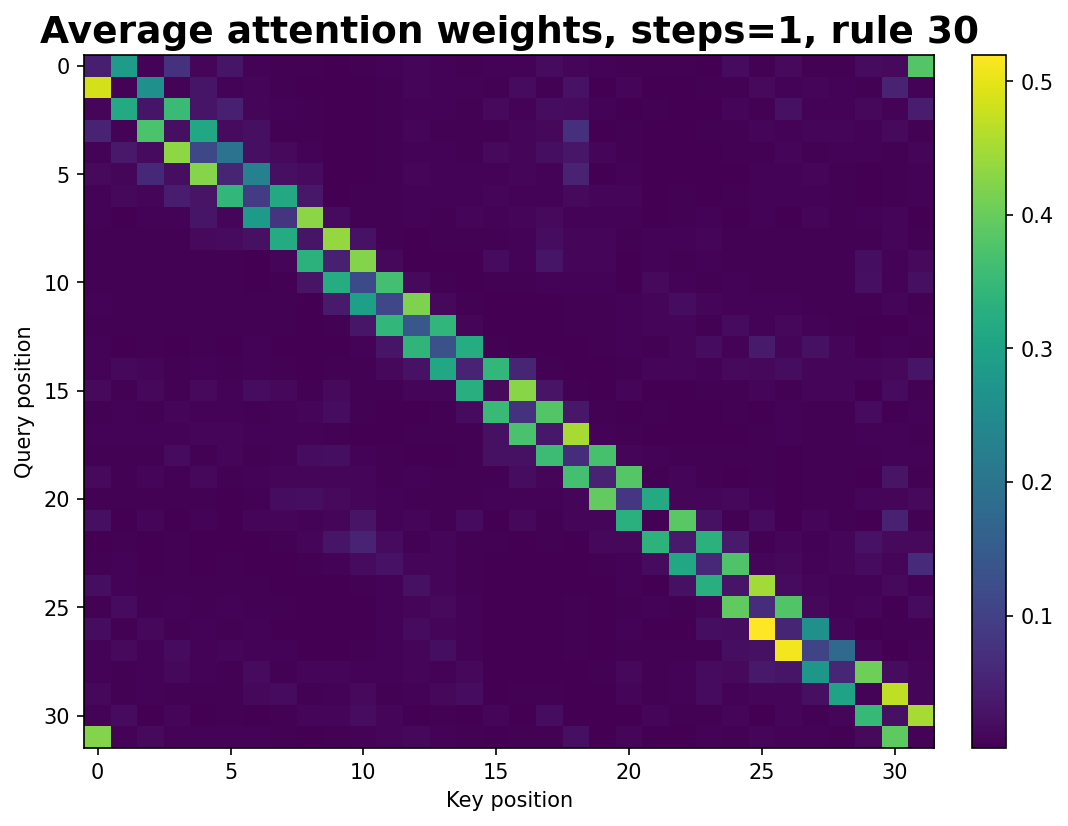
\includegraphics[width=0.23\linewidth]{../results/generalize_steps_1/average_attention_rule_30.png}
    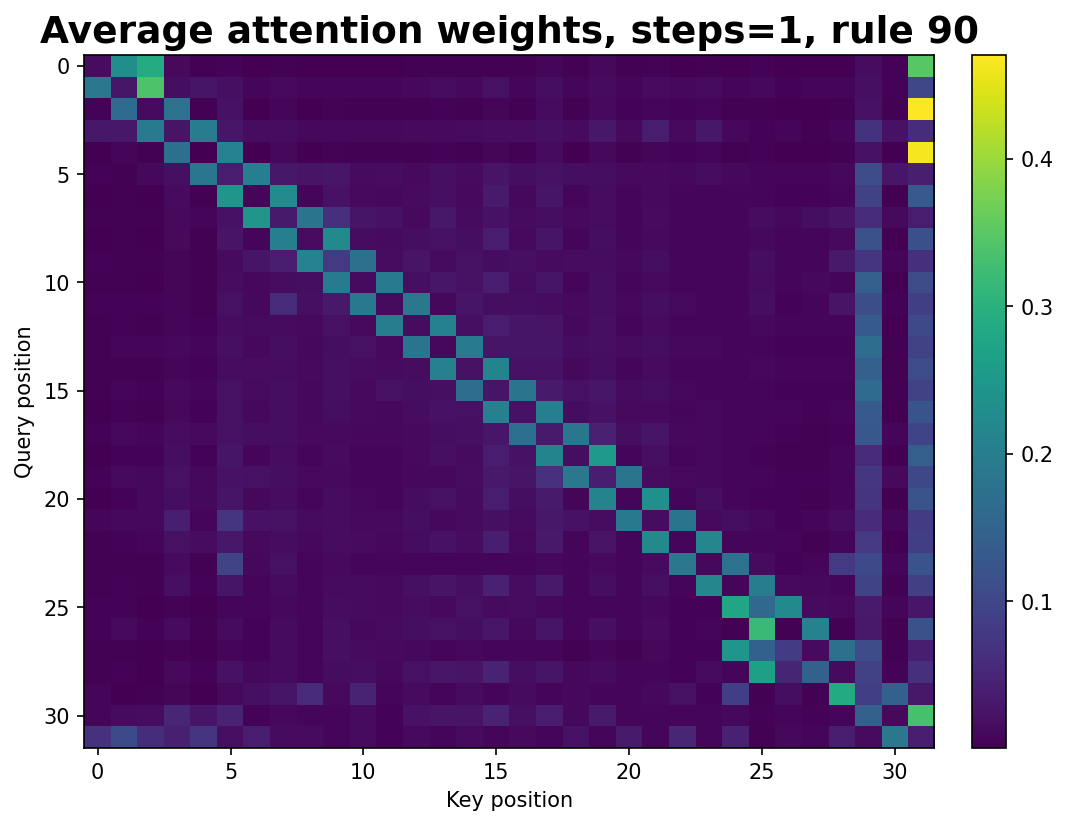
\includegraphics[width=0.23\linewidth]{../results/generalize_steps_1/average_attention_rule_90.png}
    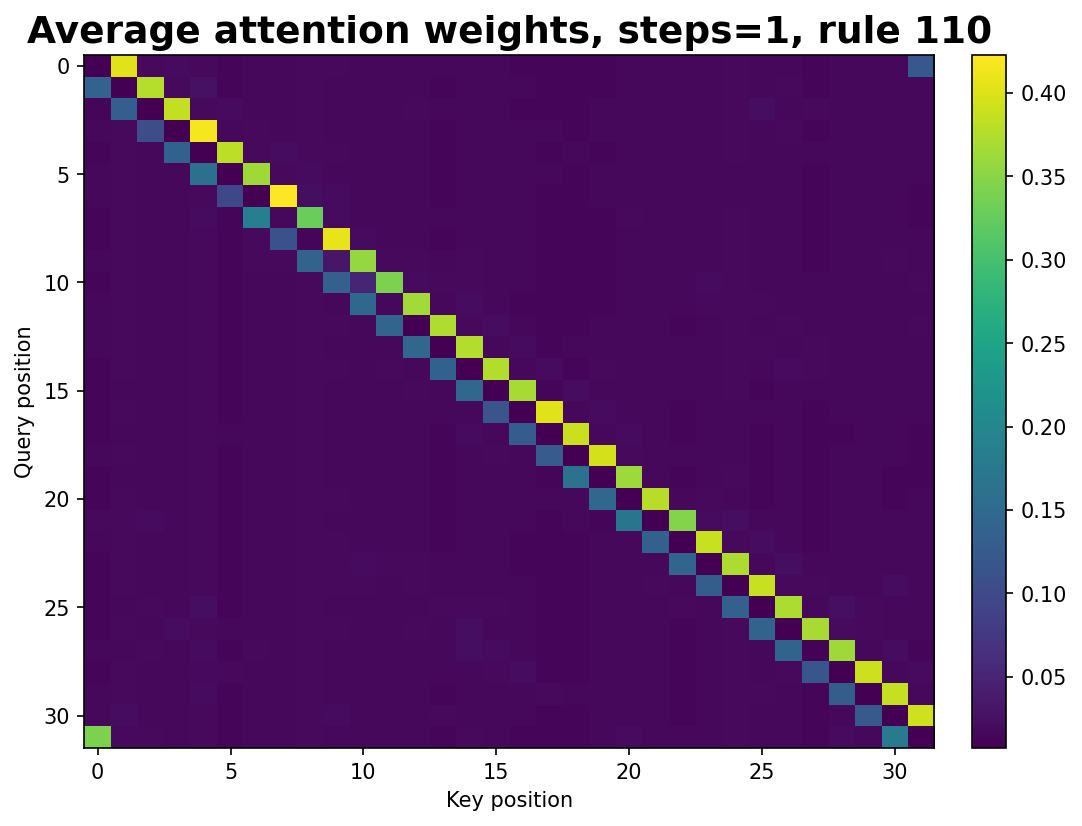
\includegraphics[width=0.23\linewidth]{../results/generalize_steps_1/average_attention_rule_110.png}
    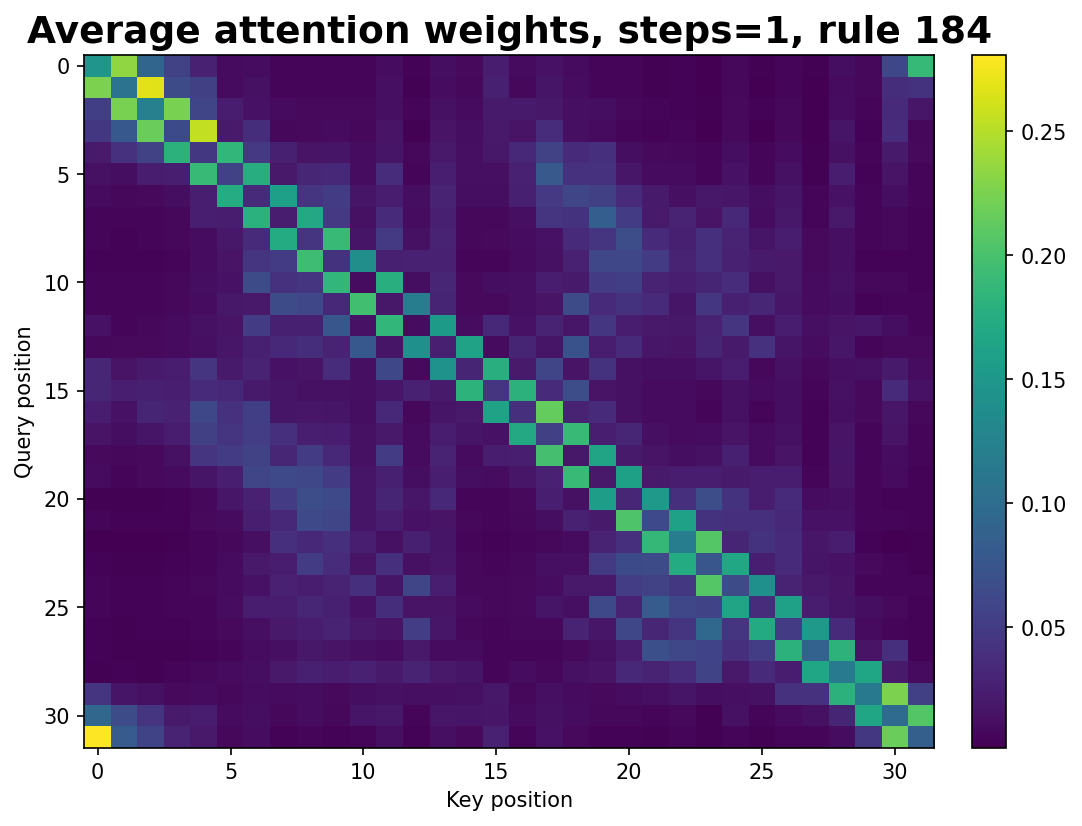
\includegraphics[width=0.23\linewidth]{../results/generalize_steps_1/average_attention_rule_184.png}\\
    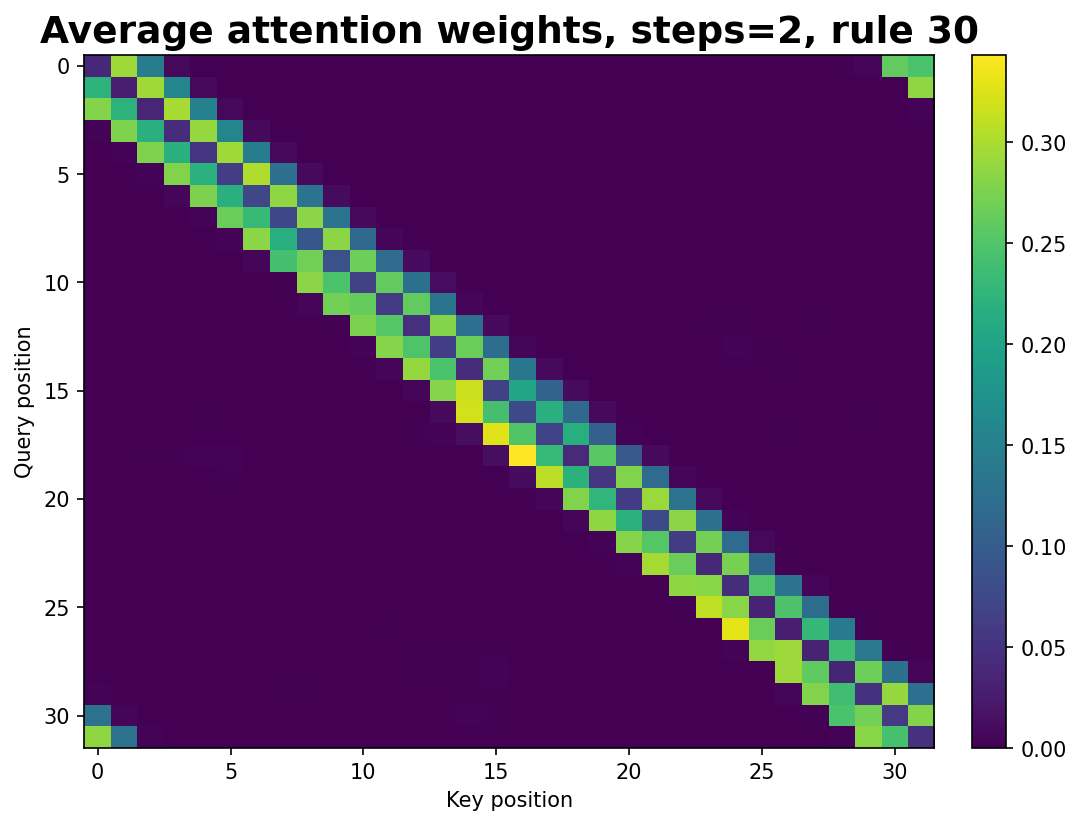
\includegraphics[width=0.23\linewidth]{../results/generalize_steps_2/average_attention_rule_30.png}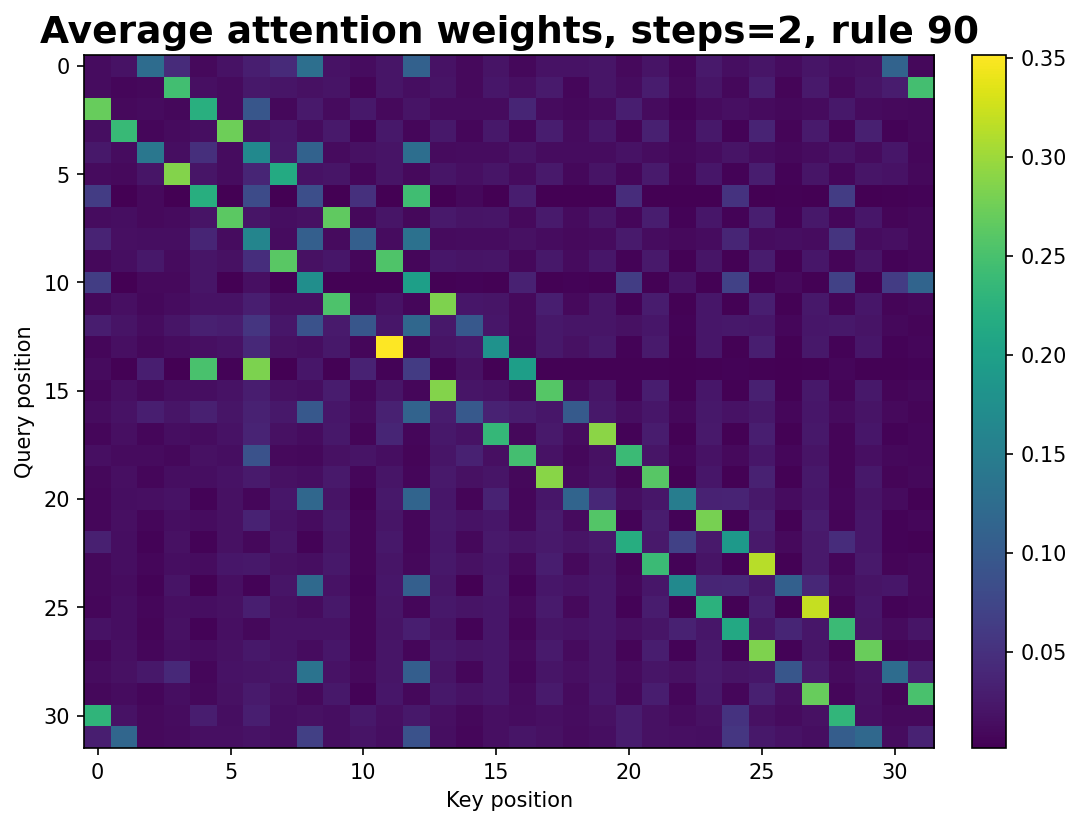
\includegraphics[width=0.23\linewidth]{../results/generalize_steps_2/average_attention_rule_90.png}
    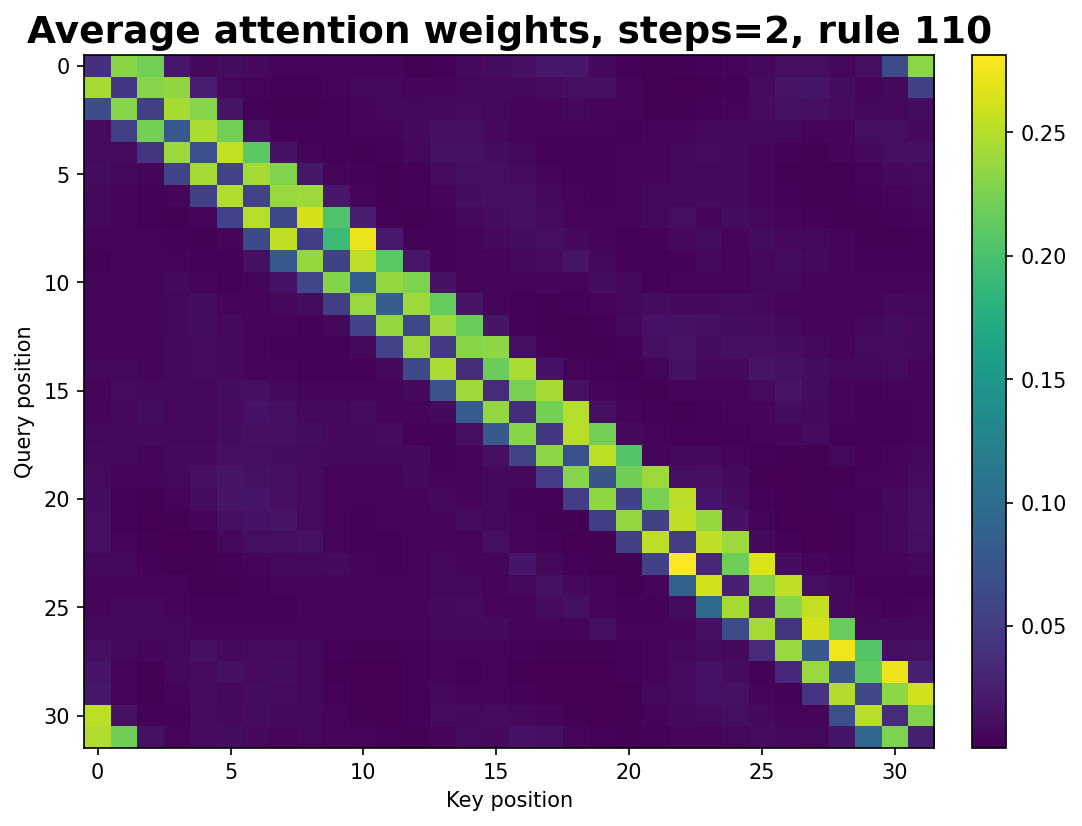
\includegraphics[width=0.23\linewidth]{../results/generalize_steps_2/average_attention_rule_110.png}
    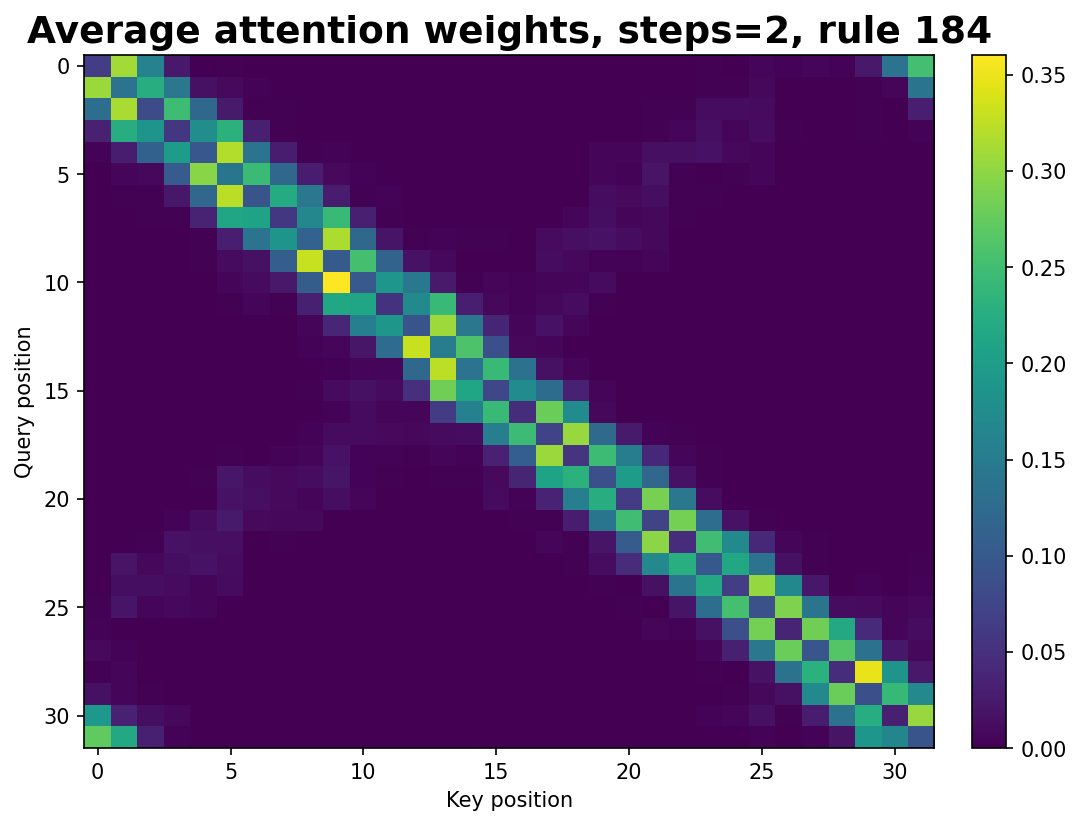
\includegraphics[width=0.23\linewidth]{../results/generalize_steps_2/average_attention_rule_184.png}\\
    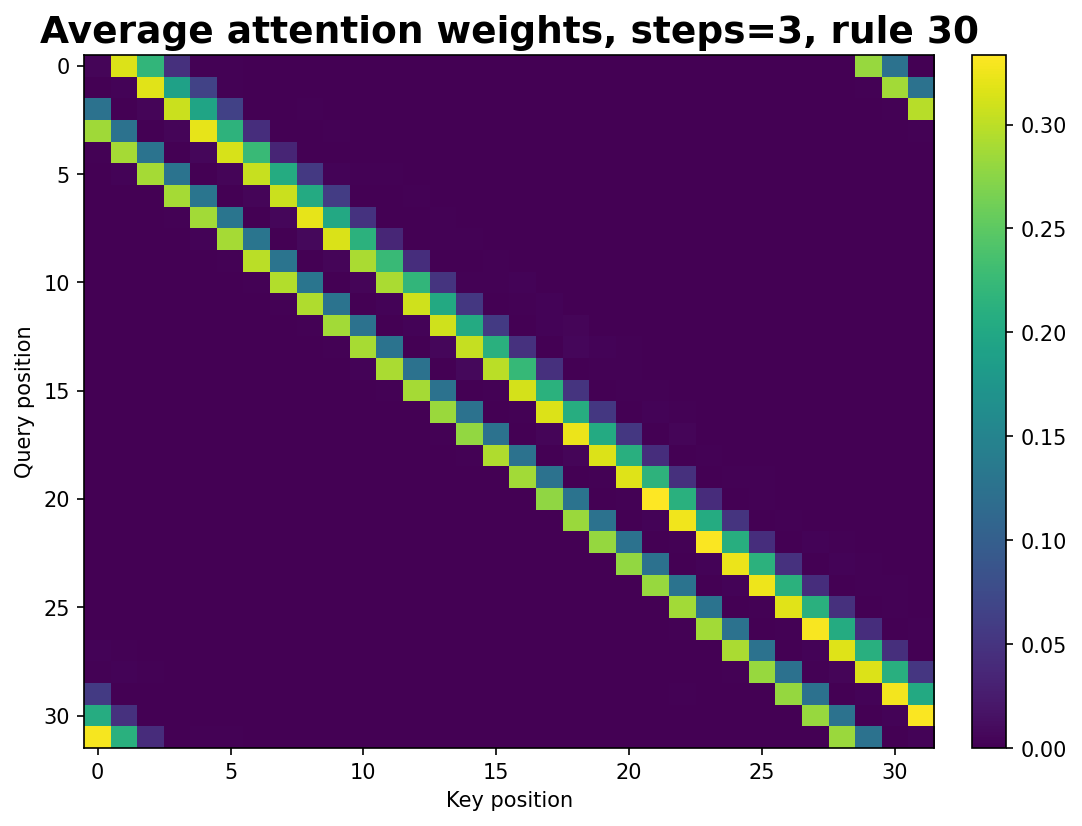
\includegraphics[width=0.23\linewidth]{../results/generalize_steps_3/average_attention_rule_30.png}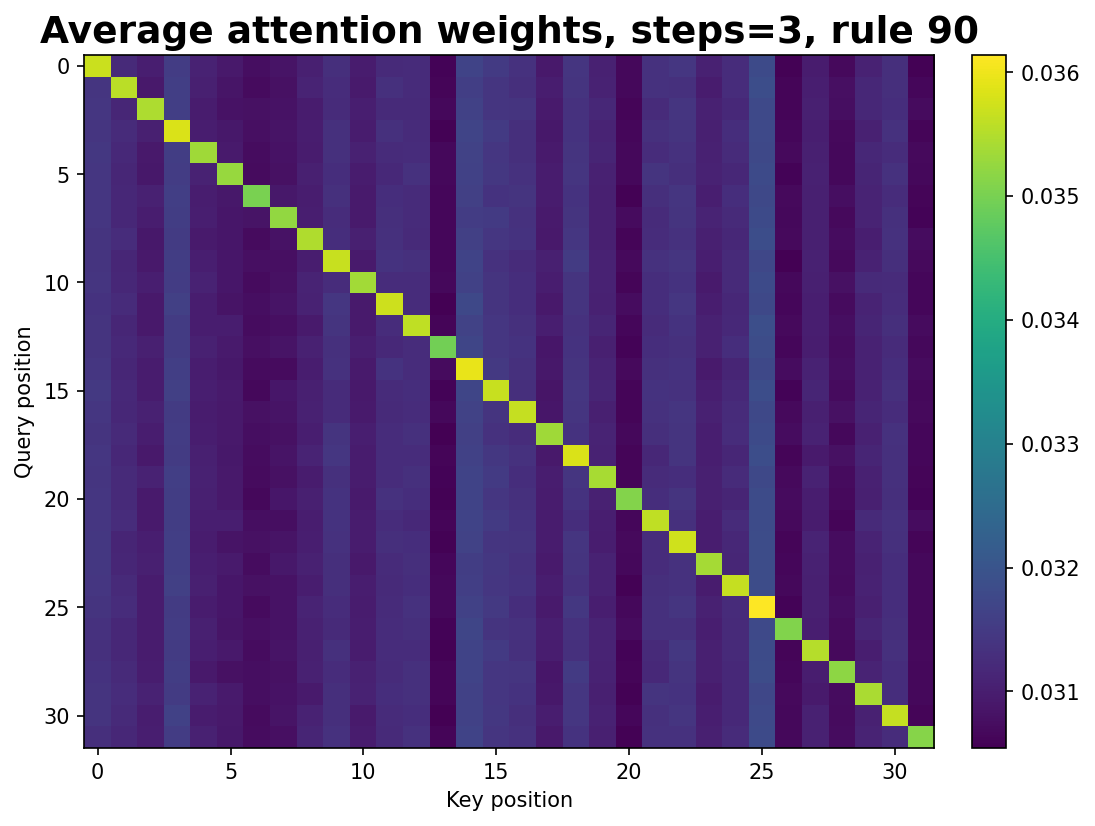
\includegraphics[width=0.23\linewidth]{../results/generalize_steps_3/average_attention_rule_90.png}
    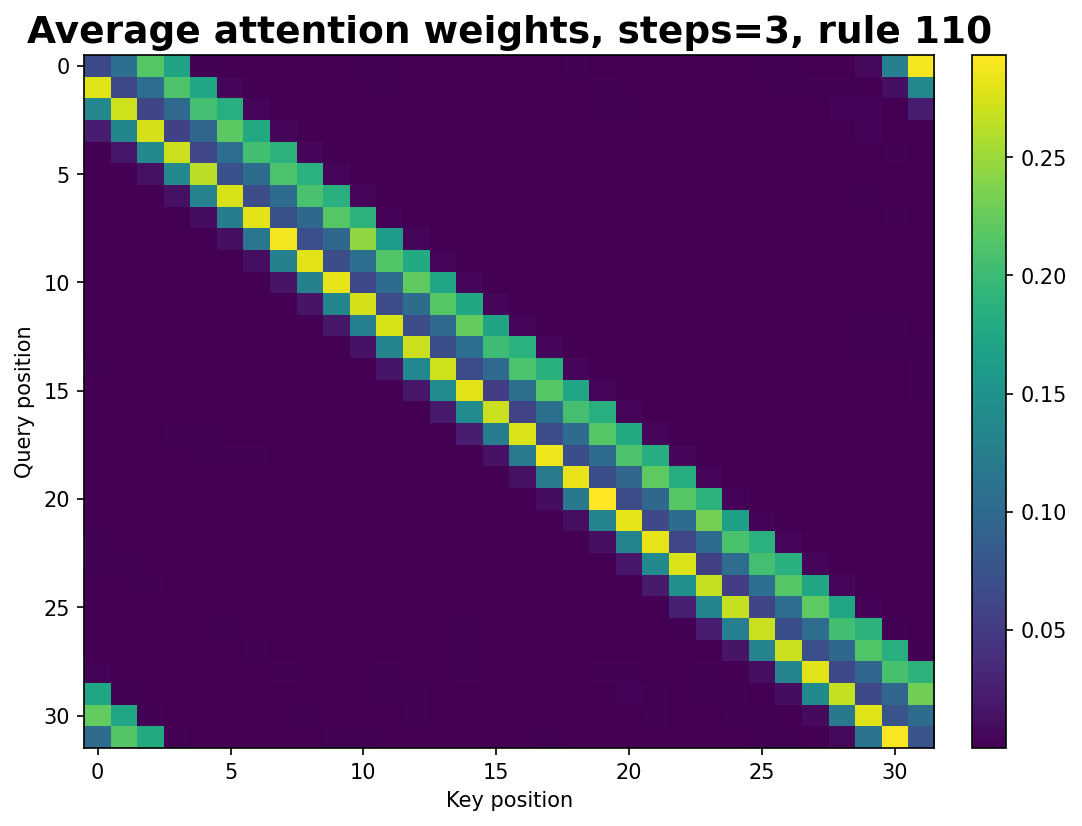
\includegraphics[width=0.23\linewidth]{../results/generalize_steps_3/average_attention_rule_110.png}
    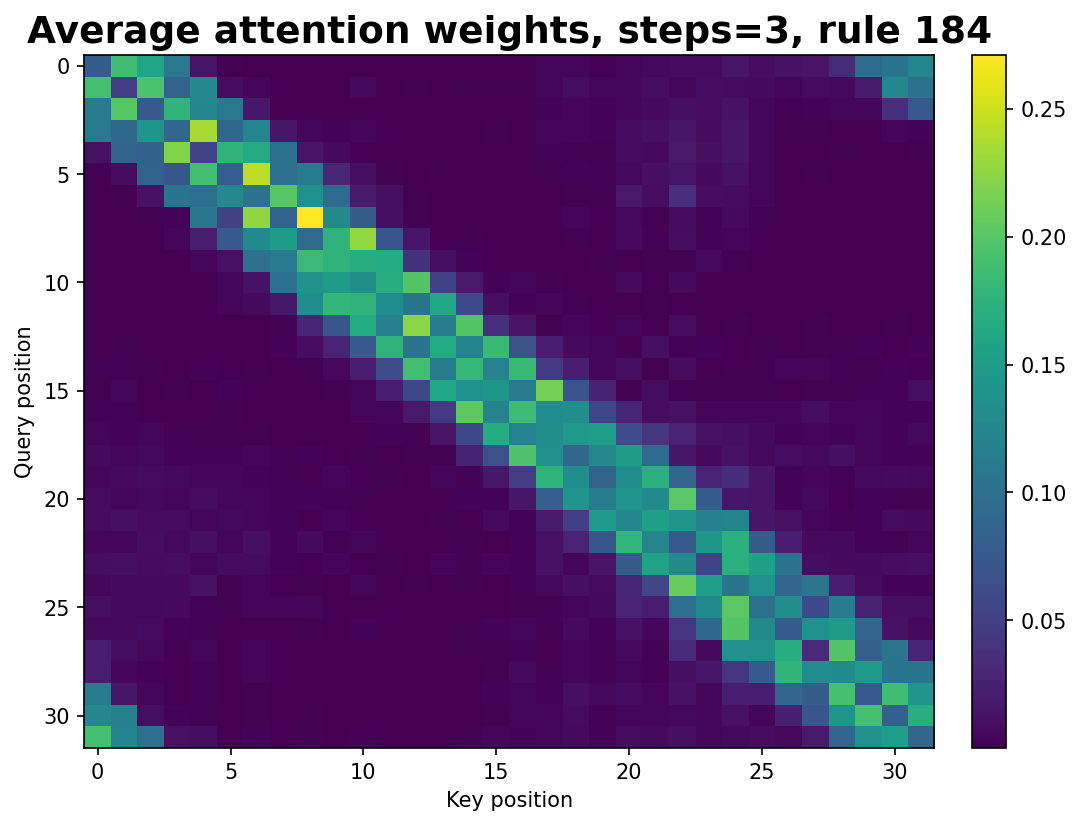
\includegraphics[width=0.23\linewidth]{../results/generalize_steps_3/average_attention_rule_184.png}\\
    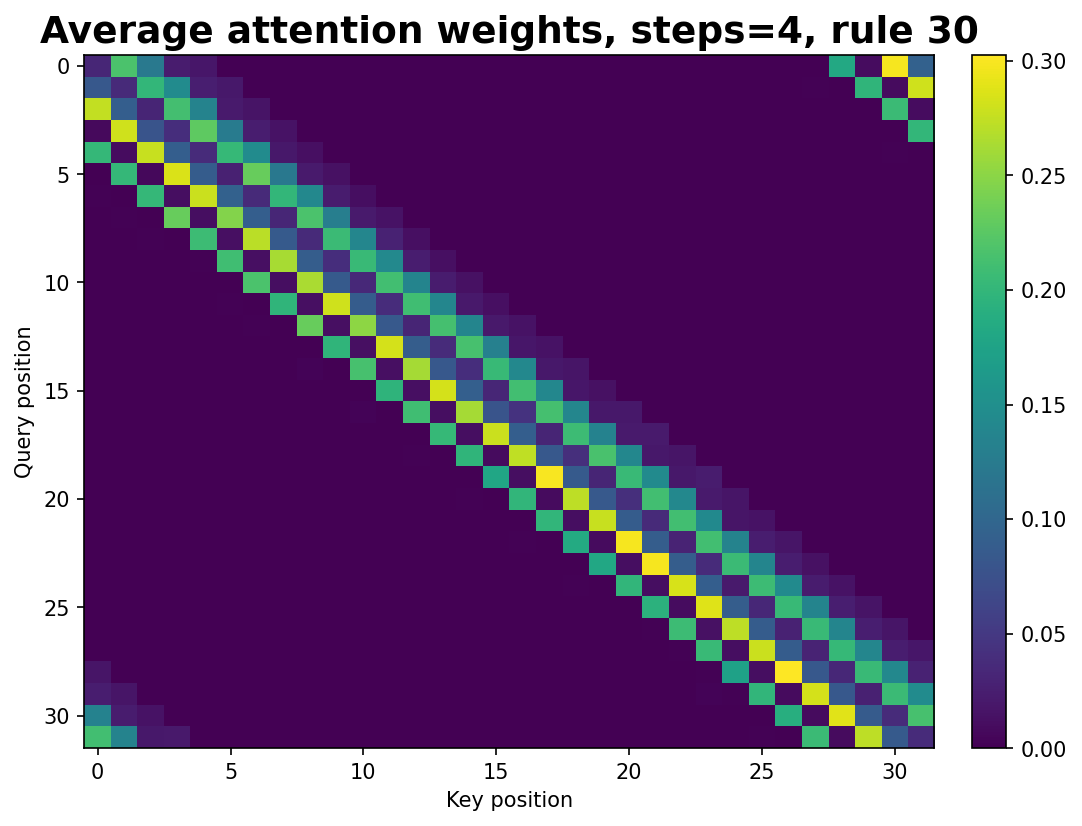
\includegraphics[width=0.23\linewidth]{../results/generalize_steps_4/average_attention_rule_30.png}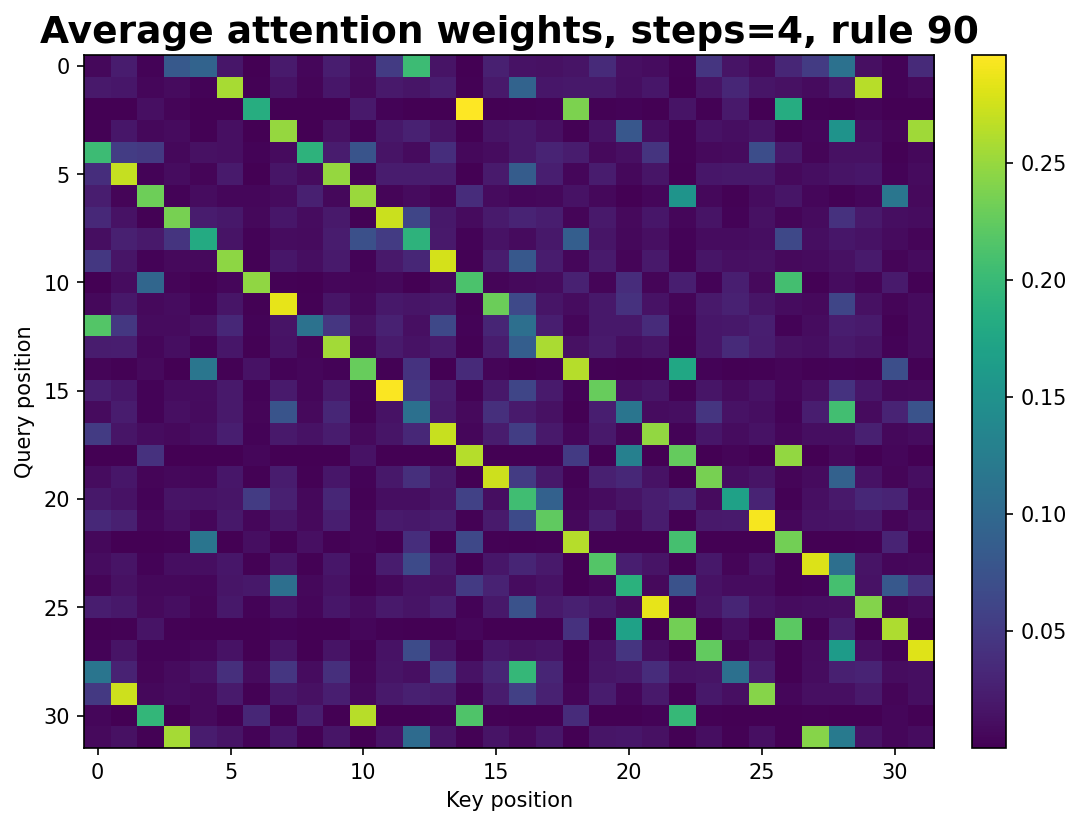
\includegraphics[width=0.23\linewidth]{../results/generalize_steps_4/average_attention_rule_90.png}
    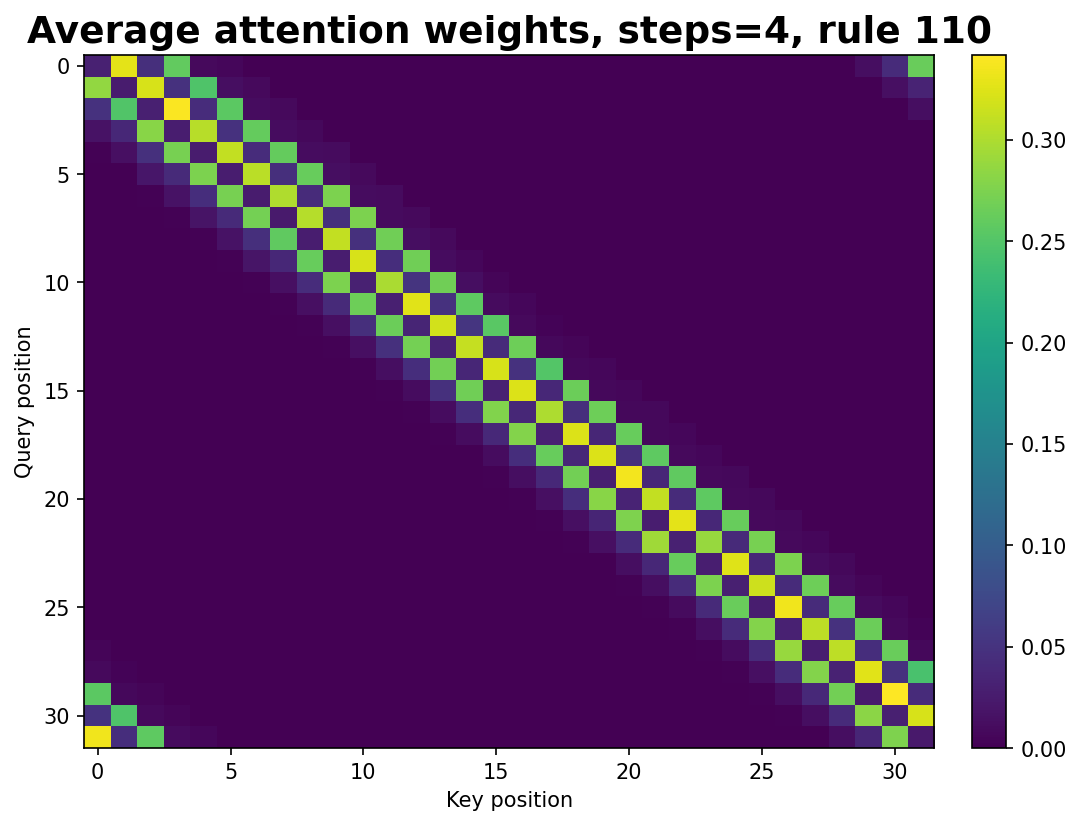
\includegraphics[width=0.23\linewidth]{../results/generalize_steps_4/average_attention_rule_110.png}
    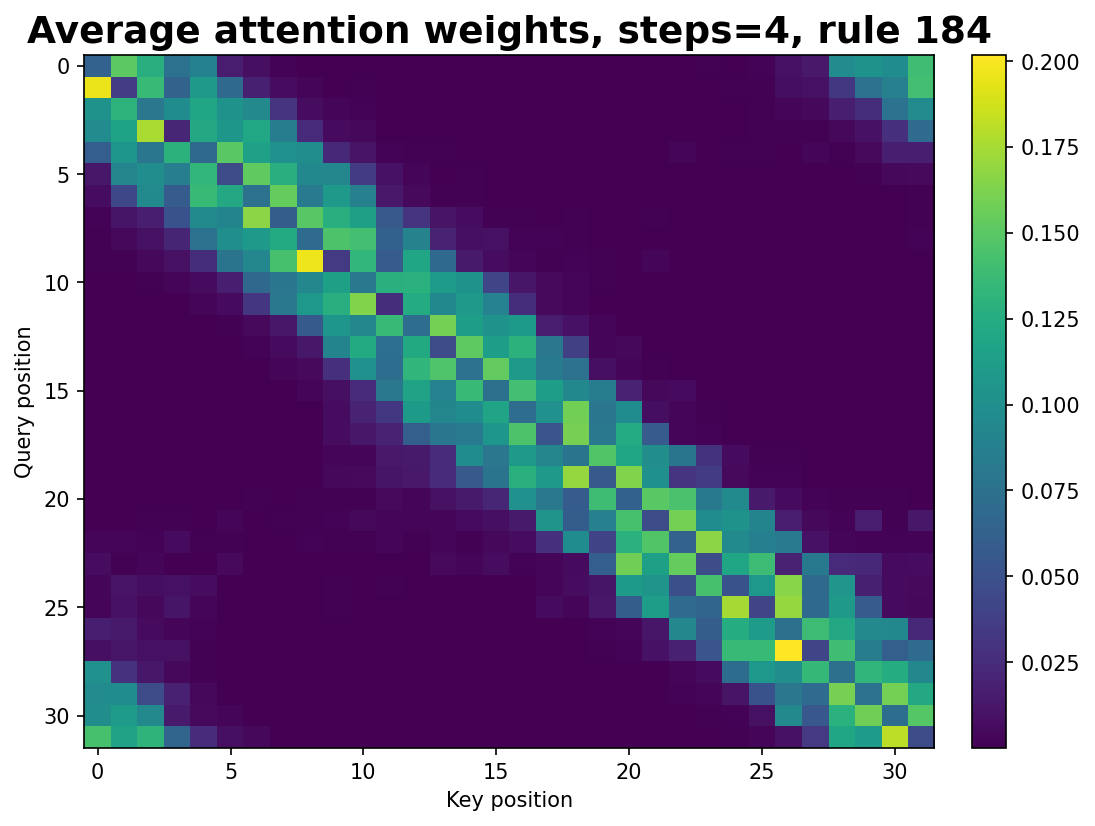
\includegraphics[width=0.23\linewidth]{../results/generalize_steps_4/average_attention_rule_184.png}\\
    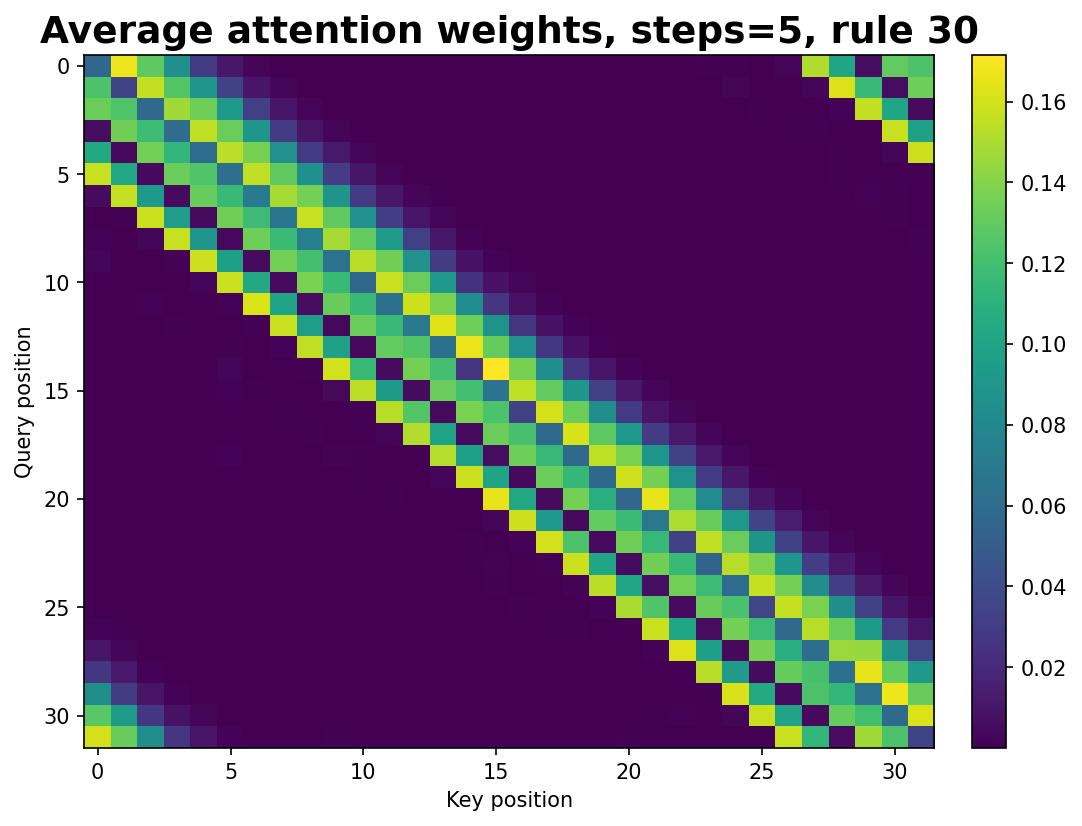
\includegraphics[width=0.23\linewidth]{../results/generalize_steps_5/average_attention_rule_30.png}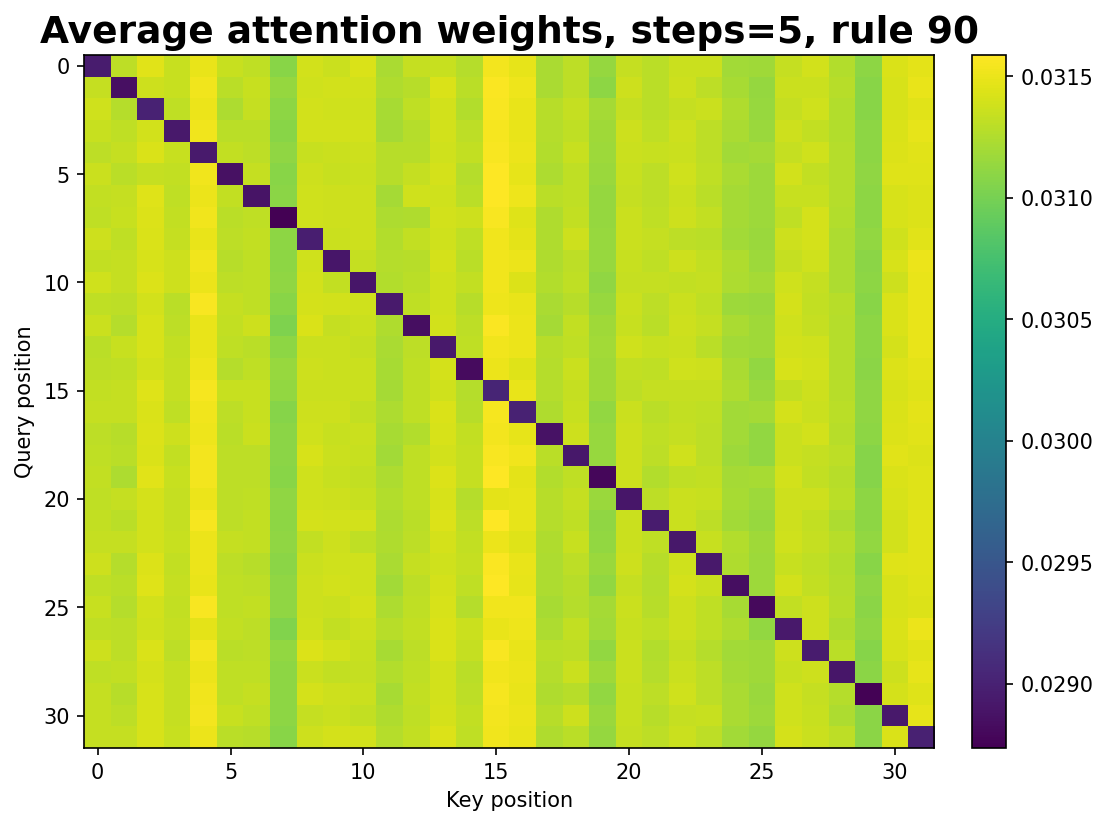
\includegraphics[width=0.23\linewidth]{../results/generalize_steps_5/average_attention_rule_90.png}
    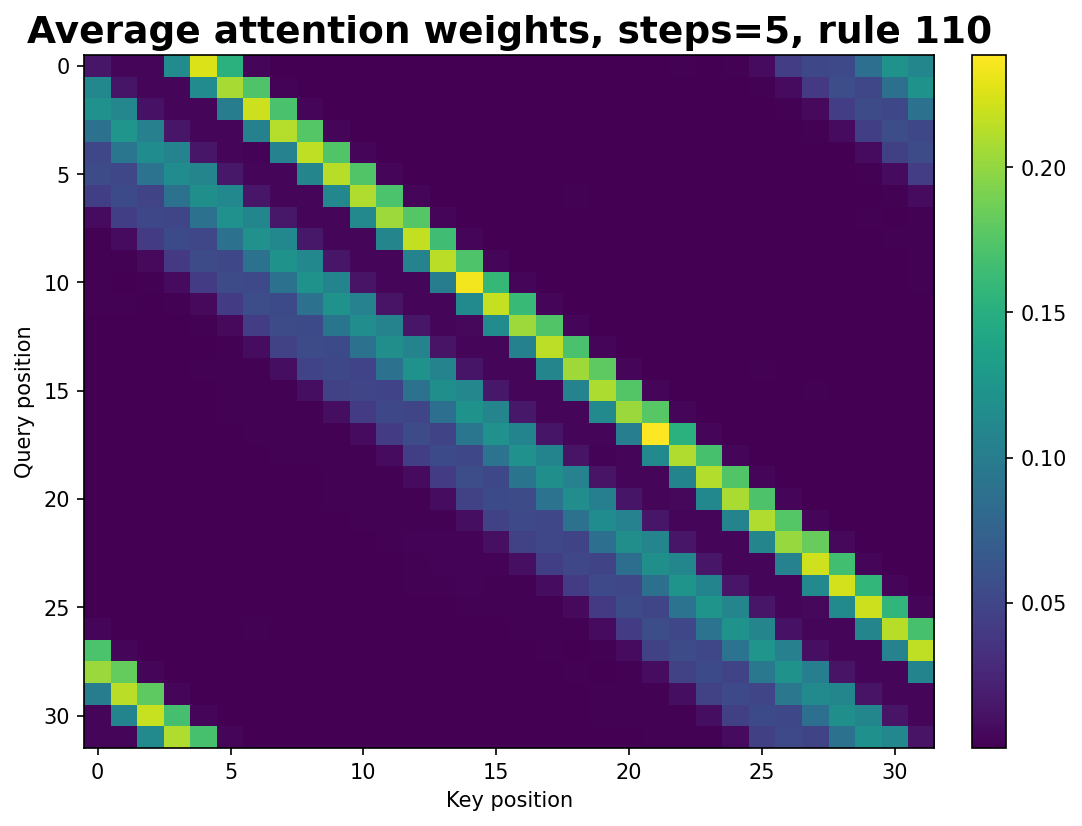
\includegraphics[width=0.23\linewidth]{../results/generalize_steps_5/average_attention_rule_110.png}
    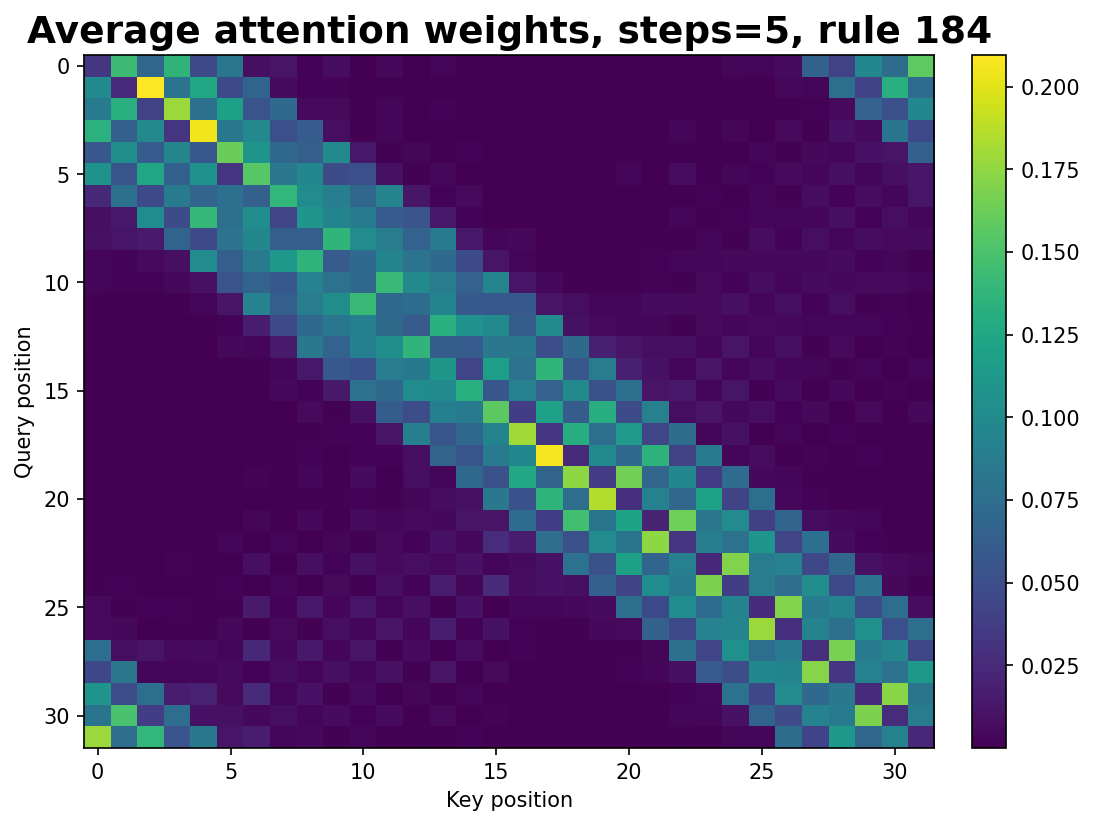
\includegraphics[width=0.23\linewidth]{../results/generalize_steps_5/average_attention_rule_184.png}\\
    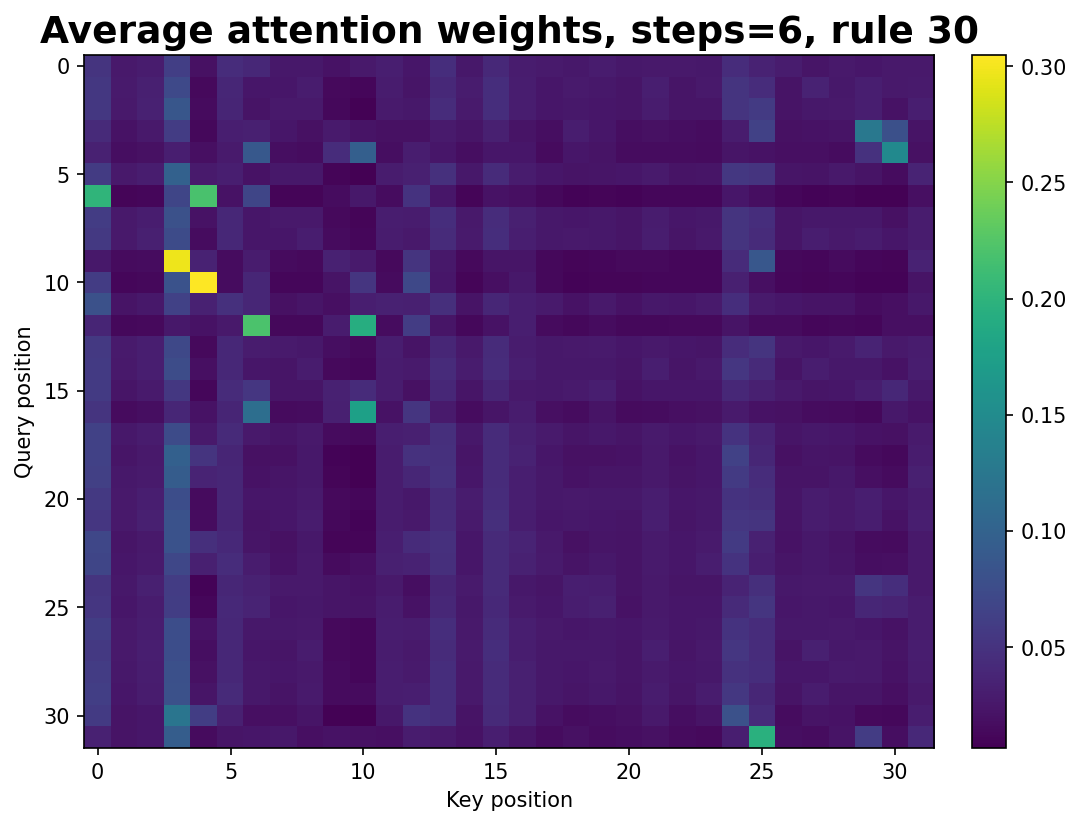
\includegraphics[width=0.23\linewidth]{../results/generalize_steps_6/average_attention_rule_30.png}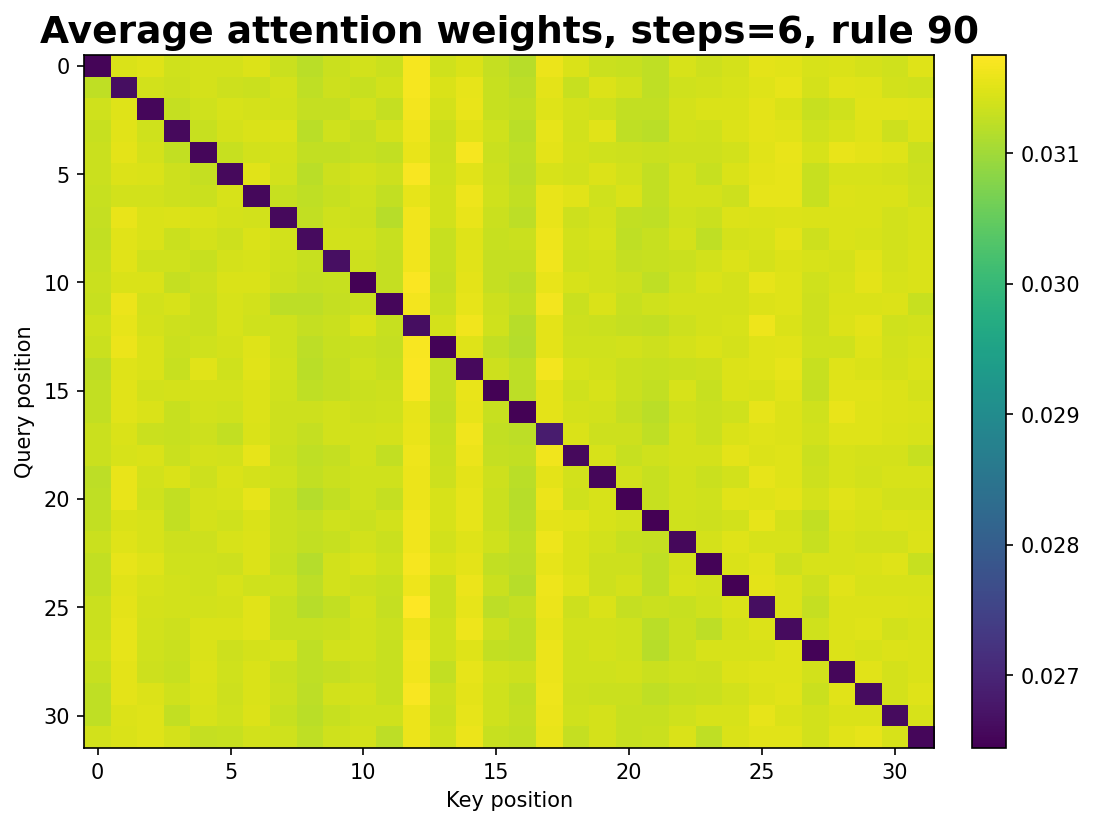
\includegraphics[width=0.23\linewidth]{../results/generalize_steps_6/average_attention_rule_90.png}
    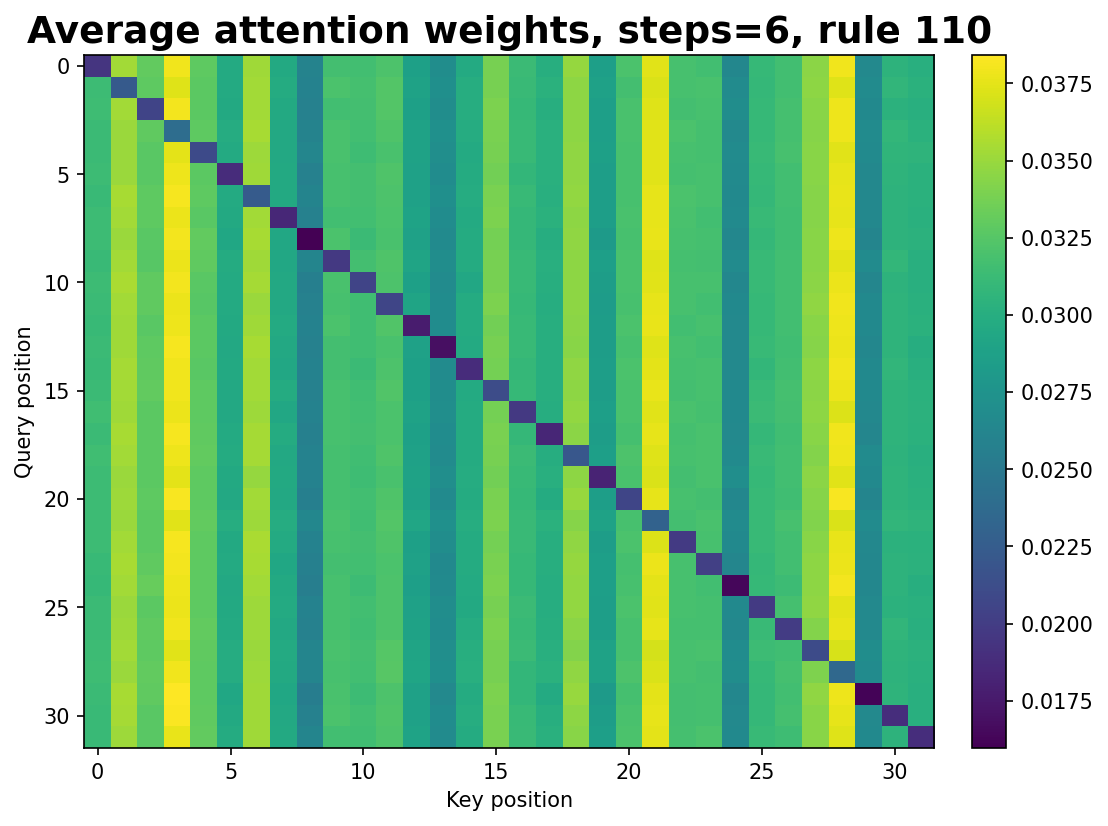
\includegraphics[width=0.23\linewidth]{../results/generalize_steps_6/average_attention_rule_110.png}
    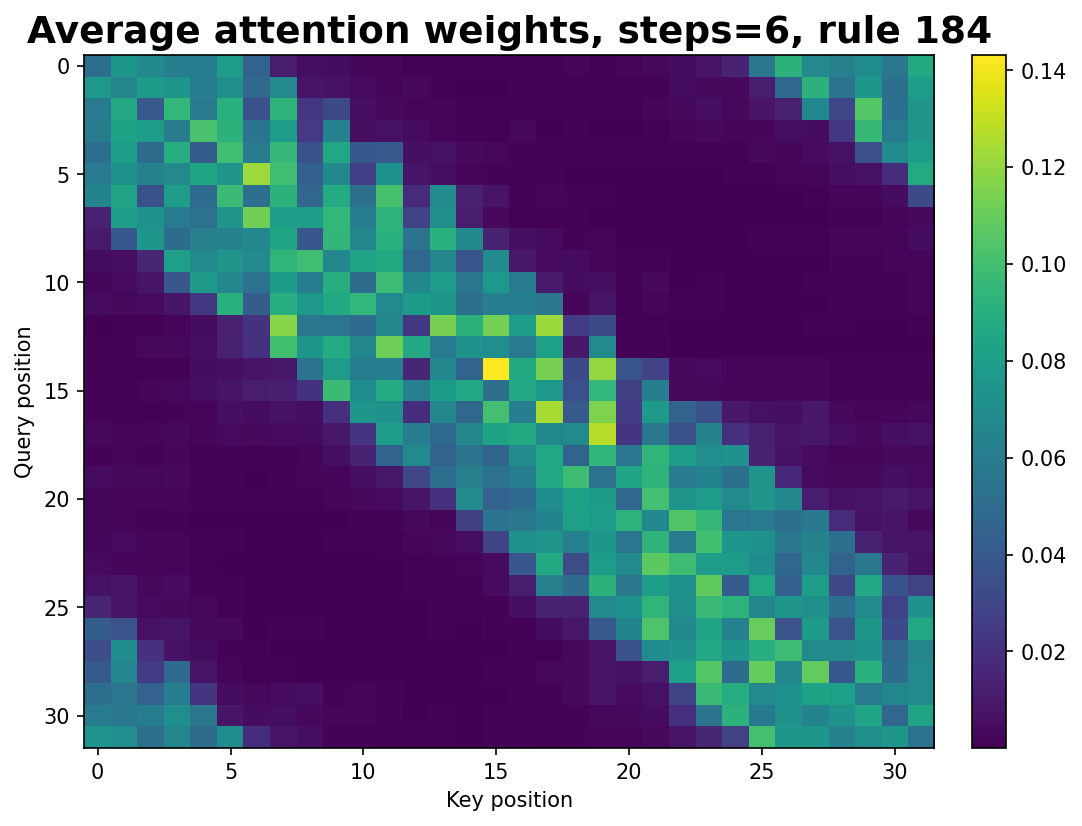
\includegraphics[width=0.23\linewidth]{../results/generalize_steps_6/average_attention_rule_184.png}\\
    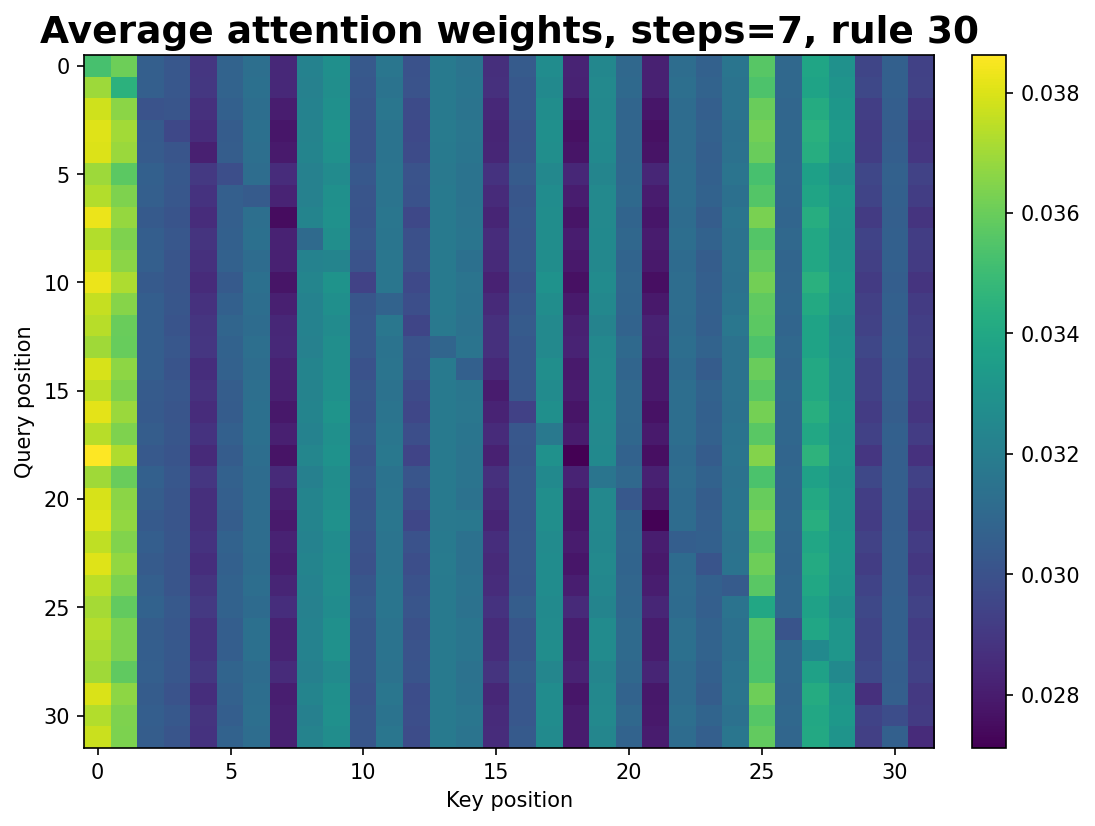
\includegraphics[width=0.23\linewidth]{../results/generalize_steps_7/average_attention_rule_30.png}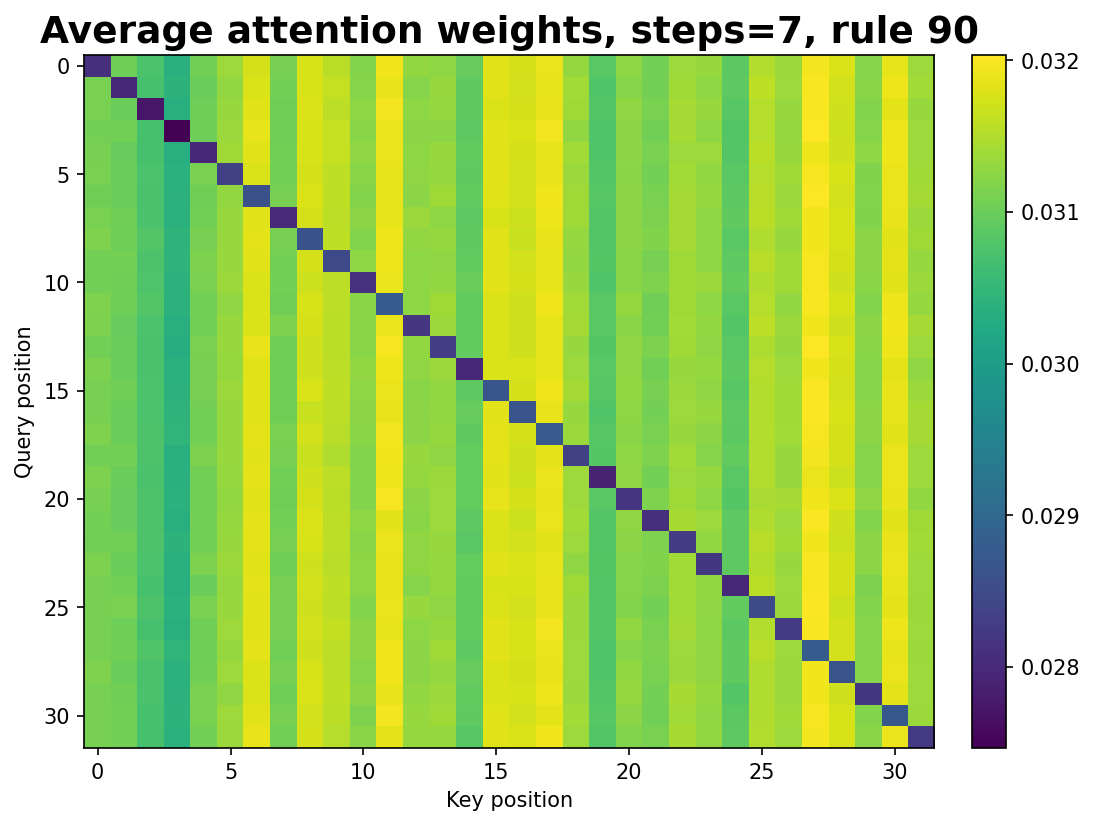
\includegraphics[width=0.23\linewidth]{../results/generalize_steps_7/average_attention_rule_90.png}
    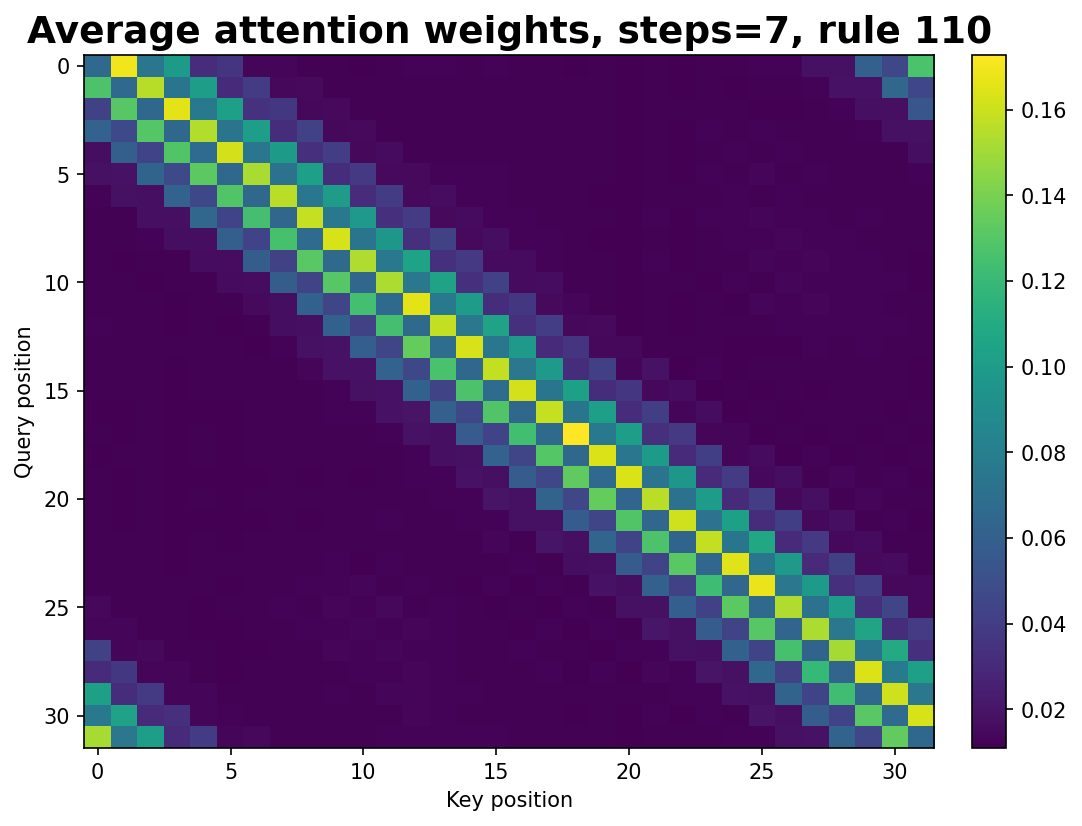
\includegraphics[width=0.23\linewidth]{../results/generalize_steps_7/average_attention_rule_110.png}
    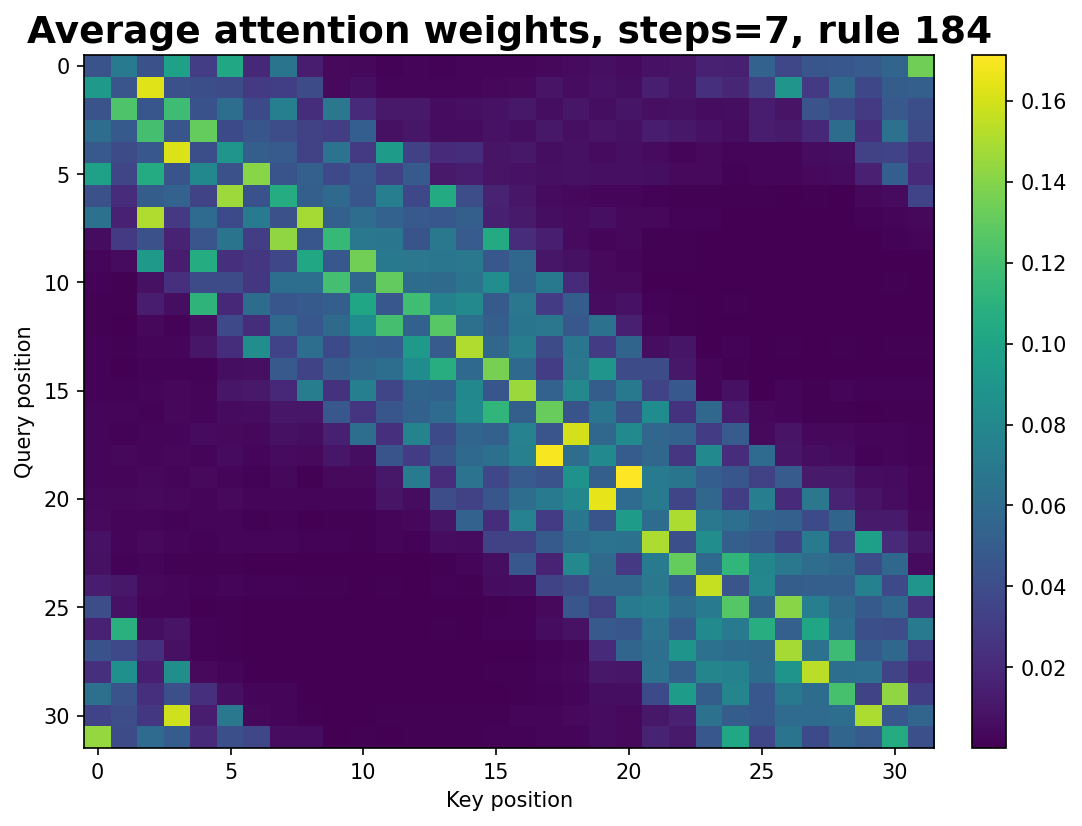
\includegraphics[width=0.23\linewidth]{../results/generalize_steps_7/average_attention_rule_184.png}\\
    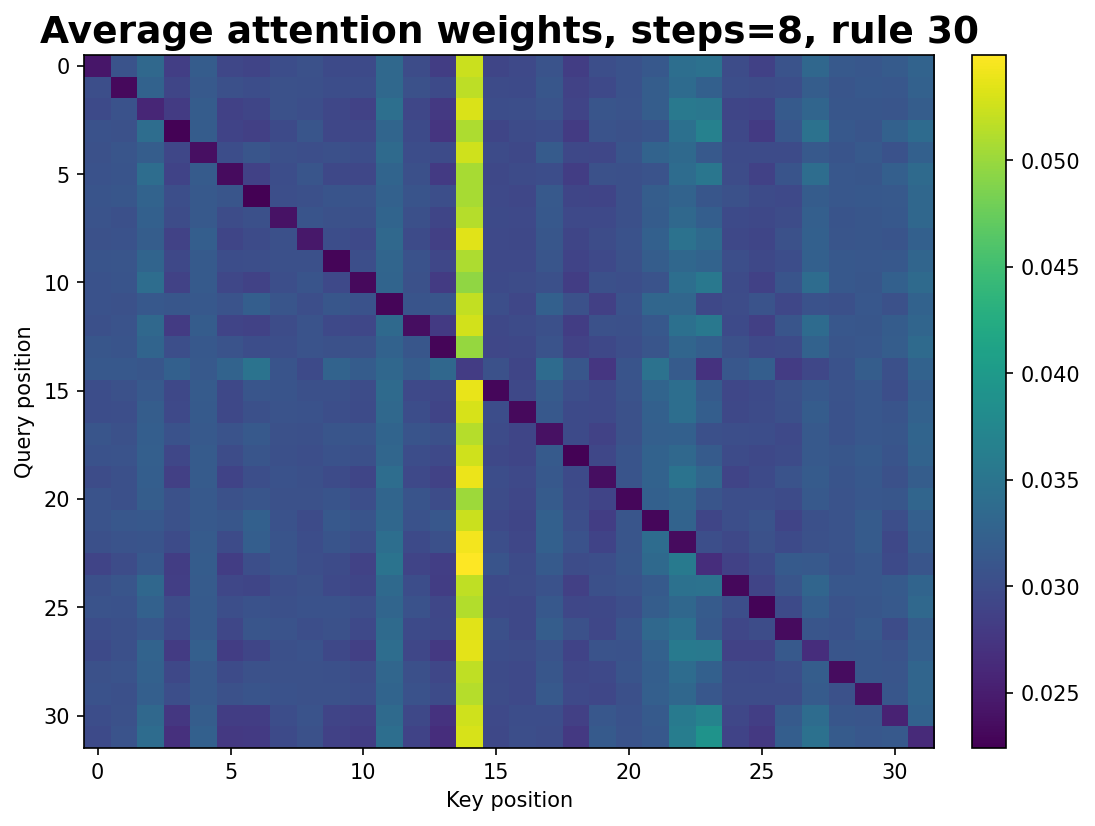
\includegraphics[width=0.23\linewidth]{../results/generalize_steps_8/average_attention_rule_30.png}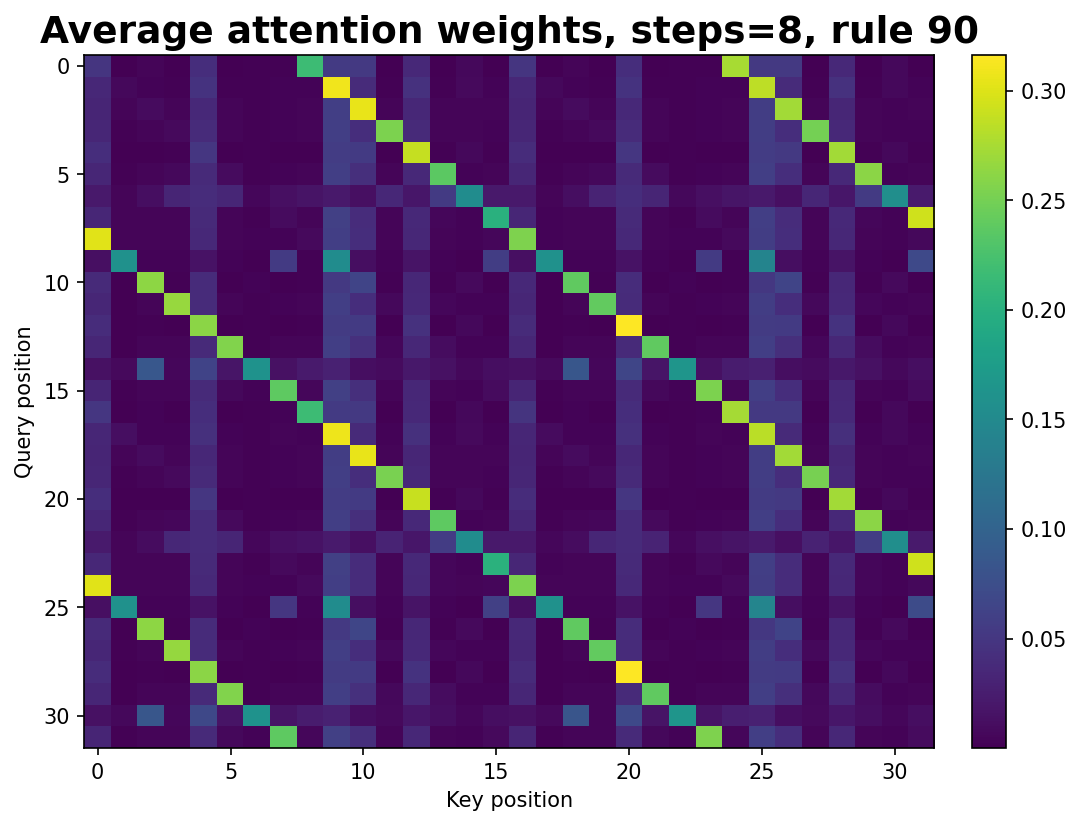
\includegraphics[width=0.23\linewidth]{../results/generalize_steps_8/average_attention_rule_90.png}
    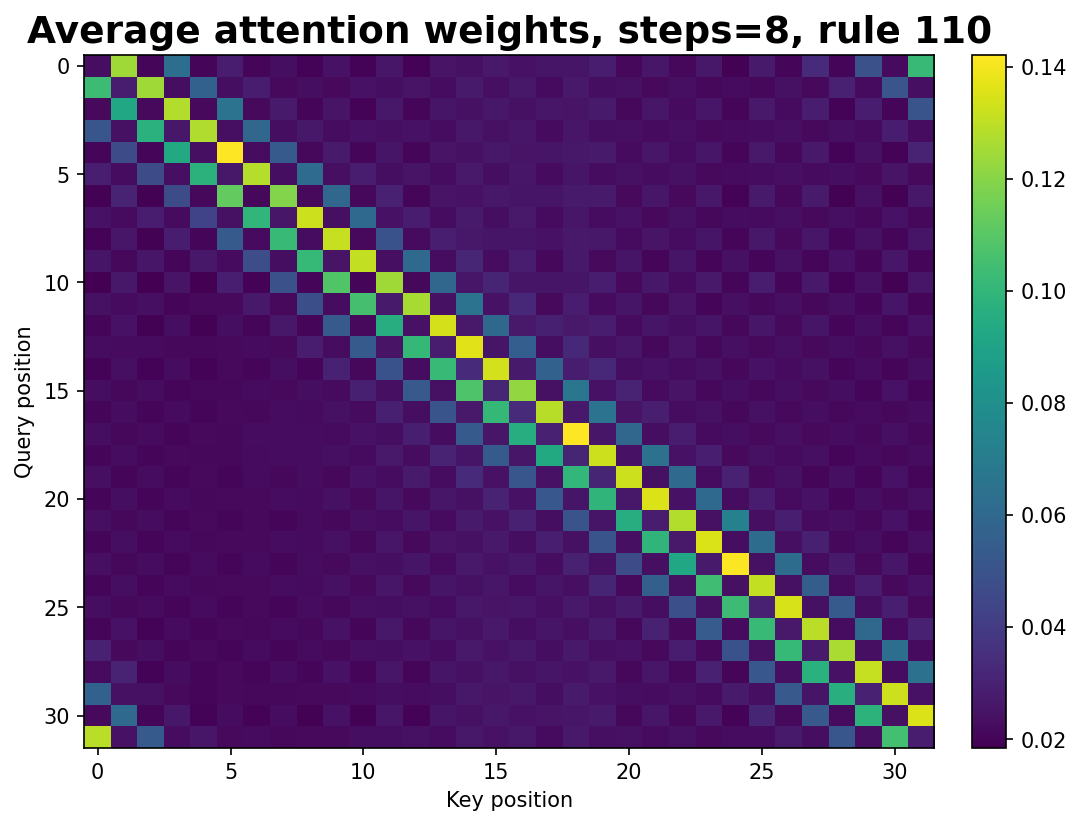
\includegraphics[width=0.23\linewidth]{../results/generalize_steps_8/average_attention_rule_110.png}
    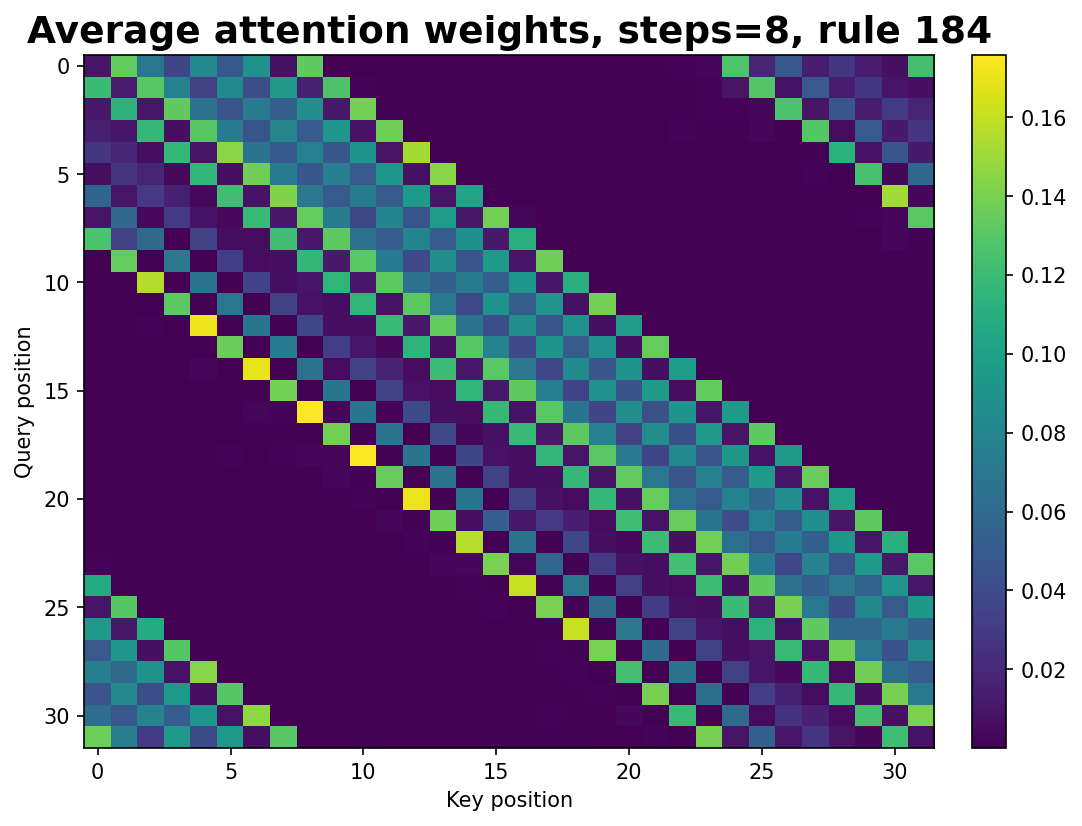
\includegraphics[width=0.23\linewidth]{../results/generalize_steps_8/average_attention_rule_184.png}\\
    \caption{Average attention weights for different number of steps prediction: from top to bottom, $k = 1, 2, \dots, 8$, from left to right, Rule 30, Rule 90, Rule 110, Rule 184. Each image shows the average attention weights across all layers and heads and across all test samples.}
    \label{fig:average-attention-multi-step}
\end{figure}


\section{Other Generalization Experiments}
\label{sec:other-gen}

Although we did not have time to perform other generalization experiments, we would like to mention two other interesting directions for future work:

\begin{itemize}      
    \item \textbf{Generalization to different initial conditions} -- We could evaluate the model's performance on initial states that are significantly different from those seen during training, e.g., dense vectors vs. sparse vectors, or initial states with specific patterns.
    
    \item \textbf{Generalization to different rules} -- We could train the model on a subset of ECA rules and evaluate its performance on unseen rules. This would require including the rule information in the input or, as done in Burtsev's work, providing multiple consecutive states as input to allow the model to infer the underlying rule.
\end{itemize}


\section{Conclusion}
\label{sec:conclusion}

In this project, we investigated whether a small Transformer model can learn to predict the dynamics of one-dimensional binary elementary cellular automata. Our experiments demonstrate that Transformers are indeed capable of learning CA dynamics efficiently, achieving perfect accuracy on all four studied rules (Rules 30, 90, 110, and 184) in single-step prediction task.

Our main findings are:
\begin{enumerate}
    \item The model quickly learns local rules through ``abrupt learning'' phenomena, with convergence times varying across rules independent of their complexity classification. Rule 90 proved unexpectedly difficult to learn, suggesting that simple mathematical descriptions do not necessarily translate to easier learning dynamics.
    
    \item Relative positional embeddings (RoPE) provide superior generalization to longer sequences, maintaining high accuracy on sequences up to 1.75 times longer than the training distribution, though at the cost of increased training instability. Absolute positional embeddings (sinusoidal) struggle significantly beyond the training distribution.
    
    \item Multi-step prediction reveals distinct rule behaviors: Rule 184 maintains high accuracy across all prediction horizons, while Rules 30 and 110 degrade significantly for $k > 5$ steps. Rule 90 exhibits remarkable selectivity, achieving perfect accuracy only for powers of 2 ($k \in \{1, 2, 4, 8\}$), suggesting the model discovers underlying mathematical structure in these specific prediction horizons.
    
    \item Attention analysis reveals that the model often develops local attention patterns consistent with the local nature of CA rules, with patterns widening as the prediction horizon increases.
\end{enumerate}

While this work focuses on a simplified setting compared to prior research (smaller model, fixed rules), it provides valuable insights into how Transformers learn and generalize algorithmic patterns. The curious behavior of Rule 90 suggests that models may discover non-obvious mathematical structures or can be sensitive to specific regularities in the data. Future work could investigate the theoretical foundations of these phenomena, explore learning multiple rules simultaneously, or examine whether discovered patterns generalize to other cellular automaton families.


\printbibliography

\end{document}
